\documentclass[]{book}
\usepackage{lmodern}
\usepackage{amssymb,amsmath}
\usepackage{ifxetex,ifluatex}
\usepackage{fixltx2e} % provides \textsubscript
\ifnum 0\ifxetex 1\fi\ifluatex 1\fi=0 % if pdftex
  \usepackage[T1]{fontenc}
  \usepackage[utf8]{inputenc}
\else % if luatex or xelatex
  \ifxetex
    \usepackage{mathspec}
  \else
    \usepackage{fontspec}
  \fi
  \defaultfontfeatures{Ligatures=TeX,Scale=MatchLowercase}
\fi
% use upquote if available, for straight quotes in verbatim environments
\IfFileExists{upquote.sty}{\usepackage{upquote}}{}
% use microtype if available
\IfFileExists{microtype.sty}{%
\usepackage{microtype}
\UseMicrotypeSet[protrusion]{basicmath} % disable protrusion for tt fonts
}{}
\usepackage{hyperref}
\hypersetup{unicode=true,
            pdftitle={Наука о данных в R для программы Цифровых гуманитарных исследований},
            pdfauthor={Г. А. Мороз, И. С. Поздняков},
            pdfborder={0 0 0},
            breaklinks=true}
\urlstyle{same}  % don't use monospace font for urls
\usepackage{natbib}
\bibliographystyle{apalike}
\usepackage{color}
\usepackage{fancyvrb}
\newcommand{\VerbBar}{|}
\newcommand{\VERB}{\Verb[commandchars=\\\{\}]}
\DefineVerbatimEnvironment{Highlighting}{Verbatim}{commandchars=\\\{\}}
% Add ',fontsize=\small' for more characters per line
\usepackage{framed}
\definecolor{shadecolor}{RGB}{248,248,248}
\newenvironment{Shaded}{\begin{snugshade}}{\end{snugshade}}
\newcommand{\AlertTok}[1]{\textcolor[rgb]{0.94,0.16,0.16}{#1}}
\newcommand{\AnnotationTok}[1]{\textcolor[rgb]{0.56,0.35,0.01}{\textbf{\textit{#1}}}}
\newcommand{\AttributeTok}[1]{\textcolor[rgb]{0.77,0.63,0.00}{#1}}
\newcommand{\BaseNTok}[1]{\textcolor[rgb]{0.00,0.00,0.81}{#1}}
\newcommand{\BuiltInTok}[1]{#1}
\newcommand{\CharTok}[1]{\textcolor[rgb]{0.31,0.60,0.02}{#1}}
\newcommand{\CommentTok}[1]{\textcolor[rgb]{0.56,0.35,0.01}{\textit{#1}}}
\newcommand{\CommentVarTok}[1]{\textcolor[rgb]{0.56,0.35,0.01}{\textbf{\textit{#1}}}}
\newcommand{\ConstantTok}[1]{\textcolor[rgb]{0.00,0.00,0.00}{#1}}
\newcommand{\ControlFlowTok}[1]{\textcolor[rgb]{0.13,0.29,0.53}{\textbf{#1}}}
\newcommand{\DataTypeTok}[1]{\textcolor[rgb]{0.13,0.29,0.53}{#1}}
\newcommand{\DecValTok}[1]{\textcolor[rgb]{0.00,0.00,0.81}{#1}}
\newcommand{\DocumentationTok}[1]{\textcolor[rgb]{0.56,0.35,0.01}{\textbf{\textit{#1}}}}
\newcommand{\ErrorTok}[1]{\textcolor[rgb]{0.64,0.00,0.00}{\textbf{#1}}}
\newcommand{\ExtensionTok}[1]{#1}
\newcommand{\FloatTok}[1]{\textcolor[rgb]{0.00,0.00,0.81}{#1}}
\newcommand{\FunctionTok}[1]{\textcolor[rgb]{0.00,0.00,0.00}{#1}}
\newcommand{\ImportTok}[1]{#1}
\newcommand{\InformationTok}[1]{\textcolor[rgb]{0.56,0.35,0.01}{\textbf{\textit{#1}}}}
\newcommand{\KeywordTok}[1]{\textcolor[rgb]{0.13,0.29,0.53}{\textbf{#1}}}
\newcommand{\NormalTok}[1]{#1}
\newcommand{\OperatorTok}[1]{\textcolor[rgb]{0.81,0.36,0.00}{\textbf{#1}}}
\newcommand{\OtherTok}[1]{\textcolor[rgb]{0.56,0.35,0.01}{#1}}
\newcommand{\PreprocessorTok}[1]{\textcolor[rgb]{0.56,0.35,0.01}{\textit{#1}}}
\newcommand{\RegionMarkerTok}[1]{#1}
\newcommand{\SpecialCharTok}[1]{\textcolor[rgb]{0.00,0.00,0.00}{#1}}
\newcommand{\SpecialStringTok}[1]{\textcolor[rgb]{0.31,0.60,0.02}{#1}}
\newcommand{\StringTok}[1]{\textcolor[rgb]{0.31,0.60,0.02}{#1}}
\newcommand{\VariableTok}[1]{\textcolor[rgb]{0.00,0.00,0.00}{#1}}
\newcommand{\VerbatimStringTok}[1]{\textcolor[rgb]{0.31,0.60,0.02}{#1}}
\newcommand{\WarningTok}[1]{\textcolor[rgb]{0.56,0.35,0.01}{\textbf{\textit{#1}}}}
\usepackage{longtable,booktabs}
\usepackage{graphicx,grffile}
\makeatletter
\def\maxwidth{\ifdim\Gin@nat@width>\linewidth\linewidth\else\Gin@nat@width\fi}
\def\maxheight{\ifdim\Gin@nat@height>\textheight\textheight\else\Gin@nat@height\fi}
\makeatother
% Scale images if necessary, so that they will not overflow the page
% margins by default, and it is still possible to overwrite the defaults
% using explicit options in \includegraphics[width, height, ...]{}
\setkeys{Gin}{width=\maxwidth,height=\maxheight,keepaspectratio}
\IfFileExists{parskip.sty}{%
\usepackage{parskip}
}{% else
\setlength{\parindent}{0pt}
\setlength{\parskip}{6pt plus 2pt minus 1pt}
}
\setlength{\emergencystretch}{3em}  % prevent overfull lines
\providecommand{\tightlist}{%
  \setlength{\itemsep}{0pt}\setlength{\parskip}{0pt}}
\setcounter{secnumdepth}{5}
% Redefines (sub)paragraphs to behave more like sections
\ifx\paragraph\undefined\else
\let\oldparagraph\paragraph
\renewcommand{\paragraph}[1]{\oldparagraph{#1}\mbox{}}
\fi
\ifx\subparagraph\undefined\else
\let\oldsubparagraph\subparagraph
\renewcommand{\subparagraph}[1]{\oldsubparagraph{#1}\mbox{}}
\fi

%%% Use protect on footnotes to avoid problems with footnotes in titles
\let\rmarkdownfootnote\footnote%
\def\footnote{\protect\rmarkdownfootnote}

%%% Change title format to be more compact
\usepackage{titling}

% Create subtitle command for use in maketitle
\providecommand{\subtitle}[1]{
  \posttitle{
    \begin{center}\large#1\end{center}
    }
}

\setlength{\droptitle}{-2em}

  \title{Наука о данных в R для программы Цифровых гуманитарных исследований}
    \pretitle{\vspace{\droptitle}\centering\huge}
  \posttitle{\par}
    \author{Г. А. Мороз, И. С. Поздняков}
    \preauthor{\centering\large\emph}
  \postauthor{\par}
    \date{}
    \predate{}\postdate{}
  
\usepackage{booktabs}
\usepackage[english,russian]{babel}
\usepackage{fontspec}
\setmainfont[Ligatures=TeX,
						Path=font/,
						BoldFont=brillb,
						ItalicFont=brilli,
						BoldItalicFont=brillbi]{brill}

\begin{document}
\maketitle

{
\setcounter{tocdepth}{1}
\tableofcontents
}
\hypertarget{section}{%
\chapter{О курсе}\label{section}}

Материалы для курса Наука о данных для магистерской программы Цифровых гуманитарные исследования НИУ ВШЭ.

\hypertarget{intro}{%
\chapter{Введение в R}\label{intro}}

\hypertarget{section-1}{%
\section{Наука о данных}\label{section-1}}

Наука о данных --- это новая область знаний, которая активно развивается в последнее время. Она находиться на пересечении компьютерных наук, статистики и математики и трудно сказать, действительно ли это наука. При этом это движение развивается в самых разных научных направлениях, иногда даже оформляясь в отдельную отрасль:

\begin{itemize}
\tightlist
\item
  биоинформатика
\item
  цифровые гуманитарные исследования
\item
  датажурналистика
\item
  \ldots{}
\end{itemize}

Все больше книг ``Data Scince for \ldots{}'':

\begin{itemize}
\tightlist
\item
  psychologists \citep{hansjoerg19}
\item
  immunologists \citep{thomas19}
\item
  buisness \citep{provost13}
\item
  public policy \citep{brooks13}
\item
  fraud detection \citep{baesens15}
\item
  \ldots{}
\end{itemize}

Среди умений датасаентистов можно перечислить следующие:

\begin{itemize}
\tightlist
\item
  сбор и обработка данных
\item
  трансформация данных
\item
  визуализация данных
\item
  моделирование данных
\item
  представление полученных результатов
\end{itemize}

Все эти темы в той или иной мере будут представлены на нашем курсе.

\hypertarget{r--rstudio}{%
\section{Установка R и RStudio}\label{r--rstudio}}

В данной книге используется исключительно R \citep{r_core_team19}, так что для занятий понадобятся:

\begin{itemize}
\tightlist
\item
  R

  \begin{itemize}
  \tightlist
  \item
    \href{https://cran.r-project.org/bin/windows/base/}{на Windows}
  \item
    \href{https://cran.r-project.org/bin/macosx/}{на Mac}
  \item
    \href{https://cran.rstudio.com/bin/linux/}{на Linux}, также можно добавить зеркало и установить из командной строки:
  \end{itemize}
\end{itemize}

\begin{verbatim}
sudo apt-get install r-cran-base
\end{verbatim}

\begin{itemize}
\tightlist
\item
  RStudio --- IDE для R (\href{https://www.rstudio.com/products/rstudio/download/}{можно скачать здесь})
\item
  и некоторые пакеты на R
\end{itemize}

Часто можно увидеть или услышать, что R --- язык программирования для ``статистической обработки данных''. Изначально это, конечно, было правдой, но уже давно R --- это полноценный язык программирования, который при помощи своих пакетом позволяет решать огромный спектр задач. В данной книге используются следующая версия R:

\begin{Shaded}
\begin{Highlighting}[]
\KeywordTok{sessionInfo}\NormalTok{()}\OperatorTok{$}\NormalTok{R.version}\OperatorTok{$}\NormalTok{version.string}
\end{Highlighting}
\end{Shaded}

\begin{verbatim}
## [1] "R version 3.6.1 (2019-07-05)"
\end{verbatim}

Некоторые люди не любят устанавливать лишние программы себе на компьютер, несколько вариантов есть и для них:

\begin{itemize}
\tightlist
\item
  \href{https://rstudio.cloud/}{RStudio cloud} --- полная функциональность RStudio, пока бесплатная, но скоро это исправят;
\item
  \href{https://www.rollapp.com/app/rstudio}{RStudio on rollApp} --- облачная среда, позволяющая разворачивать программы.
\end{itemize}

Первый и вполне закономерный вопрос: зачем мы ставили R и отдельно еще какой-то RStudio?
Если опустить незначительные детали, то R --- это сам язык программирования, а RStudio --- это среда (IDE), которая позволяет в этом языке очень удобно работать.

\hypertarget{section-2}{%
\section{Полезные ссылки}\label{section-2}}

В интернете легко найти документацию и туториалы по самым разным вопросам в R, так что главный залог успеха --- грамматно пользоваться поисковиком, и лучше на английском языке.

\begin{itemize}
\tightlist
\item
  \href{https://r4ds.had.co.nz/}{книга \citep{wickham16}} является достаточно сильной альтернативой всему курсу
\item
  \href{https://stackoverflow.com}{stackoverflow} --- сервис, где достаточно быстро отвечают на любые вопросы (не обязательно по R)
\item
  \href{https://community.rstudio.com/}{RStudio community} --- быстро отвечают на вопросы, связанные с R
\item
  \href{https://ru.stackoverflow.com}{русский stackoverflow}
\item
  \href{https://www.r-bloggers.com/}{R-bloggers} --- сайт, где собираются новинки, связанные с R
\item
  \href{https://t.me/rlang_ru}{чат}, где можно спрашивать про R на русском (но почитайте \href{https://github.com/r-lang-group-ru/group-rules/blob/master/README.md}{правила чата}, перед тем как спрашивать)
\item
  \href{https://t.me/joinchat/CxZg5goGc6rlWGjcvOYrpA}{чат} по визуализации данных, \href{https://t.me/ddjrus}{чат} датажурналистов
\item
  \href{https://t.me/chartomojka}{канал про визуализацию}, \href{https://t.me/novaya_data}{дата-блог ``Новой газеты''}, \ldots{}
\end{itemize}

\hypertarget{rstudio}{%
\section{Rstudio}\label{rstudio}}

Когда вы откроете RStudio первый раз, вы увидите три панели: консоль, окружение и историю, а также панель для всего остального. Если ткнуть в консоли на значок уменьшения, то можно открыть дополнительную панель, где можно писать скрипт.

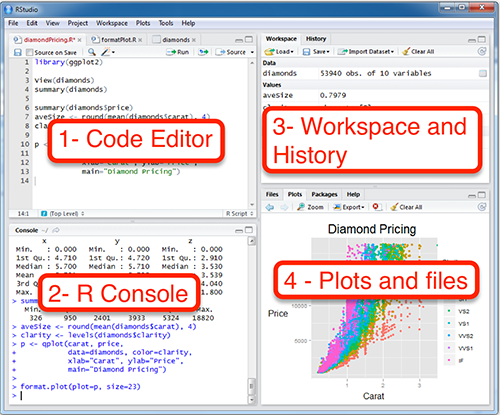
\includegraphics[width=6.94in]{images/01_01_rstudio}

Существуют разные типы пользователей: одни любят работать в консоли (на картинке это \textbf{2 --- R Console}), другие предпочитают скрипты (\textbf{1 --- Code Editor}). Консоль позволяет иметь интерактивный режим команда-ответ, а скрипт является по сути текстовым документом, фрагменты которого можно для отладки запускать в консоли.

\textbf{3 --- Workspace and History}: Здесь можно увидеть переменные. Это поле будет автоматически обновляться по мере того, как Вы будете запускать строчки кода и создавать новые переменные. Еще там есть вкладка с историей последних команд, которые были запущены.

\textbf{4 --- Plots and files}: Здесь есть очень много всего. Во-первых, небольшой файловый менеджер, во-вторых, там будут появляться графики, когда вы будете их рисовать. Там же есть вкладка с вашими пакетами (Packages) и Help по функциям. Но об этом потом.

\hypertarget{r}{%
\section{Введение в R}\label{r}}

\hypertarget{calc}{%
\subsection{R как калькулятор}\label{calc}}

Ой-ей, консоль, скрипт че-то все непонятно.\\
Давайте начнем с самого простого и попробуем использовать R как простой калькулятор. \texttt{+}, \texttt{-}, \texttt{*}, \texttt{/}, \texttt{\^{}} (степень), \texttt{()} и т.д.

Просто запускайте в консоли пока не надоест:

\begin{Shaded}
\begin{Highlighting}[]
\DecValTok{40}\OperatorTok{+}\DecValTok{2}
\end{Highlighting}
\end{Shaded}

\begin{verbatim}
## [1] 42
\end{verbatim}

\begin{Shaded}
\begin{Highlighting}[]
\DecValTok{3-2}
\end{Highlighting}
\end{Shaded}

\begin{verbatim}
## [1] 1
\end{verbatim}

\begin{Shaded}
\begin{Highlighting}[]
\DecValTok{5}\OperatorTok{*}\DecValTok{6}
\end{Highlighting}
\end{Shaded}

\begin{verbatim}
## [1] 30
\end{verbatim}

\begin{Shaded}
\begin{Highlighting}[]
\DecValTok{99}\OperatorTok{/}\DecValTok{9}
\end{Highlighting}
\end{Shaded}

\begin{verbatim}
## [1] 11
\end{verbatim}

\begin{Shaded}
\begin{Highlighting}[]
\DecValTok{2}\OperatorTok{^}\DecValTok{3}
\end{Highlighting}
\end{Shaded}

\begin{verbatim}
## [1] 8
\end{verbatim}

\begin{Shaded}
\begin{Highlighting}[]
\NormalTok{(}\DecValTok{2}\OperatorTok{+}\DecValTok{2}\NormalTok{)}\OperatorTok{*}\DecValTok{2}
\end{Highlighting}
\end{Shaded}

\begin{verbatim}
## [1] 8
\end{verbatim}

Ничего сложного, верно? Вводим выражение и получаем результат. Порядок выполнения арифметических операций как в математике, так что не забывайте про скобочки.

\begin{quote}
Если Вы не уверены в том, какие операции имеют приоритет, то используйте скобочки, чтобы точно обозначить, в каком порядке нужно производить операции.
\end{quote}

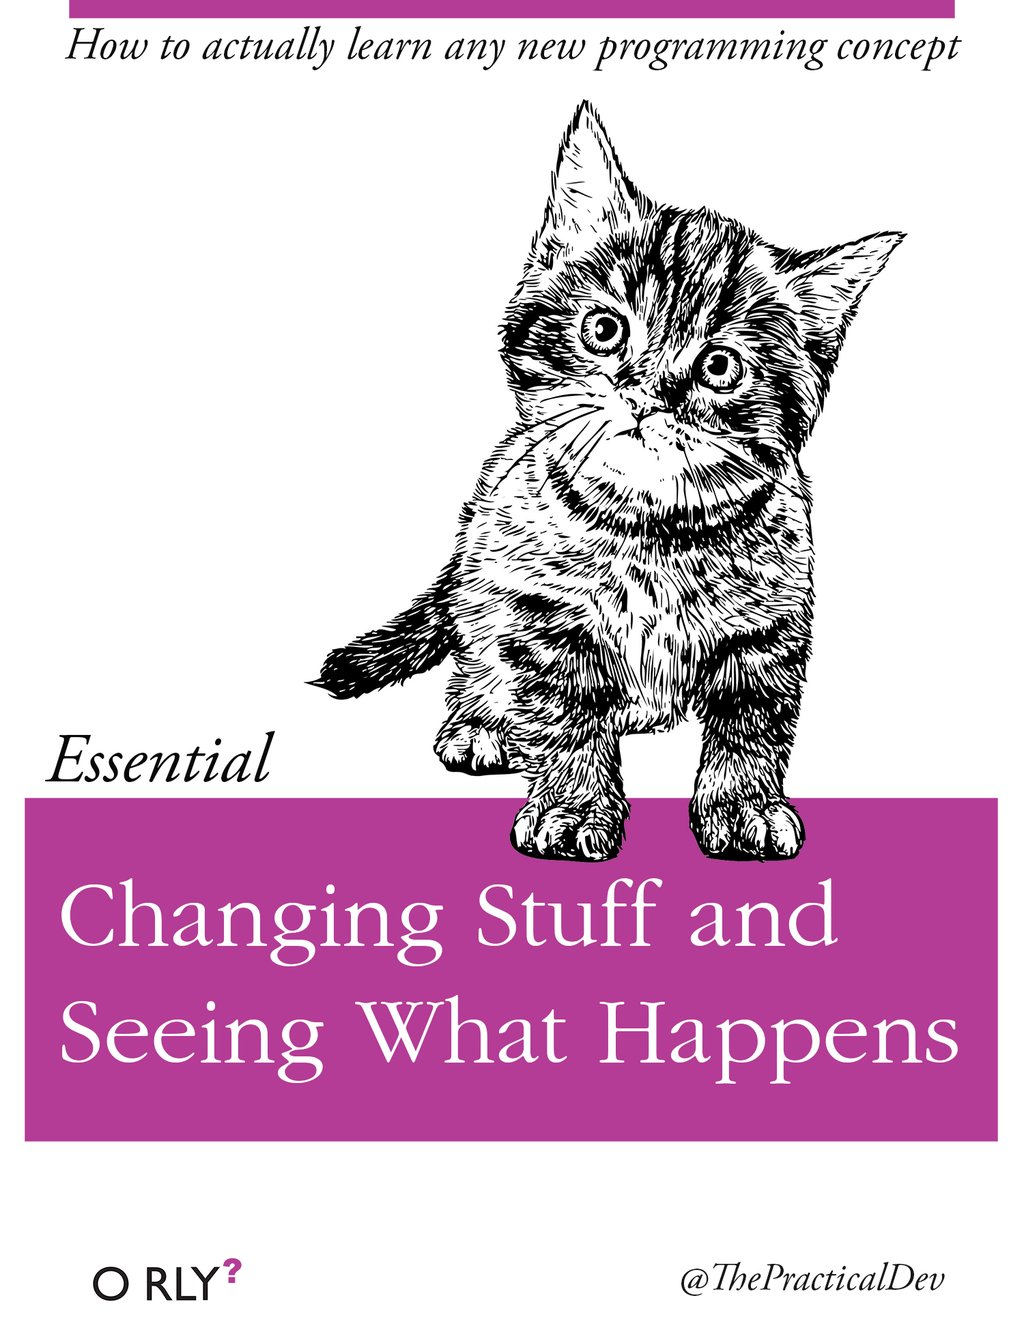
\includegraphics{images/ThePracticalDev_2016-Apr-13.jpg}

\hypertarget{func}{%
\subsection{Функции}\label{func}}

Давайте теперь извлечем корень из какого-нибудь числа. В принципе, тем, кто помнит школьный курс математики, возведения в степень вполне достаточно:

\begin{Shaded}
\begin{Highlighting}[]
\DecValTok{16}\OperatorTok{^}\FloatTok{0.5}
\end{Highlighting}
\end{Shaded}

\begin{verbatim}
## [1] 4
\end{verbatim}

Ну а если нет, то можете воспользоваться специальной \textbf{функцией}: это обычно какие-то буквенные символы с круглыми скобками сразу после названия функции. Мы подаем на вход (внутрь скобочек) какие-то данные, внутри этих функций происходят какие-то вычисления, которые выдает в ответ какие-то другие данные (или же функция записывает файл, рисует график и т.д.).

Вот, например, функция для корня:

\begin{Shaded}
\begin{Highlighting}[]
\KeywordTok{sqrt}\NormalTok{(}\DecValTok{16}\NormalTok{)}
\end{Highlighting}
\end{Shaded}

\begin{verbatim}
## [1] 4
\end{verbatim}

\begin{quote}
R --- case-sensitive язык, т.е. регистр важен. \texttt{SQRT(16)} не будет работать.
\end{quote}

А вот так выглядит функция логарифма:

\begin{Shaded}
\begin{Highlighting}[]
\KeywordTok{log}\NormalTok{(}\DecValTok{8}\NormalTok{)}
\end{Highlighting}
\end{Shaded}

\begin{verbatim}
## [1] 2.079442
\end{verbatim}

Так, вроде бы все нормально, но\ldots{} Если Вы еще что-то помните из школьной математики, то должны понимать, что что-то здесь не так.

Здесь не хватает основания логарифма!

\begin{quote}
Логарифм --- показатель степени, в которую надо возвести число, называемое основанием, чтобы получить данное число.
\end{quote}

То есть у логарифма 8 по основанию 2 будет значение 3:

\(\log_2 8 = 3\)

То есть если возвести 2 в степень 3 у нас будет 8:

\(2^3 = 8\)

Только наша функция считает все как-то не так.

Чтобы понять, что происходит, нам нужно залезть в хэлп этой функции:

\begin{Shaded}
\begin{Highlighting}[]
\NormalTok{?log}
\end{Highlighting}
\end{Shaded}

Справа внизу в RStudio появится вот такое окно:

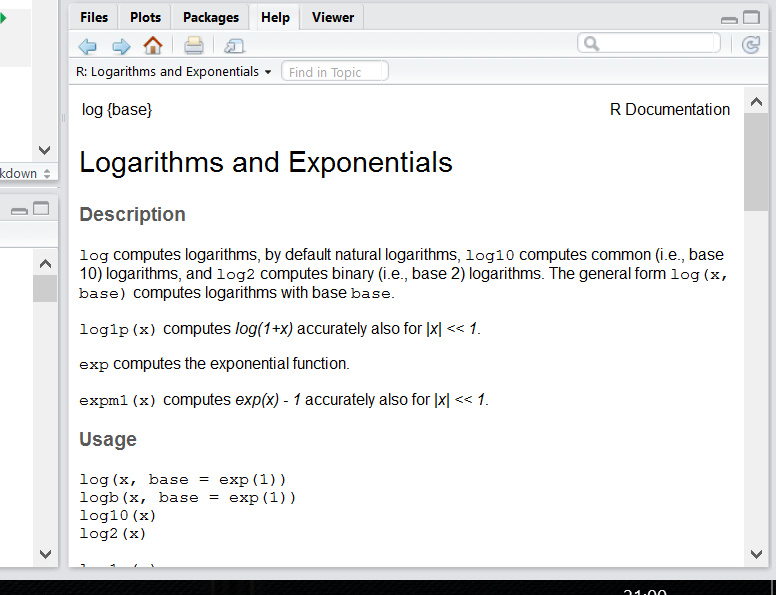
\includegraphics{images/help.png}

Действительно, у этой функции есть еще аргумент \emph{\texttt{base\ =}}. По дефолту он равен числу Эйлера (2.7182818\ldots), т.е. функция считает натуральный логарифм.
В большинстве функций R есть какой-то основной инпут --- данные в том или ином формате, а есть и дополнительные параметры, которые можно прописывать вручную, если параметры по умолчанию нас не устраивают.

\begin{Shaded}
\begin{Highlighting}[]
\KeywordTok{log}\NormalTok{(}\DataTypeTok{x =} \DecValTok{8}\NormalTok{, }\DataTypeTok{base =} \DecValTok{2}\NormalTok{)}
\end{Highlighting}
\end{Shaded}

\begin{verbatim}
## [1] 3
\end{verbatim}

\ldots или просто (если Вы уверены в порядке аргументов):

\begin{Shaded}
\begin{Highlighting}[]
\KeywordTok{log}\NormalTok{(}\DecValTok{8}\NormalTok{,}\DecValTok{2}\NormalTok{)}
\end{Highlighting}
\end{Shaded}

\begin{verbatim}
## [1] 3
\end{verbatim}

Более того, Вы можете использовать оутпут одних функций как инпут для других:

\begin{Shaded}
\begin{Highlighting}[]
\KeywordTok{log}\NormalTok{(}\DecValTok{8}\NormalTok{, }\KeywordTok{sqrt}\NormalTok{(}\DecValTok{4}\NormalTok{))}
\end{Highlighting}
\end{Shaded}

\begin{verbatim}
## [1] 3
\end{verbatim}

Если эксплицитно писать имена аргументов, то их порядок в функции не важен:

\begin{Shaded}
\begin{Highlighting}[]
\KeywordTok{log}\NormalTok{(}\DataTypeTok{base =} \DecValTok{2}\NormalTok{, }\DataTypeTok{x =} \DecValTok{8}\NormalTok{)}
\end{Highlighting}
\end{Shaded}

\begin{verbatim}
## [1] 3
\end{verbatim}

А еще можно недописывать имена аргументов, если они не совпадают с другими:

\begin{Shaded}
\begin{Highlighting}[]
\KeywordTok{log}\NormalTok{(}\DataTypeTok{b =} \DecValTok{2}\NormalTok{, }\DataTypeTok{x =} \DecValTok{8}\NormalTok{)}
\end{Highlighting}
\end{Shaded}

\begin{verbatim}
## [1] 3
\end{verbatim}

Мы еще много раз будем возвращаться к функциям. Вообще, функции --- это одна из важнейших штук в R (примерно так же как и в Python). Мы будем создавать свои функции, использовать функции как инпут для функций и многое-многое другое. В R очень крутые возможности работы с функциями. Поэтому подружитесь с функциями, они клевые.

\begin{quote}
Арифметические знаки, которые мы использовали: +,-,/,\^{} и т.д. называются \textbf{операторами} и на самом деле тоже являются функциями:
\end{quote}

\begin{Shaded}
\begin{Highlighting}[]
\StringTok{'+'}\NormalTok{(}\DecValTok{3}\NormalTok{,}\DecValTok{4}\NormalTok{)}
\end{Highlighting}
\end{Shaded}

\begin{verbatim}
## [1] 7
\end{verbatim}

\hypertarget{variables}{%
\subsection{Переменные}\label{variables}}

Важная штука в программировании на практически любом языке --- возможность сохранять значения в \textbf{переменных}. В R это обычно делается с помощью вот этих символов: \emph{\textless-} (но можно использовать и обычное \emph{=}, хотя это не очень принято). Для этого есть удобное сочетание клавиш: нажмите одновременно \texttt{Alt\ -} (или \texttt{option\ -} на Маке).

\begin{Shaded}
\begin{Highlighting}[]
\NormalTok{a <-}\StringTok{ }\DecValTok{2}
\NormalTok{a}
\end{Highlighting}
\end{Shaded}

\begin{verbatim}
## [1] 2
\end{verbatim}

После присвоения переменная появляется во вкладке \textbf{Environment} в RStudio:

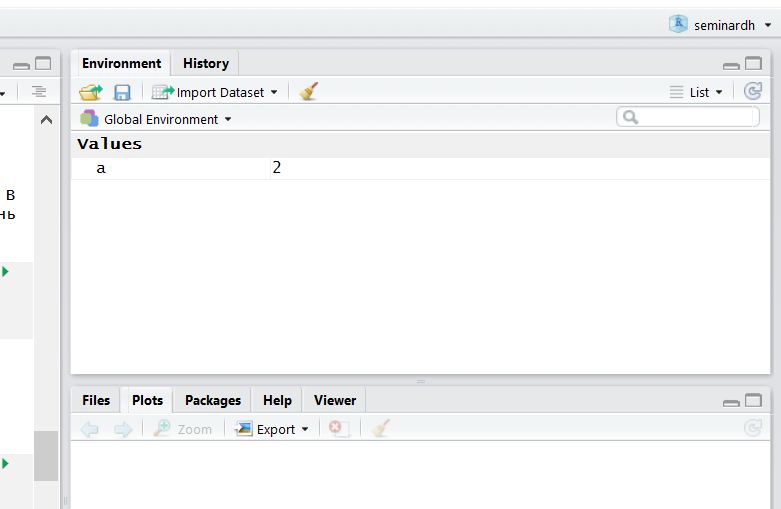
\includegraphics{images/env.png}

Можно использовать переменные в функциях и просто вычислениях:

\begin{Shaded}
\begin{Highlighting}[]
\NormalTok{b <-}\StringTok{ }\NormalTok{a}\OperatorTok{^}\NormalTok{a}\OperatorTok{+}\NormalTok{a}\OperatorTok{*}\NormalTok{a}
\NormalTok{b}
\end{Highlighting}
\end{Shaded}

\begin{verbatim}
## [1] 8
\end{verbatim}

\begin{Shaded}
\begin{Highlighting}[]
\KeywordTok{log}\NormalTok{(b,a)}
\end{Highlighting}
\end{Shaded}

\begin{verbatim}
## [1] 3
\end{verbatim}

Вы можете сравнивать разные переменные:

\begin{Shaded}
\begin{Highlighting}[]
\NormalTok{a }\OperatorTok{==}\StringTok{ }\NormalTok{b}
\end{Highlighting}
\end{Shaded}

\begin{verbatim}
## [1] FALSE
\end{verbatim}

Заметьте, что сравнивая две переменные мы используем два знака равно ==, а не один =. Иначе это будет означать присвоение.

\begin{Shaded}
\begin{Highlighting}[]
\NormalTok{a =}\StringTok{ }\NormalTok{b}
\NormalTok{a}
\end{Highlighting}
\end{Shaded}

\begin{verbatim}
## [1] 8
\end{verbatim}

Теперь Вы сможете понять комикс про восстание роботов на следующей странице (пусть он и совсем про другой язык программирования)

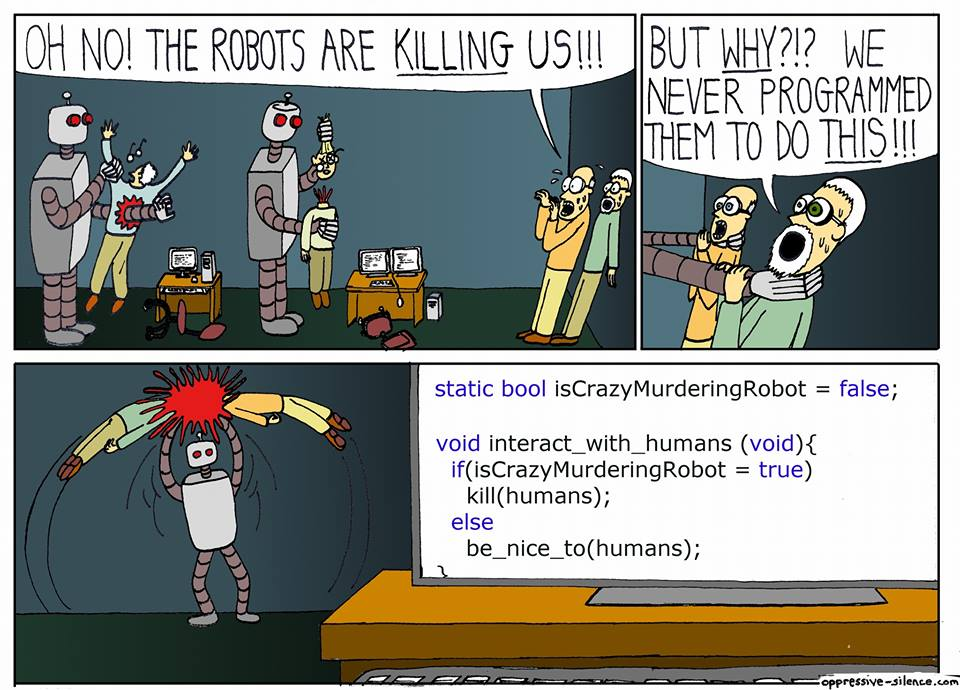
\includegraphics{images/WaCM5x3mvQM.jpg}

Этот комикс объясняет, как важно не путать присваивание и сравнение \emph{(хотя я иногда путаю до сих пор =( )}.

Иногда нам нужно проверить на \emph{не}равенство:

\begin{Shaded}
\begin{Highlighting}[]
\NormalTok{a <-}\StringTok{ }\DecValTok{2}
\NormalTok{b <-}\StringTok{ }\DecValTok{3}

\NormalTok{a}\OperatorTok{==}\NormalTok{b}
\end{Highlighting}
\end{Shaded}

\begin{verbatim}
## [1] FALSE
\end{verbatim}

\begin{Shaded}
\begin{Highlighting}[]
\NormalTok{a}\OperatorTok{!=}\NormalTok{b}
\end{Highlighting}
\end{Shaded}

\begin{verbatim}
## [1] TRUE
\end{verbatim}

Восклицательный язык в программировании вообще и в R в частности стандартно означает отрицание.

Еще мы можем сравнивать на больше/меньше:

\begin{Shaded}
\begin{Highlighting}[]
\NormalTok{a}\OperatorTok{>}\NormalTok{b}
\end{Highlighting}
\end{Shaded}

\begin{verbatim}
## [1] FALSE
\end{verbatim}

\begin{Shaded}
\begin{Highlighting}[]
\NormalTok{a}\OperatorTok{<}\NormalTok{b}
\end{Highlighting}
\end{Shaded}

\begin{verbatim}
## [1] TRUE
\end{verbatim}

\begin{Shaded}
\begin{Highlighting}[]
\NormalTok{a}\OperatorTok{>=}\NormalTok{b}
\end{Highlighting}
\end{Shaded}

\begin{verbatim}
## [1] FALSE
\end{verbatim}

\begin{Shaded}
\begin{Highlighting}[]
\NormalTok{a}\OperatorTok{<=}\NormalTok{b}
\end{Highlighting}
\end{Shaded}

\begin{verbatim}
## [1] TRUE
\end{verbatim}

\hypertarget{data_types}{%
\section{Типы данных}\label{data_types}}

До этого момента мы работали только с числами (numeric):

\begin{Shaded}
\begin{Highlighting}[]
\KeywordTok{class}\NormalTok{(a)}
\end{Highlighting}
\end{Shaded}

\begin{verbatim}
## [1] "numeric"
\end{verbatim}

\begin{quote}
Вообще, в R много типов numeric: integer (целые), double (с десятичной дробью), complex (комплексные числа). Последние пишутся так: \texttt{complexnumber\ \textless{}-\ 2+2i}
Однако в R с этим обычно можно вообще не заморачиваться, R сам будет конвертить между форматами при необходимости. Немного подробностей здесь:
\end{quote}

\href{https://stackoverflow.com/questions/23660094/whats-the-difference-between-integer-class-and-numeric-class-in-r}{Разница между numeric и integer}, \href{http://www.r-tutor.com/r-introduction/basic-data-types/complex}{Как работать с комплексными числами в R}

Теперь же нам нужно ознакомиться с двумя другими важными типами данных в R:

\begin{enumerate}
\def\labelenumi{\arabic{enumi}.}
\tightlist
\item
  \textbf{character}: строки символов. Они должны выделяться кавычками. Можно использовать как \texttt{"}, так и \texttt{\textquotesingle{}} (что удобно, когда строчка внутри уже содержит какие-то кавычки).
\end{enumerate}

\begin{Shaded}
\begin{Highlighting}[]
\NormalTok{s <-}\StringTok{ "Всем привет!"}
\NormalTok{s}
\end{Highlighting}
\end{Shaded}

\begin{verbatim}
## [1] "Всем привет!"
\end{verbatim}

\begin{Shaded}
\begin{Highlighting}[]
\KeywordTok{class}\NormalTok{(s)}
\end{Highlighting}
\end{Shaded}

\begin{verbatim}
## [1] "character"
\end{verbatim}

\begin{enumerate}
\def\labelenumi{\arabic{enumi}.}
\setcounter{enumi}{1}
\tightlist
\item
  \textbf{logical}: просто \texttt{TRUE} или \texttt{FALSE}.
\end{enumerate}

\begin{Shaded}
\begin{Highlighting}[]
\NormalTok{t1 <-}\StringTok{ }\OtherTok{TRUE}
\NormalTok{f1 <-}\StringTok{ }\OtherTok{FALSE}

\NormalTok{t1}
\end{Highlighting}
\end{Shaded}

\begin{verbatim}
## [1] TRUE
\end{verbatim}

\begin{Shaded}
\begin{Highlighting}[]
\NormalTok{f1}
\end{Highlighting}
\end{Shaded}

\begin{verbatim}
## [1] FALSE
\end{verbatim}

Вообще, можно еще писать \texttt{T} и \texttt{F} (но не \texttt{True} и \texttt{False}!)

\begin{Shaded}
\begin{Highlighting}[]
\NormalTok{t2 <-}\StringTok{ }\NormalTok{T}
\NormalTok{f2 <-}\StringTok{ }\NormalTok{F}
\end{Highlighting}
\end{Shaded}

Это дурная практика, так как R защищает от перезаписи переменные \texttt{TRUE} и \texttt{FALSE}, но не защищает от этого \texttt{T} и \texttt{F}

\begin{Shaded}
\begin{Highlighting}[]
\OtherTok{TRUE}\NormalTok{ <-}\StringTok{ }\OtherTok{FALSE}
\end{Highlighting}
\end{Shaded}

\begin{verbatim}
## Error in TRUE <- FALSE: invalid (do_set) left-hand side to assignment
\end{verbatim}

\begin{Shaded}
\begin{Highlighting}[]
\OtherTok{TRUE}
\end{Highlighting}
\end{Shaded}

\begin{verbatim}
## [1] TRUE
\end{verbatim}

\begin{Shaded}
\begin{Highlighting}[]
\NormalTok{T <-}\StringTok{ }\OtherTok{FALSE}
\NormalTok{T}
\end{Highlighting}
\end{Shaded}

\begin{verbatim}
## [1] FALSE
\end{verbatim}

Теперь вы можете догадаться, что результаты сравнения, например, числовых или строковых переменных вы можете сохранять в переменные тоже!

\begin{Shaded}
\begin{Highlighting}[]
\NormalTok{comparison <-}\StringTok{ }\NormalTok{a }\OperatorTok{==}\StringTok{ }\NormalTok{b}
\NormalTok{comparison}
\end{Highlighting}
\end{Shaded}

\begin{verbatim}
## [1] FALSE
\end{verbatim}

Это нам очень понадобится, когда мы будем работать с реальными данными: нам нужно будет постоянно вытаскивать какие-то данные из датасета, а это как раз и построено на игре со сравнением переменных.

Чтобы этим хорошо уметь пользоваться, нам нужно еще освоить как работать с логическими операторами. Про один мы немного уже говорили --- это не (\texttt{!}):

\begin{Shaded}
\begin{Highlighting}[]
\NormalTok{t1}
\end{Highlighting}
\end{Shaded}

\begin{verbatim}
## [1] TRUE
\end{verbatim}

\begin{Shaded}
\begin{Highlighting}[]
\OperatorTok{!}\NormalTok{t1}
\end{Highlighting}
\end{Shaded}

\begin{verbatim}
## [1] FALSE
\end{verbatim}

\begin{Shaded}
\begin{Highlighting}[]
\OperatorTok{!!}\NormalTok{t1 }\CommentTok{#Двойное отрицание!}
\end{Highlighting}
\end{Shaded}

\begin{verbatim}
## [1] TRUE
\end{verbatim}

Еще есть И (выдаст \texttt{TRUE} только в том случае если обе переменные \texttt{TRUE}):

\begin{Shaded}
\begin{Highlighting}[]
\NormalTok{t1}\OperatorTok{&}\NormalTok{t2}
\end{Highlighting}
\end{Shaded}

\begin{verbatim}
## [1] TRUE
\end{verbatim}

\begin{Shaded}
\begin{Highlighting}[]
\NormalTok{t1}\OperatorTok{&}\NormalTok{f1}
\end{Highlighting}
\end{Shaded}

\begin{verbatim}
## [1] FALSE
\end{verbatim}

А еще ИЛИ (выдаст \texttt{TRUE} в случае если хотя бы одна из переменных \texttt{TRUE}):

\begin{Shaded}
\begin{Highlighting}[]
\NormalTok{t1 }\OperatorTok{|}\StringTok{ }\NormalTok{f1}
\end{Highlighting}
\end{Shaded}

\begin{verbatim}
## [1] TRUE
\end{verbatim}

\begin{Shaded}
\begin{Highlighting}[]
\NormalTok{f1 }\OperatorTok{|}\StringTok{ }\NormalTok{f2}
\end{Highlighting}
\end{Shaded}

\begin{verbatim}
## [1] FALSE
\end{verbatim}

Если кому-то вдруг понадобиться другое ИЛИ --- есть функция \texttt{xor()}, принимающий два аргумента.

Поздравляю, мы только что разобрались с самой занудной частью.
Пора переходить к важному и интересному. ВЕКТОРАМ!

\hypertarget{atomic}{%
\section{Вектор}\label{atomic}}

Если у вас не было линейной алгебры (или у вас с ней было все плохо), то просто запомните, что \textbf{вектор} (или \textbf{atomic vector} или \textbf{atomic}) --- это набор (столбик) чисел в определенном порядке.

\begin{quote}
P.S. Если вы привыкли из школьного курса физики считать вектора стрелочками, то не спешите возмущаться и паниковать. Представьте стрелочки как точки из нуля координат \{0,0\} до какой-то точки на координатной плоскости, например, \{2,1\}. Вот последние два числа и будем считать вектором. Поэтому постарайтесь на время выбросить стрелочки из головы.
\end{quote}

На самом деле, мы уже работали с векторами в R, но, возможно, Вы об этом даже не догадывались. Дело в том, что в R нет как таковых ``значений'', \textbf{есть вектора длиной 1}. Такие дела!

Чтобы создать вектор из нескольких значений, нужно воспользоваться функцией \emph{\texttt{c()}}:

\begin{Shaded}
\begin{Highlighting}[]
\KeywordTok{c}\NormalTok{(}\DecValTok{4}\NormalTok{,}\DecValTok{8}\NormalTok{,}\DecValTok{15}\NormalTok{,}\DecValTok{16}\NormalTok{,}\DecValTok{23}\NormalTok{,}\DecValTok{42}\NormalTok{)}
\end{Highlighting}
\end{Shaded}

\begin{verbatim}
## [1]  4  8 15 16 23 42
\end{verbatim}

\begin{Shaded}
\begin{Highlighting}[]
\KeywordTok{c}\NormalTok{(}\StringTok{"Хэй"}\NormalTok{, }\StringTok{"Хэй"}\NormalTok{, }\StringTok{"Ха"}\NormalTok{)}
\end{Highlighting}
\end{Shaded}

\begin{verbatim}
## [1] "Хэй" "Хэй" "Ха"
\end{verbatim}

\begin{quote}
Одна из самых мерзких и раздражающих причин ошибок в коде --- это использование \texttt{с} из кириллицы вместо \texttt{c} из латиницы. Видите разницу? И я не вижу. А R видит. И об этом сообщает:
\end{quote}

\begin{Shaded}
\begin{Highlighting}[]
\NormalTok{с(}\DecValTok{3}\NormalTok{, }\DecValTok{4}\NormalTok{, }\DecValTok{5}\NormalTok{)}
\end{Highlighting}
\end{Shaded}

\begin{verbatim}
## Error in с(3, 4, 5): could not find function "с"
\end{verbatim}

Для создания числовых векторов есть удобный \textbf{оператор} \texttt{:}

\begin{Shaded}
\begin{Highlighting}[]
\DecValTok{1}\OperatorTok{:}\DecValTok{10}
\end{Highlighting}
\end{Shaded}

\begin{verbatim}
##  [1]  1  2  3  4  5  6  7  8  9 10
\end{verbatim}

\begin{Shaded}
\begin{Highlighting}[]
\DecValTok{5}\OperatorTok{:-}\DecValTok{3}
\end{Highlighting}
\end{Shaded}

\begin{verbatim}
## [1]  5  4  3  2  1  0 -1 -2 -3
\end{verbatim}

Этот оператор создает вектор от первого числа до второго с шагом 1. Вы не представляете, как часто эта штука нам пригодится\ldots{} Если же нужно сделать вектор с другим шагом, то есть функция \texttt{seq()}:

\begin{Shaded}
\begin{Highlighting}[]
\KeywordTok{seq}\NormalTok{(}\DecValTok{10}\NormalTok{,}\DecValTok{100}\NormalTok{, }\DataTypeTok{by =} \DecValTok{10}\NormalTok{)}
\end{Highlighting}
\end{Shaded}

\begin{verbatim}
##  [1]  10  20  30  40  50  60  70  80  90 100
\end{verbatim}

Кроме того, можно задавать не шаг, а длину вектора. Тогда шаг функция \texttt{seq()} посчитает сама:

\begin{Shaded}
\begin{Highlighting}[]
\KeywordTok{seq}\NormalTok{(}\DecValTok{1}\NormalTok{,}\DecValTok{13}\NormalTok{, }\DataTypeTok{length.out =} \DecValTok{4}\NormalTok{)}
\end{Highlighting}
\end{Shaded}

\begin{verbatim}
## [1]  1  5  9 13
\end{verbatim}

Другая функция --- \texttt{rep()} --- позволяет создавать вектора с повторяющимися значениями. Первый аргумент --- значение, которое нужно повторять, а второй аргумент --- сколько раз повторять.

\begin{Shaded}
\begin{Highlighting}[]
\KeywordTok{rep}\NormalTok{(}\DecValTok{1}\NormalTok{, }\DecValTok{5}\NormalTok{)}
\end{Highlighting}
\end{Shaded}

\begin{verbatim}
## [1] 1 1 1 1 1
\end{verbatim}

И первый, и второй аргумент могут быть векторами!

\begin{Shaded}
\begin{Highlighting}[]
\KeywordTok{rep}\NormalTok{(}\DecValTok{1}\OperatorTok{:}\DecValTok{3}\NormalTok{, }\DecValTok{3}\NormalTok{)}
\end{Highlighting}
\end{Shaded}

\begin{verbatim}
## [1] 1 2 3 1 2 3 1 2 3
\end{verbatim}

\begin{Shaded}
\begin{Highlighting}[]
\KeywordTok{rep}\NormalTok{(}\DecValTok{1}\OperatorTok{:}\DecValTok{3}\NormalTok{, }\DecValTok{1}\OperatorTok{:}\DecValTok{3}\NormalTok{)}
\end{Highlighting}
\end{Shaded}

\begin{verbatim}
## [1] 1 2 2 3 3 3
\end{verbatim}

Еще можно объединять вектора (что мы, по сути, и делали, просто с векторами длиной 1):

\begin{Shaded}
\begin{Highlighting}[]
\NormalTok{v1 <-}\StringTok{ }\KeywordTok{c}\NormalTok{(}\StringTok{"Hey"}\NormalTok{, }\StringTok{"Ho"}\NormalTok{)}
\NormalTok{v2 <-}\StringTok{ }\KeywordTok{c}\NormalTok{(}\StringTok{"Let's"}\NormalTok{, }\StringTok{"Go!"}\NormalTok{)}
\KeywordTok{c}\NormalTok{(v1,v2)}
\end{Highlighting}
\end{Shaded}

\begin{verbatim}
## [1] "Hey"   "Ho"    "Let's" "Go!"
\end{verbatim}

\hypertarget{coercion}{%
\subsection{Coercion}\label{coercion}}

Что будет, если вы объедините два вектора с значениями разных типов? Ошибка?
Мы уже обсуждали, что в \emph{atomic} может быть только один тип данных. В некоторых языках программирования при операции с данными разных типов мы бы получили ошибку. А вот в R при несовпадении типов пройзойдет попытка привести типы к ``общему знаменателю'', то есть конвертировать данные в более ``широкий'' тип.

Например:

\begin{Shaded}
\begin{Highlighting}[]
\KeywordTok{c}\NormalTok{(}\OtherTok{FALSE}\NormalTok{, }\DecValTok{2}\NormalTok{)}
\end{Highlighting}
\end{Shaded}

\begin{verbatim}
## [1] 0 2
\end{verbatim}

\texttt{FALSE} превратился в \texttt{0} (а \texttt{TRUE} превратился бы в \texttt{1}), чтобы можно было оба значения объединить в вектор. То же самое произошло бы в случае операций с векторами:

\begin{Shaded}
\begin{Highlighting}[]
\DecValTok{2} \OperatorTok{+}\StringTok{ }\OtherTok{TRUE}
\end{Highlighting}
\end{Shaded}

\begin{verbatim}
## [1] 3
\end{verbatim}

Это называется \textbf{coercion}.
Более сложный пример:

\begin{Shaded}
\begin{Highlighting}[]
\KeywordTok{c}\NormalTok{(}\OtherTok{TRUE}\NormalTok{, }\DecValTok{3}\NormalTok{, }\StringTok{"Привет"}\NormalTok{)}
\end{Highlighting}
\end{Shaded}

\begin{verbatim}
## [1] "TRUE"   "3"      "Привет"
\end{verbatim}

У R есть иерархия коэрсинга:
\texttt{NULL\ \textless{}\ raw\ \textless{}\ logical\ \textless{}\ integer\ \textless{}\ double\ \textless{}\ complex\ \textless{}\ character\ \textless{}\ list\ \textless{}\ expression}.
Мы из этого списка еще многого не знаем, сейчас важно запомнить, что логические данные --- \texttt{TRUE} и \texttt{FALSE} --- превращаются в \texttt{0} и \texttt{1} соответственно, а \texttt{0} и \texttt{1} в строчки \texttt{"0"} и \texttt{"1"}.

Если Вы боитесь полагаться на coercion, то можете воспользоваться функциями \texttt{as.нужныйтипданных}:

\begin{Shaded}
\begin{Highlighting}[]
\KeywordTok{as.numeric}\NormalTok{(}\KeywordTok{c}\NormalTok{(}\OtherTok{TRUE}\NormalTok{, }\OtherTok{FALSE}\NormalTok{, }\OtherTok{FALSE}\NormalTok{))}
\end{Highlighting}
\end{Shaded}

\begin{verbatim}
## [1] 1 0 0
\end{verbatim}

\begin{Shaded}
\begin{Highlighting}[]
\KeywordTok{as.character}\NormalTok{(}\KeywordTok{as.numeric}\NormalTok{(}\KeywordTok{c}\NormalTok{(}\OtherTok{TRUE}\NormalTok{, }\OtherTok{FALSE}\NormalTok{, }\OtherTok{FALSE}\NormalTok{)))}
\end{Highlighting}
\end{Shaded}

\begin{verbatim}
## [1] "1" "0" "0"
\end{verbatim}

Можно превращать и обратно, например, строковые значения в числовые. Если среди числа встретится буква или другой неподходящий знак, то мы получим предупреждение \texttt{NA} --- пропущенное значение (мы очень скоро научимся с ними работать).

\begin{Shaded}
\begin{Highlighting}[]
\KeywordTok{as.numeric}\NormalTok{(}\KeywordTok{c}\NormalTok{(}\StringTok{"1"}\NormalTok{, }\StringTok{"2"}\NormalTok{, }\StringTok{"три"}\NormalTok{))}
\end{Highlighting}
\end{Shaded}

\begin{verbatim}
## Warning: NAs introduced by coercion
\end{verbatim}

\begin{verbatim}
## [1]  1  2 NA
\end{verbatim}

\hypertarget{vector_op}{%
\subsection{Операции с векторами}\label{vector_op}}

Все те арифметические операции, что мы использовали ранее, можно использовать с векторами одинаковой длины:

\begin{Shaded}
\begin{Highlighting}[]
\NormalTok{n <-}\StringTok{ }\DecValTok{1}\OperatorTok{:}\DecValTok{4}
\NormalTok{m <-}\StringTok{ }\DecValTok{4}\OperatorTok{:}\DecValTok{1}
\NormalTok{n }\OperatorTok{+}\StringTok{ }\NormalTok{m}
\end{Highlighting}
\end{Shaded}

\begin{verbatim}
## [1] 5 5 5 5
\end{verbatim}

\begin{Shaded}
\begin{Highlighting}[]
\NormalTok{n }\OperatorTok{-}\StringTok{ }\NormalTok{m}
\end{Highlighting}
\end{Shaded}

\begin{verbatim}
## [1] -3 -1  1  3
\end{verbatim}

\begin{Shaded}
\begin{Highlighting}[]
\NormalTok{n }\OperatorTok{*}\StringTok{ }\NormalTok{m}
\end{Highlighting}
\end{Shaded}

\begin{verbatim}
## [1] 4 6 6 4
\end{verbatim}

\begin{Shaded}
\begin{Highlighting}[]
\NormalTok{n }\OperatorTok{/}\StringTok{ }\NormalTok{m}
\end{Highlighting}
\end{Shaded}

\begin{verbatim}
## [1] 0.2500000 0.6666667 1.5000000 4.0000000
\end{verbatim}

\begin{Shaded}
\begin{Highlighting}[]
\NormalTok{n }\OperatorTok{^}\StringTok{ }\NormalTok{m }\OperatorTok{+}\StringTok{ }\NormalTok{m }\OperatorTok{*}\StringTok{ }\NormalTok{(n }\OperatorTok{-}\StringTok{ }\NormalTok{m)}
\end{Highlighting}
\end{Shaded}

\begin{verbatim}
## [1] -11   5  11   7
\end{verbatim}

\begin{quote}
Если после какого-нибудь MATLAB Вы привыкли, что по умолчанию операторы работают по правилам линейной алгебры и \texttt{m*n} будет давать скалярное произведение (dot product), то снова нет. Для скалярного произведения нужно использовать операторы с \texttt{\%} по краям:
\end{quote}

\begin{Shaded}
\begin{Highlighting}[]
\NormalTok{n }\OperatorTok\StringTok{ }\NormalTok{m}
\end{Highlighting}
\end{Shaded}

\begin{verbatim}
##      [,1]
## [1,]   20
\end{verbatim}

\begin{quote}
Абсолютно так же и с операциями с матрицами в R, хотя про матрицы будет немного позже.
\end{quote}

В принципе, большинство функций в R, которые работают с отдельными значениями, так же хорошо работают и с целыми векторами. Скажем, Вы хотите извлечь корень из нескольких чисел, для этого не нужны никакие циклы (как это обычно делается в других языках программирования). Можно просто ``скормить'' вектор функции и получить результат применения функции к каждому элементу вектора:

\begin{Shaded}
\begin{Highlighting}[]
\KeywordTok{sqrt}\NormalTok{(}\DecValTok{1}\OperatorTok{:}\DecValTok{10}\NormalTok{)}
\end{Highlighting}
\end{Shaded}

\begin{verbatim}
##  [1] 1.000000 1.414214 1.732051 2.000000 2.236068 2.449490 2.645751
##  [8] 2.828427 3.000000 3.162278
\end{verbatim}

\hypertarget{recycling}{%
\subsection{Recycling}\label{recycling}}

Допустим мы хотим совершить какую-нибудь операцию с двумя векторами. Как мы убедились, с этим обычно нет никаких проблем, если они совпадают по длине. А что если вектора не совпадают по длине?
Ничего страшного! Здесь будет работать правило ресайклинга (\textbf{recycling} = \emph{правило переписывания}). Это означает, что если короткий вектор кратен по длине длинному, то он будет повторять короткий необходимое количество раз:

\begin{Shaded}
\begin{Highlighting}[]
\NormalTok{n <-}\StringTok{ }\DecValTok{1}\OperatorTok{:}\DecValTok{4}
\NormalTok{m <-}\StringTok{ }\DecValTok{1}\OperatorTok{:}\DecValTok{2}
\NormalTok{n }\OperatorTok{*}\StringTok{ }\NormalTok{m}
\end{Highlighting}
\end{Shaded}

\begin{verbatim}
## [1] 1 4 3 8
\end{verbatim}

А что будет, если совершать операции с вектором и отдельным значением? Можно считать это частным случаем ресайклинга: короткий вектор длиной 1 будет повторятся столько раз, сколько нужно, чтобы он совпадал по длине с длинным:

\begin{Shaded}
\begin{Highlighting}[]
\NormalTok{n }\OperatorTok{*}\StringTok{ }\DecValTok{2}
\end{Highlighting}
\end{Shaded}

\begin{verbatim}
## [1] 2 4 6 8
\end{verbatim}

Если же меньший вектор не кратен большему (например, один из них длиной 3, а другой длиной 4), то R посчитает результат, но выдаст предупреждение.

\begin{Shaded}
\begin{Highlighting}[]
\NormalTok{n }\OperatorTok{+}\StringTok{ }\KeywordTok{c}\NormalTok{(}\DecValTok{3}\NormalTok{,}\DecValTok{4}\NormalTok{,}\DecValTok{5}\NormalTok{)}
\end{Highlighting}
\end{Shaded}

\begin{verbatim}
## Warning in n + c(3, 4, 5): longer object length is not a multiple of
## shorter object length
\end{verbatim}

\begin{verbatim}
## [1] 4 6 8 7
\end{verbatim}

Проблема в том, что эти предупреждения могут в неожиданный момент стать причиной ошибок. Поэтому не стоит полагаться на ресайклинг некратных по длине векторов. \href{https://stackoverflow.com/questions/6555651/under-what-circumstances-does-r-recycle}{См. здесь}. А вот ресайклинг кратных по длине векторов --- это очень удобная штука, которая используется очень часто.

\hypertarget{index_atomic}{%
\subsection{Индексирование векторов}\label{index_atomic}}

Итак, мы подошли к одному из самых сложных моментов. И одному из основных. От того, как хорошо вы научись с этим работать, зависит весь Ваш дальнейший успех на R-поприще!

Речь пойдет об \textbf{индексировании} векторов. Задача, которую Вам придется решать каждые пять минут работы в R - как выбрать из вектора (или же списка, матрицы и датафрейма) какую-то его часть. Для этого используются квадратные скобочки \texttt{{[}{]}} (не круглые - они для функций!).

Самое простое - индексировать по номеру индекса, т.е. порядку значения в векторе.

\begin{Shaded}
\begin{Highlighting}[]
\NormalTok{n <-}\StringTok{ }\DecValTok{1}\OperatorTok{:}\DecValTok{10}
\NormalTok{n[}\DecValTok{1}\NormalTok{]}
\end{Highlighting}
\end{Shaded}

\begin{verbatim}
## [1] 1
\end{verbatim}

\begin{Shaded}
\begin{Highlighting}[]
\NormalTok{n[}\DecValTok{10}\NormalTok{]}
\end{Highlighting}
\end{Shaded}

\begin{verbatim}
## [1] 10
\end{verbatim}

\begin{quote}
Если вы знакомы с другими языками программирования (не MATLAB, там все так же) и уже научились думать, что индексация с 0 --- это очень удобно и очень правильно (ну или просто свыклись с этим), то в R Вам придется переучиться обратно. Здесь первый индекс --- это 1, а последний равен длине вектора --- ее можно узнать с помощью функции \texttt{length()}. С обоих сторон индексы берутся включительно.
\end{quote}

С помощью индексирования можно не только вытаскивать имеющиеся значения в векторе, но и присваивать им новые:

\begin{Shaded}
\begin{Highlighting}[]
\NormalTok{n[}\DecValTok{3}\NormalTok{] <-}\StringTok{ }\DecValTok{20}
\NormalTok{n}
\end{Highlighting}
\end{Shaded}

\begin{verbatim}
##  [1]  1  2 20  4  5  6  7  8  9 10
\end{verbatim}

Конечно, можно использовать целые векторы для индексирования:

\begin{Shaded}
\begin{Highlighting}[]
\NormalTok{n[}\DecValTok{4}\OperatorTok{:}\DecValTok{7}\NormalTok{]}
\end{Highlighting}
\end{Shaded}

\begin{verbatim}
## [1] 4 5 6 7
\end{verbatim}

\begin{Shaded}
\begin{Highlighting}[]
\NormalTok{n[}\DecValTok{10}\OperatorTok{:}\DecValTok{1}\NormalTok{]}
\end{Highlighting}
\end{Shaded}

\begin{verbatim}
##  [1] 10  9  8  7  6  5  4 20  2  1
\end{verbatim}

Индексирование с минусом выдаст вам все значения вектора кроме выбранных (простите, пользователя Python, которые ожидают здесь отсчет с конца\ldots):

\begin{Shaded}
\begin{Highlighting}[]
\NormalTok{n[}\OperatorTok{-}\DecValTok{1}\NormalTok{]}
\end{Highlighting}
\end{Shaded}

\begin{verbatim}
## [1]  2 20  4  5  6  7  8  9 10
\end{verbatim}

\begin{Shaded}
\begin{Highlighting}[]
\NormalTok{n[}\KeywordTok{c}\NormalTok{(}\OperatorTok{-}\DecValTok{4}\NormalTok{, }\DecValTok{-5}\NormalTok{)]}
\end{Highlighting}
\end{Shaded}

\begin{verbatim}
## [1]  1  2 20  6  7  8  9 10
\end{verbatim}

Более того, можно использовать логический вектор для индексирования. В этом случае нужен логический вектор такой же длины:

\begin{Shaded}
\begin{Highlighting}[]
\NormalTok{n[}\KeywordTok{c}\NormalTok{(}\OtherTok{TRUE}\NormalTok{,}\OtherTok{FALSE}\NormalTok{,}\OtherTok{TRUE}\NormalTok{,}\OtherTok{FALSE}\NormalTok{,}\OtherTok{TRUE}\NormalTok{,}\OtherTok{FALSE}\NormalTok{,}\OtherTok{TRUE}\NormalTok{,}\OtherTok{FALSE}\NormalTok{,}\OtherTok{TRUE}\NormalTok{,}\OtherTok{FALSE}\NormalTok{)]}
\end{Highlighting}
\end{Shaded}

\begin{verbatim}
## [1]  1 20  5  7  9
\end{verbatim}

Ну а если они не равны, то тут будет снова работать правило ресайклинга!

\begin{Shaded}
\begin{Highlighting}[]
\NormalTok{n[}\KeywordTok{c}\NormalTok{(}\OtherTok{TRUE}\NormalTok{,}\OtherTok{FALSE}\NormalTok{)] }\CommentTok{#то же самое - recycling rule!}
\end{Highlighting}
\end{Shaded}

\begin{verbatim}
## [1]  1 20  5  7  9
\end{verbatim}

Есть еще один способ индексирования векторов, но он несколько более редкий: индексирование по имени. Дело в том, что для значений векторов можно (но не обязательно) присваивать имена:

\begin{Shaded}
\begin{Highlighting}[]
\NormalTok{my_named_vector <-}\StringTok{ }\KeywordTok{c}\NormalTok{(}\DataTypeTok{first =} \DecValTok{1}\NormalTok{, }\DataTypeTok{second =} \DecValTok{2}\NormalTok{, }\DataTypeTok{third =} \DecValTok{3}\NormalTok{)}
\NormalTok{my_named_vector[}\StringTok{'first'}\NormalTok{]}
\end{Highlighting}
\end{Shaded}

\begin{verbatim}
## first 
##     1
\end{verbatim}

А еще можно ``вытаскивать'' имена из вектора с помощью функции \texttt{names()} и присваивать таким образом новые.

\begin{Shaded}
\begin{Highlighting}[]
\NormalTok{d <-}\StringTok{ }\DecValTok{1}\OperatorTok{:}\DecValTok{4}
\KeywordTok{names}\NormalTok{(d) <-}\StringTok{ }\NormalTok{letters[}\DecValTok{1}\OperatorTok{:}\DecValTok{4}\NormalTok{]}
\NormalTok{d[}\StringTok{"a"}\NormalTok{]}
\end{Highlighting}
\end{Shaded}

\begin{verbatim}
## a 
## 1
\end{verbatim}

\begin{quote}
\texttt{letters} - это ``зашитая'' в R константа - вектор букв от a до z. Иногда это очень удобно! Кроме того, есть константа \texttt{LETTERS} - то же самое, но заглавными буквами. А еще есть названия месяцев на английском и числовая константа \texttt{pi}.
\end{quote}

Теперь посчитаем среднее вектора \texttt{n}:

\begin{Shaded}
\begin{Highlighting}[]
\KeywordTok{mean}\NormalTok{(n)}
\end{Highlighting}
\end{Shaded}

\begin{verbatim}
## [1] 7.2
\end{verbatim}

А как вытащить все значения, которые больше среднего?

Сначала получим логический вектор --- какие значения больше среднего:

\begin{Shaded}
\begin{Highlighting}[]
\NormalTok{larger <-}\StringTok{ }\NormalTok{n }\OperatorTok{>}\StringTok{ }\KeywordTok{mean}\NormalTok{(n)}
\NormalTok{larger}
\end{Highlighting}
\end{Shaded}

\begin{verbatim}
##  [1] FALSE FALSE  TRUE FALSE FALSE FALSE FALSE  TRUE  TRUE  TRUE
\end{verbatim}

А теперь используем его для индексирования вектора \texttt{n}:

\begin{Shaded}
\begin{Highlighting}[]
\NormalTok{n[larger]}
\end{Highlighting}
\end{Shaded}

\begin{verbatim}
## [1] 20  8  9 10
\end{verbatim}

Можно все это сделать в одну строчку:

\begin{Shaded}
\begin{Highlighting}[]
\NormalTok{n[n}\OperatorTok{>}\KeywordTok{mean}\NormalTok{(n)]}
\end{Highlighting}
\end{Shaded}

\begin{verbatim}
## [1] 20  8  9 10
\end{verbatim}

Предыдущая строчка отражает то, что мы будем постоянно делать в R: вычленять (subset) из данных отдельные куски на основании разных условий.

\hypertarget{na}{%
\subsection{NA --- пропущенные значения}\label{na}}

В реальных данных у нас часто чего-то не хватает. Например, из-за технической ошибки или невнимательности не получилось записать какое-то измерение. Для этого в R есть \texttt{NA}. \texttt{NA} --- это не строка \texttt{"NA"}, не \texttt{0}, не пустая строка \texttt{""} и не \texttt{FALSE}. \texttt{NA} --- это \texttt{NA}.
Большинство операций с векторами, содержащими \texttt{NA} будут выдавать \texttt{NA}:

\begin{Shaded}
\begin{Highlighting}[]
\NormalTok{missed <-}\StringTok{ }\OtherTok{NA}
\NormalTok{missed }\OperatorTok{==}\StringTok{ "NA"}
\end{Highlighting}
\end{Shaded}

\begin{verbatim}
## [1] NA
\end{verbatim}

\begin{Shaded}
\begin{Highlighting}[]
\NormalTok{missed }\OperatorTok{==}\StringTok{ ""}
\end{Highlighting}
\end{Shaded}

\begin{verbatim}
## [1] NA
\end{verbatim}

\begin{Shaded}
\begin{Highlighting}[]
\NormalTok{missed }\OperatorTok{==}\StringTok{ }\OtherTok{NA}
\end{Highlighting}
\end{Shaded}

\begin{verbatim}
## [1] NA
\end{verbatim}

Заметьте: даже сравнение \texttt{NA} c \texttt{NA} выдает \texttt{NA}!

Иногда \texttt{NA} в данных очень бесит:

\begin{Shaded}
\begin{Highlighting}[]
\NormalTok{n[}\DecValTok{5}\NormalTok{] <-}\StringTok{ }\OtherTok{NA}
\NormalTok{n}
\end{Highlighting}
\end{Shaded}

\begin{verbatim}
##  [1]  1  2 20  4 NA  6  7  8  9 10
\end{verbatim}

\begin{Shaded}
\begin{Highlighting}[]
\KeywordTok{mean}\NormalTok{(n)}
\end{Highlighting}
\end{Shaded}

\begin{verbatim}
## [1] NA
\end{verbatim}

Что же делать?\\
Наверное, надо сравнить вектор с \texttt{NA} и исключить этих пакостников. Давайте попробуем:

\begin{Shaded}
\begin{Highlighting}[]
\NormalTok{n }\OperatorTok{==}\StringTok{ }\OtherTok{NA}
\end{Highlighting}
\end{Shaded}

\begin{verbatim}
##  [1] NA NA NA NA NA NA NA NA NA NA
\end{verbatim}

Ах да, мы ведь только что узнали, что даже сравнение \texttt{NA} c \texttt{NA} приводит к \texttt{NA}.

Чтобы выбраться из этой непростой ситуации, используйте функцию \texttt{is.na()}:

\begin{Shaded}
\begin{Highlighting}[]
\KeywordTok{is.na}\NormalTok{(n)}
\end{Highlighting}
\end{Shaded}

\begin{verbatim}
##  [1] FALSE FALSE FALSE FALSE  TRUE FALSE FALSE FALSE FALSE FALSE
\end{verbatim}

Результат выполнения \texttt{is.na(n)} выдает \texttt{FALSE} в тех местах, где у нас числа и \texttt{TRUE} там, где у нас \texttt{NA}. Нам нужно сделать наоборот. Здесь нам понадобится оператор \texttt{!} (мы его уже встречали), который инвертирует логические значения:

\begin{Shaded}
\begin{Highlighting}[]
\NormalTok{n[}\OperatorTok{!}\KeywordTok{is.na}\NormalTok{(n)]}
\end{Highlighting}
\end{Shaded}

\begin{verbatim}
## [1]  1  2 20  4  6  7  8  9 10
\end{verbatim}

Ура, мы можем считать среднее!

\begin{Shaded}
\begin{Highlighting}[]
\KeywordTok{mean}\NormalTok{(n[}\OperatorTok{!}\KeywordTok{is.na}\NormalTok{(n)])}
\end{Highlighting}
\end{Shaded}

\begin{verbatim}
## [1] 7.444444
\end{verbatim}

Теперь Вы понимаете, зачем нужно отрицание (\texttt{!})

Вообще, есть еще один из способов посчитать среднее, если есть \texttt{NA}. Для этого надо залезть в хэлп по функции \emph{mean()}:

\begin{Shaded}
\begin{Highlighting}[]
\NormalTok{?}\KeywordTok{mean}\NormalTok{()}
\end{Highlighting}
\end{Shaded}

В хэлпе мы найдем параметр \texttt{na.rm\ =}, который по дефолту \texttt{FALSE}. Вы знаете, что нужно делать!

\begin{Shaded}
\begin{Highlighting}[]
\KeywordTok{mean}\NormalTok{(n, }\DataTypeTok{na.rm =} \OtherTok{TRUE}\NormalTok{)}
\end{Highlighting}
\end{Shaded}

\begin{verbatim}
## [1] 7.444444
\end{verbatim}

Еееее!

\begin{quote}
\texttt{NA} может появляться в векторах других типов тоже. Кроме \texttt{NA} есть еще \texttt{NaN} --- это разные вещи. \texttt{NaN} расшифровывается как Not a Number и получается в результате таких операций как \texttt{0/0}.
\end{quote}

\hypertarget{google}{%
\subsection{В любой непонятной ситуации --- ищите в поисковике}\label{google}}

Если вдруг вы не знаете, что искать в хэлпе, или хэлпа попросту недостаточно, то\ldots{} ищите в поисковике!

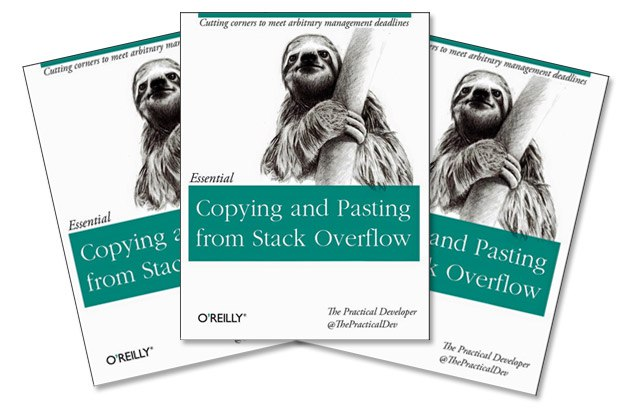
\includegraphics{images/2AmXWgVoULk.jpg}

Нет ничего постыдного в том, чтобы искать в Интернете решения проблем. Это абсолютно нормально. Используйте силу интернета во благо и да помогут Вам \emph{Stackoverflow} и бесчисленные R-туториалы!

Computer Programming To Be Officially Renamed ``Googling Stack Overflow''Source: http://t.co/xu7acfXvFF pic.twitter.com/iJ9k7aAVhd

--- Stack Exchange July 20, 2015

Главное, помните: загуглить работающий ответ всегда недостаточно. Надо понять, как и почему он работает. Иначе что-то обязательно пойдет не так.

Кроме того, правильно загуглить проблему --- не так уж и просто.

Does anyone ever get good at R or do they just get good at googling how to do things in R

--- 🔬🖤Lauren M. Seyler, Ph.D.❤️⚒ href=``\url{https://twitter.com/mousquemere/status/1125522375141883907?ref_src=twsrc\%5Etfw}''\textgreater May 6, 2019

Итак, с векторами мы более-менее разобрались. Помните, что вектора --- это один из краеугольных камней Вашей работы в R. Если Вы хорошо с ними разобрались, то дальше все будет довольно несложно. Тем не менее, вектора --- это не все. Есть еще два важных типа данных: списки (\textbf{list}) и матрицы (\textbf{matrix}). Их можно рассматривать как своеобразное ``расширение'' векторов, каждый в свою сторону. Ну а списки и матрицы нужны чтобы понять основной тип данных в R --- \textbf{data.frame}.

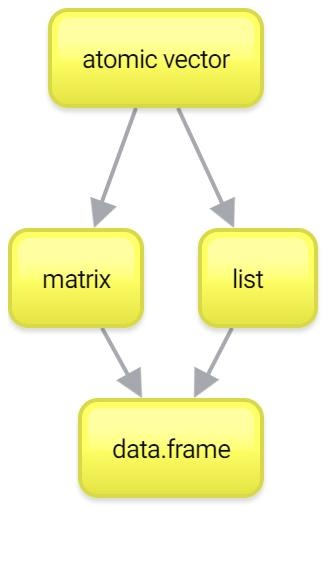
\includegraphics{images/New-Mind-Map.jpg}

\hypertarget{matrix}{%
\section{Матрицы (matrix)}\label{matrix}}

Если вдруг Вас пугает это слово, то совершенно зря. Матрица --- это всего лишь ``двумерный'' вектор: вектор, у которого есть не только длина, но и ширина. Создать матрицу можно с помощью функции \texttt{matrix()} из вектора, указав при этом количество строк и столбцов.

\begin{Shaded}
\begin{Highlighting}[]
\NormalTok{A <-}\StringTok{ }\KeywordTok{matrix}\NormalTok{(}\DecValTok{1}\OperatorTok{:}\DecValTok{20}\NormalTok{, }\DataTypeTok{nrow=}\DecValTok{5}\NormalTok{,}\DataTypeTok{ncol=}\DecValTok{4}\NormalTok{)}
\NormalTok{A}
\end{Highlighting}
\end{Shaded}

\begin{verbatim}
##      [,1] [,2] [,3] [,4]
## [1,]    1    6   11   16
## [2,]    2    7   12   17
## [3,]    3    8   13   18
## [4,]    4    9   14   19
## [5,]    5   10   15   20
\end{verbatim}

Если мы знаем сколько значений в матрице и сколько мы хотим строк, то количество столбцов указывать необязательно:

\begin{Shaded}
\begin{Highlighting}[]
\NormalTok{A <-}\StringTok{ }\KeywordTok{matrix}\NormalTok{(}\DecValTok{1}\OperatorTok{:}\DecValTok{20}\NormalTok{, }\DataTypeTok{nrow=}\DecValTok{5}\NormalTok{)}
\NormalTok{A}
\end{Highlighting}
\end{Shaded}

\begin{verbatim}
##      [,1] [,2] [,3] [,4]
## [1,]    1    6   11   16
## [2,]    2    7   12   17
## [3,]    3    8   13   18
## [4,]    4    9   14   19
## [5,]    5   10   15   20
\end{verbatim}

Все остальное так же как и с векторами: внутри находится данные только одного типа. Поскольку матрица --- это уже двумерный массив, то у него имеется два индекса. Эти два индекса разделяются запятыми.

\begin{Shaded}
\begin{Highlighting}[]
\NormalTok{A[}\DecValTok{2}\NormalTok{,}\DecValTok{3}\NormalTok{]}
\end{Highlighting}
\end{Shaded}

\begin{verbatim}
## [1] 12
\end{verbatim}

\begin{Shaded}
\begin{Highlighting}[]
\NormalTok{A[}\DecValTok{2}\OperatorTok{:}\DecValTok{4}\NormalTok{, }\DecValTok{1}\OperatorTok{:}\DecValTok{3}\NormalTok{]}
\end{Highlighting}
\end{Shaded}

\begin{verbatim}
##      [,1] [,2] [,3]
## [1,]    2    7   12
## [2,]    3    8   13
## [3,]    4    9   14
\end{verbatim}

Первый индекс --- выбор строк, второй индекс --- выбор колонок. Если же мы оставляем пустое поле вместо числа, то мы выбираем все строки/колонки в зависимости от того, оставили мы поле пустым до или после запятой:

\begin{Shaded}
\begin{Highlighting}[]
\NormalTok{A[,}\DecValTok{1}\OperatorTok{:}\DecValTok{3}\NormalTok{]}
\end{Highlighting}
\end{Shaded}

\begin{verbatim}
##      [,1] [,2] [,3]
## [1,]    1    6   11
## [2,]    2    7   12
## [3,]    3    8   13
## [4,]    4    9   14
## [5,]    5   10   15
\end{verbatim}

\begin{Shaded}
\begin{Highlighting}[]
\NormalTok{A[}\DecValTok{2}\OperatorTok{:}\DecValTok{4}\NormalTok{,]}
\end{Highlighting}
\end{Shaded}

\begin{verbatim}
##      [,1] [,2] [,3] [,4]
## [1,]    2    7   12   17
## [2,]    3    8   13   18
## [3,]    4    9   14   19
\end{verbatim}

\begin{Shaded}
\begin{Highlighting}[]
\NormalTok{A[,]}
\end{Highlighting}
\end{Shaded}

\begin{verbatim}
##      [,1] [,2] [,3] [,4]
## [1,]    1    6   11   16
## [2,]    2    7   12   17
## [3,]    3    8   13   18
## [4,]    4    9   14   19
## [5,]    5   10   15   20
\end{verbatim}

В принципе, это все, что нам нужно знать о матрицах. Матрицы используются в R довольно редко, особенно по сравнению, например, с MATLAB. Но вот индексировать матрицы хорошо бы уметь: это понадобится в работе с датафреймами.

\begin{quote}
То, что матрица - это просто двумерный вектор, не является метафорой: в R матрица - это по сути своей вектор с дополнительными \emph{атрибутами} \texttt{dim} и \texttt{dimnames}. Атрибуты --- это неотъемлемые свойства объектов, для всех объектов есть обязательные атрибуты типа и длины и могут быть любые необязательные атрибуты. Можно задавать свои атрибуты или удалять уже присвоенные: удаление атрибута \texttt{dim} у матрицы превратит ее в обычный вектор. Про атрибуты подробнее можно почитать \href{https://perso.esiee.fr/~courivad/R/06-objects.html}{здесь} или на стр. 99--101 книги ``R in a Nutshell'' \citep{adler2010r}.
\end{quote}

\hypertarget{list}{%
\section{Списки (list)}\label{list}}

Теперь представим себе вектор без ограничения на одинаковые данные внутри. И получим список!

\begin{Shaded}
\begin{Highlighting}[]
\NormalTok{l <-}\StringTok{ }\KeywordTok{list}\NormalTok{(}\DecValTok{42}\NormalTok{, }\StringTok{"Пам пам"}\NormalTok{, }\OtherTok{TRUE}\NormalTok{)}
\NormalTok{l}
\end{Highlighting}
\end{Shaded}

\begin{verbatim}
## [[1]]
## [1] 42
## 
## [[2]]
## [1] "Пам пам"
## 
## [[3]]
## [1] TRUE
\end{verbatim}

А это значит, что там могут содержаться самые разные данные, в том числе и другие списки и векторы!

\begin{Shaded}
\begin{Highlighting}[]
\NormalTok{lbig <-}\StringTok{ }\KeywordTok{list}\NormalTok{(}\KeywordTok{c}\NormalTok{(}\StringTok{"Wow"}\NormalTok{, }\StringTok{"this"}\NormalTok{, }\StringTok{"list"}\NormalTok{, }\StringTok{"is"}\NormalTok{, }\StringTok{"so"}\NormalTok{, }\StringTok{"big"}\NormalTok{), }\StringTok{"16"}\NormalTok{, l)}
\NormalTok{lbig}
\end{Highlighting}
\end{Shaded}

\begin{verbatim}
## [[1]]
## [1] "Wow"  "this" "list" "is"   "so"   "big" 
## 
## [[2]]
## [1] "16"
## 
## [[3]]
## [[3]][[1]]
## [1] 42
## 
## [[3]][[2]]
## [1] "Пам пам"
## 
## [[3]][[3]]
## [1] TRUE
\end{verbatim}

Если у нас сложный список, то есть очень классная функция, чтобы посмотреть, как он устроен, под названием \texttt{str()}:

\begin{Shaded}
\begin{Highlighting}[]
\KeywordTok{str}\NormalTok{(lbig)}
\end{Highlighting}
\end{Shaded}

\begin{verbatim}
## List of 3
##  $ : chr [1:6] "Wow" "this" "list" "is" ...
##  $ : chr "16"
##  $ :List of 3
##   ..$ : num 42
##   ..$ : chr "Пам пам"
##   ..$ : logi TRUE
\end{verbatim}

Как и в случае с векторами мы можем давать имена элементам списка:

\begin{Shaded}
\begin{Highlighting}[]
\NormalTok{namedl <-}\StringTok{ }\KeywordTok{list}\NormalTok{(}\DataTypeTok{age =} \DecValTok{24}\NormalTok{, }\DataTypeTok{PhDstudent =}\NormalTok{ T, }\DataTypeTok{language =} \StringTok{"Russian"}\NormalTok{)}
\NormalTok{namedl}
\end{Highlighting}
\end{Shaded}

\begin{verbatim}
## $age
## [1] 24
## 
## $PhDstudent
## [1] FALSE
## 
## $language
## [1] "Russian"
\end{verbatim}

К списку можно обращаться как с помощью индексов, так и по именам. Начнем с последнего:

\begin{Shaded}
\begin{Highlighting}[]
\NormalTok{namedl}\OperatorTok{$}\NormalTok{age}
\end{Highlighting}
\end{Shaded}

\begin{verbatim}
## [1] 24
\end{verbatim}

А вот с индексами сложнее, и в этом очень легко запутаться. Давайте попробуем сделать так, как мы делали это раньше:

\begin{Shaded}
\begin{Highlighting}[]
\NormalTok{namedl[}\DecValTok{1}\NormalTok{]}
\end{Highlighting}
\end{Shaded}

\begin{verbatim}
## $age
## [1] 24
\end{verbatim}

Мы, по сути, получили элемент списка - просто как часть списка, т.е. как список длиной один:

\begin{Shaded}
\begin{Highlighting}[]
\KeywordTok{class}\NormalTok{(namedl)}
\end{Highlighting}
\end{Shaded}

\begin{verbatim}
## [1] "list"
\end{verbatim}

\begin{Shaded}
\begin{Highlighting}[]
\KeywordTok{class}\NormalTok{(namedl[}\DecValTok{1}\NormalTok{])}
\end{Highlighting}
\end{Shaded}

\begin{verbatim}
## [1] "list"
\end{verbatim}

А вот чтобы добраться до самого элемента списка (и сделать с ним что-то хорошее) нам нужна не одна, а две квадратных скобочки:

\begin{Shaded}
\begin{Highlighting}[]
\NormalTok{namedl[[}\DecValTok{1}\NormalTok{]]}
\end{Highlighting}
\end{Shaded}

\begin{verbatim}
## [1] 24
\end{verbatim}

\begin{Shaded}
\begin{Highlighting}[]
\KeywordTok{class}\NormalTok{(namedl[[}\DecValTok{1}\NormalTok{]])}
\end{Highlighting}
\end{Shaded}

\begin{verbatim}
## [1] "numeric"
\end{verbatim}

Indexing lists in \#rstats. Inspired by the Residence Inn pic.twitter.com/YQ6axb2w7t

--- Hadley Wickham (@ href=``\url{https://twitter.com/hadleywickham/status/643381054758363136?ref_src=twsrc\%5Etfw}''\textgreater September 14, 2015

Как и в случае с вектором, к элементу списка можно обращаться по имени.

\begin{Shaded}
\begin{Highlighting}[]
\NormalTok{namedl[[}\StringTok{'age'}\NormalTok{]]}
\end{Highlighting}
\end{Shaded}

\begin{verbatim}
## [1] 24
\end{verbatim}

Хотя последнее --- практически то же самое, что и использование знака \$.

\begin{quote}
Списки довольно часто используются в R, но реже, чем в Python. Со многими объектами в R, такими как результаты статистических тестов, объекты ggplot и т.д. удобно работать именно как со списками --- к ним все вышеописанное применимо. Кроме того, некоторые данные мы изначально получаем в виде древообразной структуры --- хочешь не хочешь, а придется работать с этим как со списком. Но обычно после этого стоит как можно скорее превратить список в датафрейм.
\end{quote}

\hypertarget{df}{%
\section{Data.frame}\label{df}}

Итак, мы перешли к самому главному. Самому-самому. Датафреймы (\textbf{data.frames}). Более того, сейчас станет понятно, зачем нам нужно было разбираться со всеми предыдущими темами.

Без векторов мы не смогли бы разобраться с матрицами и списками. А без последних мы не сможем понять, что такое датафрейм.

\begin{Shaded}
\begin{Highlighting}[]
\NormalTok{name <-}\StringTok{ }\KeywordTok{c}\NormalTok{(}\StringTok{"Ivan"}\NormalTok{, }\StringTok{"Eugeny"}\NormalTok{, }\StringTok{"Lena"}\NormalTok{, }\StringTok{"Misha"}\NormalTok{, }\StringTok{"Sasha"}\NormalTok{) }
\NormalTok{age <-}\StringTok{ }\KeywordTok{c}\NormalTok{(}\DecValTok{26}\NormalTok{, }\DecValTok{34}\NormalTok{, }\DecValTok{23}\NormalTok{, }\DecValTok{27}\NormalTok{, }\DecValTok{26}\NormalTok{) }
\NormalTok{student <-}\StringTok{ }\KeywordTok{c}\NormalTok{(}\OtherTok{FALSE}\NormalTok{, }\OtherTok{FALSE}\NormalTok{, }\OtherTok{TRUE}\NormalTok{, }\OtherTok{TRUE}\NormalTok{, }\OtherTok{TRUE}\NormalTok{) }
\NormalTok{df =}\StringTok{ }\KeywordTok{data.frame}\NormalTok{(name, age, student)  }
\NormalTok{df}
\end{Highlighting}
\end{Shaded}

\begin{verbatim}
##     name age student
## 1   Ivan  26   FALSE
## 2 Eugeny  34   FALSE
## 3   Lena  23    TRUE
## 4  Misha  27    TRUE
## 5  Sasha  26    TRUE
\end{verbatim}

\begin{Shaded}
\begin{Highlighting}[]
\KeywordTok{str}\NormalTok{(df)}
\end{Highlighting}
\end{Shaded}

\begin{verbatim}
## 'data.frame':    5 obs. of  3 variables:
##  $ name   : Factor w/ 5 levels "Eugeny","Ivan",..: 2 1 3 4 5
##  $ age    : num  26 34 23 27 26
##  $ student: logi  FALSE FALSE TRUE TRUE TRUE
\end{verbatim}

Вообще, очень похоже на список, не правда ли? Так и есть, датафрейм --- это что-то вроде проименованного списка, каждый элемент которого является atomic вектором фиксированной длины. Скорее всего, список Вы представляли ``горизонтально''. Если это так, то теперь ``переверните'' его у себя в голове. Так, чтоб названия векторов оказались сверху, а колонки стали столбцами. Поскольку длина всех этих векторов равна (обязательное условие!), то данные представляют собой табличку, похожую на матрицу. Но в отличие от матрицы, разные столбцы могут имет разные типы данных: первая колонка --- character, вторая колонка --- numeric, третья колонка --- logical. Тем не менее, обращаться с датафреймом можно и как с проименованным списком, и как с матрицей:

\begin{Shaded}
\begin{Highlighting}[]
\NormalTok{df}\OperatorTok{$}\NormalTok{age[}\DecValTok{2}\OperatorTok{:}\DecValTok{3}\NormalTok{]}
\end{Highlighting}
\end{Shaded}

\begin{verbatim}
## [1] 34 23
\end{verbatim}

Здесь мы сначала вытащили колонку \texttt{age} с помощью оператора \texttt{\$}. Результатом этой операции является числовой вектор, из которого мы вытащили кусок, выбрав индексы \texttt{2} и \texttt{3}.

Используя оператор \texttt{\$} и присваивание можно создавать новые колонки датафрейма:

\begin{Shaded}
\begin{Highlighting}[]
\NormalTok{df}\OperatorTok{$}\NormalTok{lovesR <-}\StringTok{ }\OtherTok{TRUE} \CommentTok{#правило recycling - узнали? }
\NormalTok{df}
\end{Highlighting}
\end{Shaded}

\begin{verbatim}
##     name age student lovesR
## 1   Ivan  26   FALSE   TRUE
## 2 Eugeny  34   FALSE   TRUE
## 3   Lena  23    TRUE   TRUE
## 4  Misha  27    TRUE   TRUE
## 5  Sasha  26    TRUE   TRUE
\end{verbatim}

Ну а можно просто обращаться с помощью двух индексов через запятую, как мы это делали с матрицей:

\begin{Shaded}
\begin{Highlighting}[]
\NormalTok{df[}\DecValTok{3}\OperatorTok{:}\DecValTok{5}\NormalTok{, }\DecValTok{2}\OperatorTok{:}\DecValTok{3}\NormalTok{]}
\end{Highlighting}
\end{Shaded}

\begin{verbatim}
##   age student
## 3  23    TRUE
## 4  27    TRUE
## 5  26    TRUE
\end{verbatim}

Как и с матрицами, первый индекс означает строчки, а второй --- столбцы.

А еще можно использовать названия колонок внутри квадратных скобок:

\begin{Shaded}
\begin{Highlighting}[]
\NormalTok{df[}\DecValTok{1}\OperatorTok{:}\DecValTok{2}\NormalTok{,}\StringTok{"age"}\NormalTok{]}
\end{Highlighting}
\end{Shaded}

\begin{verbatim}
## [1] 26 34
\end{verbatim}

И здесь перед нами открываются невообразимые возможности! Узнаем, любят ли R те, кто моложе среднего возраста в группе:

\begin{Shaded}
\begin{Highlighting}[]
\NormalTok{df[df}\OperatorTok{$}\NormalTok{age }\OperatorTok{<}\StringTok{ }\KeywordTok{mean}\NormalTok{(df}\OperatorTok{$}\NormalTok{age), }\DecValTok{4}\NormalTok{]}
\end{Highlighting}
\end{Shaded}

\begin{verbatim}
## [1] TRUE TRUE TRUE TRUE
\end{verbatim}

Эту же задачу можно выполнить другими способами:

\begin{Shaded}
\begin{Highlighting}[]
\NormalTok{df}\OperatorTok{$}\NormalTok{lovesR[df}\OperatorTok{$}\NormalTok{age }\OperatorTok{<}\StringTok{ }\KeywordTok{mean}\NormalTok{(df}\OperatorTok{$}\NormalTok{age)]}
\end{Highlighting}
\end{Shaded}

\begin{verbatim}
## [1] TRUE TRUE TRUE TRUE
\end{verbatim}

\begin{Shaded}
\begin{Highlighting}[]
\NormalTok{df[df}\OperatorTok{$}\NormalTok{age }\OperatorTok{<}\StringTok{ }\KeywordTok{mean}\NormalTok{(df}\OperatorTok{$}\NormalTok{age), }\StringTok{'lovesR'}\NormalTok{]}
\end{Highlighting}
\end{Shaded}

\begin{verbatim}
## [1] TRUE TRUE TRUE TRUE
\end{verbatim}

В большинстве случаев подходят сразу несколько способов --- тем не менее, стоит овладеть ими всеми.

Датафреймы удобно просматривать в RStudio. Для это нужно написать команду \texttt{View(df)} или же просто нажать на названии нужной переменной из списка вверху справа (там где Environment). Тогда увидите табличку, очень похожую на Excel и тому подобные программы для работы с таблицами. Там же есть и всякие возможности для фильтрации, сортировки и поиска\ldots{} Но, конечно, интереснее все эти вещи делать руками, т.е. с помощью написания кода.

На этом пора заканчивать с введением и приступать к реальным данным.

\hypertarget{real_data}{%
\section{Начинаем работу с реальными данными}\label{real_data}}

Итак, пришло время перейти к реальным данным. Мы начнем с использования датасета (так мы будем называть любой набор данных) по Игре Престолов, а точнее, по книгам цикла \emph{``Песнь льда и пламени''} Дж. Мартина. Да, будут спойлеры, но сериал уже давно закончился и сильно разошелся с книгами\ldots{}

\hypertarget{wd}{%
\subsection{Рабочая папка и проекты}\label{wd}}

Для начала скачайте файл по \href{https://raw.githubusercontent.com/Pozdniakov/stats/master/data/character-deaths.csv}{ссылке}

Он, скорее всего, появился у Вас в папке ``Загрузки''. Если мы будем просто пытаться прочитать этот файл (например, с помощью \texttt{read.csv()} --- мы к этой функцией очень скоро перейдем), указав его имя и разрешение, то наткнемся на такую ошибку:

\begin{quote}
Ошибка в file(file, ``rt'') :не могу открыть соединение
Вдобавок: Предупреждение:
В file(file, ``rt'') :
не могу открыть файл `character-deaths.csv': No such file or directory
\end{quote}

Это означает, что R не может найти нужный файл. Вообще-то мы даже не сказали, где искать. Нам нужно как-то совместить место, где R ищет загружаемые файлы и сами файлы. Для этого есть несколько способов.

\begin{itemize}
\tightlist
\item
  Магомет идет к горе: перемещение файлов в рабочую папку.
\end{itemize}

Для этого нужно узнать, какая папка является рабочей с помощью функции \texttt{getwd()} (без аргументов), найти эту папку в проводнике и переместить туда файл. После этого можно использовать просто название файла с разрешением:

\begin{Shaded}
\begin{Highlighting}[]
\NormalTok{got <-}\StringTok{ }\KeywordTok{read.csv}\NormalTok{(}\StringTok{"character-deaths.csv"}\NormalTok{)}
\end{Highlighting}
\end{Shaded}

\begin{itemize}
\tightlist
\item
  Гора идет к Магомету: изменение рабочей папки.
\end{itemize}

Можно просто сменить рабочую папку с помощью \texttt{setwd()} на ту, где сейчас лежит файл, прописав путь до этой папки. Теперь файл находится в рабочей папке:

\begin{Shaded}
\begin{Highlighting}[]
\NormalTok{got <-}\StringTok{ }\KeywordTok{read.csv}\NormalTok{(}\StringTok{"character-deaths.csv"}\NormalTok{)}
\end{Highlighting}
\end{Shaded}

Этот вариант использовать не рекомендуется. Как минимум, это сразу делает невозможным запустить скрипт на другом компьютере.

\begin{itemize}
\tightlist
\item
  Гора находит Магомета по месту прописки: указание полного пути файла.
\end{itemize}

\begin{Shaded}
\begin{Highlighting}[]
\NormalTok{got <-}\StringTok{ }\KeywordTok{read.csv}\NormalTok{(}\StringTok{"/Users/Username/Some_Folder/character-deaths.csv"}\NormalTok{)}
\end{Highlighting}
\end{Shaded}

Этот вариант страдает теми же проблемами, что и предыдущий, поэтому тоже не рекомендуется.

\begin{quote}
Для пользователей Windows есть дополнительная сложность: знак \texttt{/} является особым знаком для R, поэтому вместо него нужно использовать двойной \texttt{//}.
\end{quote}

\begin{itemize}
\tightlist
\item
  Магомет использует кнопочный интерфейс: Import Dataset.
\end{itemize}

Во вкладке Environment справа в окне RStudio есть кнопка ``Import Dataset''. Возможно, у Вас возникло непреодолимое желание отдохнуть от написания кода и понажимать кнопочки --- сопротивляйтесь этому всеми силами, но не вините себя, если не сдержитесь.

\begin{itemize}
\tightlist
\item
  Гора находит Магомета в интернете.
\end{itemize}

Многие функции в R, предназначенные для чтения файлов, могут прочитать файл не только на Вашем компьютере, но и сразу из интернета. Для этого просто используйте ссылку вместо пути:

\begin{Shaded}
\begin{Highlighting}[]
\NormalTok{got <-}\StringTok{ }\KeywordTok{read.csv}\NormalTok{(}\StringTok{"https://raw.githubusercontent.com/Pozdniakov/stats/master/data/character-deaths.csv"}\NormalTok{)}
\end{Highlighting}
\end{Shaded}

\begin{itemize}
\tightlist
\item
  Каждый Магомет получает по своей горе: использование проектов в RStudio.
\end{itemize}

На первый взгляд это кажется чем-то очень сложным, но это не так. Это очень просто и ОЧЕНЬ удобно. При создании проекта создается отдельная папочка, где у Вас лежат данные, хранятся скрипты, вспомогательные файлы и отчеты. Если нужно вернуться к другому проекту --- просто открываете другой проект, с другими файлами и скриптами. Это еще помогает не пересекаться переменным из разных проектов --- а то, знаете, использование двух переменных \texttt{data} в разных скриптах чревато ошибками. Поэтому очень удобным решением будет выделение отдельного проекта под этот курс.

\hypertarget{import}{%
\subsection{Импорт данных}\label{import}}

Как Вы уже поняли, импортирование данных - одна из самых муторных и неприятных вещей в R. Если у Вас получится с этим справится, то все остальное - ерунда. Мы уже разобрались с первой частью этого процесса - нахождением файла с данными, осталось научиться их читать.

Здесь стоит сделать небольшую ремарку. Довольно часто данные представляют собой табличку. Или же их можно свести к табличке. Такая табличка, как мы уже выяснили, удобно репрезентируется в виде датафрейма. Но как эти данные хранятся на компьютере? Есть два варианта: в \emph{бинарном} и в \emph{текстовом} файле.

Текстовый файл означает, что такой файл можно открыть в программе ``Блокнот'' или ее аналоге и увидеть напечатанный текст: скрипт, роман или упорядоченный набор цифр и букв. Нас сейчас интересует именно последний случай. Таблица может быть представлена как текст: отдельные строчки в файле будут разделять разные строчки таблицы, а какой-нибудь знак-разделитель отделет колонки друг от друга.

Для чтения данных из текстового файла есть довольно удобная функция \texttt{read.table()}. Почитайте хэлп по ней и ужаснитесь: столько разных параметров на входе! Но там же вы увидете функции \texttt{read.csv()}, \texttt{read.csv2()} и некоторые другие --- по сути, это тот же \texttt{read.table()}, но с другими дефолтными параметрами, соответствующие формату файла, который мы загружаем. В данном случае используется формат .csv, что означает Comma Separated Values (Значения, Разделенные Запятыми). Это просто текстовый файл, в котором ``закодирована'' таблица: разные строчки разделяют разные строчки таблицы, а столбцы отделяются запятыми. С этим связана одна проблема: в некоторых странах (в т.ч. и России) принято использовать запятую для разделения дробной части числа, а не точку, как это делается в большинстве стран мира. Поэтому есть ``другой'' формат .csv, где значения разделены точкой с запятой (\texttt{;}), а дробные значения - запятой (\texttt{,}). В этом и различие функций \texttt{read.csv()} и \texttt{read.csv2()} --- первая функция предназначена для ``международного'' формата, вторая - для (условно) ``Российского''.

В первой строчке обычно содержатся названия столбцов - и это чертовски удобно, функции \texttt{read.csv()} и \texttt{read.csv2()} по дефолту считают первую строчку именно как название для колонок.

Итак, прочитаем наш файл. Для этого используем только параметр \texttt{file\ =}, который идет первым, и для параметра \texttt{stringsAsFactors\ =} поставим значение \texttt{FALSE}:

\begin{Shaded}
\begin{Highlighting}[]
\NormalTok{got <-}\StringTok{ }\KeywordTok{read.csv}\NormalTok{(}\StringTok{"data/character-deaths.csv"}\NormalTok{, }\DataTypeTok{stringsAsFactors =} \OtherTok{FALSE}\NormalTok{)}
\end{Highlighting}
\end{Shaded}

\begin{quote}
По сути, факторы - это примерно то же самое, что и character, но закодированные числами. Когда-то это было придумано для экономии используемых времени и памяти, сейчас же обычно становится просто лишней морокой. Но некоторые функции требуют именно character, некоторые factor, в большинстве случаев это без разницы. Но иногда непонимание может привести к дурацким ошибкам. В данном случае мы просто пока обойдемся без факторов.
\end{quote}

Можете проверить с помощью \texttt{View(got)}: все работает! Если же вылезает какая-то странная ерунда или же просто ошибка - попробуйте другие функции и покопаться с параметрами. Для этого читайте Help.

Кроме .csv формата есть и другие варианты хранения таблиц в виде текста. Например, .tsv
- тоже самое, что и .csv, но разделитель - знак табуляции. Для чтения таких файлов есть функция \texttt{read.delim()} и \texttt{read.delim2()}. Впрочем, даже если бы ее и не было, можно было бы просто подобрать нужные параметры для функции \texttt{read.table()}. Есть даже функции, которые пытаются сами ``угадать'' нужные параметры для чтения --- часто они справляются с этим довольно удачно. Но не всегда. Поэтому стоит научиться справляться с любого рода данными на входе.

Тем не менее, далеко не всегда таблицы представлены в виде текстового файла. Самый распространенный пример таблицы в бинарном виде --- родные форматы Microsoft Excel. Если Вы попробуете открыть .xlsx файл в Блокноте, то увидите кракозябры. Это делает работу с этим файлами гораздо менее удобной, поэтому стоит избегать экселевских форматов и стараться все сохранять в .csv.

\begin{quote}
Для работы с экселевскими файлами есть много пакетов: readxl, xlsx, openxlsx. Для чтения файлов SPSS, Stata, SAS есть пакет foreign. Что такое пакеты и как их устанавливать мы изучим позже.
\end{quote}

\hypertarget{prep}{%
\section{Препроцессинг данных в R}\label{prep}}

Вчера мы узнали про основы языка R, про то, как работать с векторами, списками, матрицами и, наконец, датафреймами. Мы закончили день на загрузке данных, с чего мы и начнем сегодня:

\begin{Shaded}
\begin{Highlighting}[]
\NormalTok{got <-}\StringTok{ }\KeywordTok{read.csv}\NormalTok{(}\StringTok{"data/character-deaths.csv"}\NormalTok{, }\DataTypeTok{stringsAsFactors =}\NormalTok{ F)}
\end{Highlighting}
\end{Shaded}

После загрузки данных стоит немного ``осмотреть'' получившийся датафрейм \texttt{got}.

\hypertarget{explore}{%
\subsection{Исследование данных}\label{explore}}

Ок, давайте немного поизучаем датасет. Обычно мы привыкли глазами пробегать по данным, листая строки и столбцы --- и это вполне правильно и логично, от этого не нужно отучаться. Но мы можем дополнить наш базовый зрительнопоисковой инструментарий несколькими полезными командами.

Во-первых, вспомним другую полезную функцию \texttt{str()}:

\begin{Shaded}
\begin{Highlighting}[]
\KeywordTok{str}\NormalTok{(got)}
\end{Highlighting}
\end{Shaded}

\begin{verbatim}
## 'data.frame':    917 obs. of  13 variables:
##  $ Name              : chr  "Addam Marbrand" "Aegon Frey (Jinglebell)" "Aegon Targaryen" "Adrack Humble" ...
##  $ Allegiances       : chr  "Lannister" "None" "House Targaryen" "House Greyjoy" ...
##  $ Death.Year        : int  NA 299 NA 300 NA NA 300 300 NA NA ...
##  $ Book.of.Death     : int  NA 3 NA 5 NA NA 4 5 NA NA ...
##  $ Death.Chapter     : int  NA 51 NA 20 NA NA 35 NA NA NA ...
##  $ Book.Intro.Chapter: int  56 49 5 20 NA NA 21 59 11 0 ...
##  $ Gender            : int  1 1 1 1 1 1 1 0 1 1 ...
##  $ Nobility          : int  1 1 1 1 1 1 1 1 1 0 ...
##  $ GoT               : int  1 0 0 0 0 0 1 1 0 0 ...
##  $ CoK               : int  1 0 0 0 0 1 0 1 1 0 ...
##  $ SoS               : int  1 1 0 0 1 1 1 1 0 1 ...
##  $ FfC               : int  1 0 0 0 0 0 1 0 1 0 ...
##  $ DwD               : int  0 0 1 1 0 0 0 1 0 0 ...
\end{verbatim}

Давайте разберемся с переменными в датафрейме:

Колонка \texttt{Name} --- здесь все понятно. Важно, что эти имена записаны абсолютно по-разному: где-то с фамилией, где-то без, где-то в скобочках есть пояснения. Колонка \texttt{Allegiances} --- к какому дому принадлежит персонаж. С этим сложно, иногда они меняют дома, здесь путаются сами семьи и персонажи, лояльные им. Особой разницы между \texttt{Stark} и \texttt{House\ Stark} нет. Следующие колонки - \texttt{Death\ Year}, \texttt{Book.of.Death}, \texttt{Death.Chapter}, \texttt{Book.Intro.Chapter} --- означают номер главы, в которой персонаж впервые появляется, а так же номер книги, глава и год (от завоевания Вестероса Эйгоном Таргариеном), в которой персонаж умирает. \texttt{Gender} --- \texttt{1} для мужчин, \texttt{0} для женщин. \texttt{Nobility} --- дворянское происхождение персонажа. Последние 5 столбцов содержат информацию, появлялся ли персонаж в книге (всего книг пока что 5).

Другая полезная функция для больших таблиц --- функция \texttt{head()}: она выведет первые несколько (по дефолту 6) строчек датафрейма.

\begin{Shaded}
\begin{Highlighting}[]
\KeywordTok{head}\NormalTok{(got)}
\end{Highlighting}
\end{Shaded}

\begin{verbatim}
##                      Name     Allegiances Death.Year Book.of.Death
## 1          Addam Marbrand       Lannister         NA            NA
## 2 Aegon Frey (Jinglebell)            None        299             3
## 3         Aegon Targaryen House Targaryen         NA            NA
## 4           Adrack Humble   House Greyjoy        300             5
## 5          Aemon Costayne       Lannister         NA            NA
## 6         Aemon Estermont       Baratheon         NA            NA
##   Death.Chapter Book.Intro.Chapter Gender Nobility GoT CoK SoS FfC DwD
## 1            NA                 56      1        1   1   1   1   1   0
## 2            51                 49      1        1   0   0   1   0   0
## 3            NA                  5      1        1   0   0   0   0   1
## 4            20                 20      1        1   0   0   0   0   1
## 5            NA                 NA      1        1   0   0   1   0   0
## 6            NA                 NA      1        1   0   1   1   0   0
\end{verbatim}

Есть еще функция \texttt{tail()}. Догадайтесь сами, что она делает.

Для некоторых переменных полезно посмотреть таблицы частотности с помощью функции table():

\begin{Shaded}
\begin{Highlighting}[]
\KeywordTok{table}\NormalTok{(got}\OperatorTok{$}\NormalTok{Allegiances)}
\end{Highlighting}
\end{Shaded}

\begin{verbatim}
## 
##           Arryn       Baratheon         Greyjoy     House Arryn 
##              23              56              51               7 
## House Baratheon   House Greyjoy House Lannister   House Martell 
##               8              24              21              12 
##     House Stark House Targaryen     House Tully    House Tyrell 
##              35              19               8              11 
##       Lannister         Martell   Night's Watch            None 
##              81              25             116             253 
##           Stark       Targaryen           Tully          Tyrell 
##              73              17              22              15 
##        Wildling 
##              40
\end{verbatim}

Уау! Очень просто и удобно, не так ли? Функция \texttt{table()} может принимать сразу несколько столбцов. Это удобно для получения \emph{таблиц сопряженности}:

\begin{Shaded}
\begin{Highlighting}[]
\KeywordTok{table}\NormalTok{(got}\OperatorTok{$}\NormalTok{Allegiances, got}\OperatorTok{$}\NormalTok{Gender)}
\end{Highlighting}
\end{Shaded}

\begin{verbatim}
##                  
##                     0   1
##   Arryn             3  20
##   Baratheon         6  50
##   Greyjoy           4  47
##   House Arryn       3   4
##   House Baratheon   0   8
##   House Greyjoy     1  23
##   House Lannister   2  19
##   House Martell     7   5
##   House Stark       6  29
##   House Targaryen   5  14
##   House Tully       0   8
##   House Tyrell      4   7
##   Lannister        12  69
##   Martell           7  18
##   Night's Watch     0 116
##   None             51 202
##   Stark            21  52
##   Targaryen         1  16
##   Tully             2  20
##   Tyrell            6   9
##   Wildling         16  24
\end{verbatim}

\hypertarget{subset}{%
\subsection{Subsetting}\label{subset}}

Как мы обсуждали на прошлом занятии, мы можем сабсеттить (выделять часть датафрейма) датафрейм, обращаясь к нему и как к матрице: \emph{датафрейм{[}вектор\_с\_номерами\_строк, вектор\_с\_номерами\_колонок{]}}

\begin{Shaded}
\begin{Highlighting}[]
\NormalTok{got[}\DecValTok{100}\OperatorTok{:}\DecValTok{115}\NormalTok{, }\DecValTok{1}\OperatorTok{:}\DecValTok{2}\NormalTok{]}
\end{Highlighting}
\end{Shaded}

\begin{verbatim}
##                 Name   Allegiances
## 100        Blue Bard  House Tyrell
## 101    Bonifer Hasty     Lannister
## 102           Borcas Night's Watch
## 103  Boremund Harlaw       Greyjoy
## 104     Boros Blount     Baratheon
## 105           Borroq      Wildling
## 106      Bowen Marsh Night's Watch
## 107       Bran Stark   House Stark
## 108   Brandon Norrey         Stark
## 109          Brenett          None
## 110 Brienne of Tarth         Stark
## 111            Bronn     Lannister
## 112    Brown Bernarr Night's Watch
## 113           Brusco          None
## 114   Bryan Fossoway     Baratheon
## 115      Bryce Caron     Baratheon
\end{verbatim}

и используя имена колонок:

\begin{Shaded}
\begin{Highlighting}[]
\NormalTok{got[}\DecValTok{508}\OperatorTok{:}\DecValTok{515}\NormalTok{, }\StringTok{"Name"}\NormalTok{]}
\end{Highlighting}
\end{Shaded}

\begin{verbatim}
## [1] "Mance Rayder"    "Mandon Moore"    "Maric Seaworth"  "Marei"          
## [5] "Margaery Tyrell" "Marillion"       "Maris"           "Marissa Frey"
\end{verbatim}

и даже используя вектора названий колонок!

\begin{Shaded}
\begin{Highlighting}[]
\NormalTok{got[}\DecValTok{508}\OperatorTok{:}\DecValTok{515}\NormalTok{, }\KeywordTok{c}\NormalTok{(}\StringTok{"Name"}\NormalTok{, }\StringTok{"Allegiances"}\NormalTok{, }\StringTok{"Gender"}\NormalTok{)]}
\end{Highlighting}
\end{Shaded}

\begin{verbatim}
##                Name     Allegiances Gender
## 508    Mance Rayder        Wildling      1
## 509    Mandon Moore       Baratheon      1
## 510  Maric Seaworth House Baratheon      1
## 511           Marei            None      0
## 512 Margaery Tyrell    House Tyrell      0
## 513       Marillion           Arryn      1
## 514           Maris        Wildling      0
## 515    Marissa Frey            None      0
\end{verbatim}

Мы можем вытаскивать отдельные колонки как векторы:

\begin{Shaded}
\begin{Highlighting}[]
\NormalTok{houses <-}\StringTok{ }\NormalTok{got}\OperatorTok{$}\NormalTok{Allegiances}
\KeywordTok{unique}\NormalTok{(houses) }\CommentTok{#посмотреть все уникальные значения --- почти как с помощью table()}
\end{Highlighting}
\end{Shaded}

\begin{verbatim}
##  [1] "Lannister"       "None"            "House Targaryen"
##  [4] "House Greyjoy"   "Baratheon"       "Night's Watch"  
##  [7] "Arryn"           "House Stark"     "House Tyrell"   
## [10] "Tyrell"          "Stark"           "Greyjoy"        
## [13] "House Lannister" "Martell"         "House Martell"  
## [16] "Wildling"        "Targaryen"       "House Arryn"    
## [19] "House Tully"     "Tully"           "House Baratheon"
\end{verbatim}

Итак, давайте решим нашу первую задачу --- вытащим в отдельный датасет всех представителей Ночного Дозора.
Для этого нам нужно создать вектор логических значений --- результат сравнений колонки \texttt{Allegiances} со значением \texttt{"Night\textquotesingle{}s\ Watch"} и использовать его как вектор индексов для датафрейма.

\begin{Shaded}
\begin{Highlighting}[]
\NormalTok{vectornight <-}\StringTok{ }\NormalTok{got}\OperatorTok{$}\NormalTok{Allegiances }\OperatorTok{==}\StringTok{ "Night's Watch"}
\KeywordTok{head}\NormalTok{(vectornight)}
\end{Highlighting}
\end{Shaded}

\begin{verbatim}
## [1] FALSE FALSE FALSE FALSE FALSE FALSE
\end{verbatim}

Теперь этот вектор с \texttt{TRUE} и \texttt{FALSE} нам надо использовать для индексирования строк. Но что со столбцами? Если мы хотем сохранить все столбцы, то после запятой внутри квадратных скобок нам не нужно ничего указывать:

\begin{Shaded}
\begin{Highlighting}[]
\NormalTok{nightswatch <-}\StringTok{ }\NormalTok{got[vectornight,]}
\KeywordTok{head}\NormalTok{(nightswatch)}
\end{Highlighting}
\end{Shaded}

\begin{verbatim}
##                                 Name   Allegiances Death.Year
## 7  Aemon Targaryen (son of Maekar I) Night's Watch        300
## 10                            Aethan Night's Watch         NA
## 13                     Alan of Rosby Night's Watch        300
## 16                            Albett Night's Watch         NA
## 24                    Alliser Thorne Night's Watch         NA
## 49                             Arron Night's Watch         NA
##    Book.of.Death Death.Chapter Book.Intro.Chapter Gender Nobility GoT CoK
## 7              4            35                 21      1        1   1   0
## 10            NA            NA                  0      1        0   0   0
## 13             5             4                 18      1        1   0   1
## 16            NA            NA                 26      1        0   1   0
## 24            NA            NA                 19      1        0   1   1
## 49            NA            NA                 75      1        0   0   0
##    SoS FfC DwD
## 7    1   1   0
## 10   1   0   0
## 13   1   0   1
## 16   0   0   0
## 24   1   0   1
## 49   1   0   1
\end{verbatim}

Вуаля!
Все это можно сделать проще и в одну строку:

\begin{Shaded}
\begin{Highlighting}[]
\NormalTok{nightswatch <-}\StringTok{ }\NormalTok{got[got}\OperatorTok{$}\NormalTok{Allegiances }\OperatorTok{==}\StringTok{ "Night's Watch"}\NormalTok{,]}
\end{Highlighting}
\end{Shaded}

И не забывайте про запятую!

Теперь попробуем вытащить одновременно всех Одичалых (\texttt{Wildling}) и всех представителей Ночного Дозора. Это можно сделать, используя оператор \texttt{\textbar{}} (ИЛИ) при выборе колонок:

\begin{Shaded}
\begin{Highlighting}[]
\NormalTok{nightwatch_wildling <-}\StringTok{ }\NormalTok{got[got}\OperatorTok{$}\NormalTok{Allegiances }\OperatorTok{==}\StringTok{ "Night's Watch"} \OperatorTok{|}\StringTok{ }\NormalTok{got}\OperatorTok{$}\NormalTok{Allegiances }\OperatorTok{==}\StringTok{ "Wildling"}\NormalTok{,]}
\KeywordTok{head}\NormalTok{(nightwatch_wildling)}
\end{Highlighting}
\end{Shaded}

\begin{verbatim}
##                                 Name   Allegiances Death.Year
## 7  Aemon Targaryen (son of Maekar I) Night's Watch        300
## 10                            Aethan Night's Watch         NA
## 13                     Alan of Rosby Night's Watch        300
## 16                            Albett Night's Watch         NA
## 24                    Alliser Thorne Night's Watch         NA
## 49                             Arron Night's Watch         NA
##    Book.of.Death Death.Chapter Book.Intro.Chapter Gender Nobility GoT CoK
## 7              4            35                 21      1        1   1   0
## 10            NA            NA                  0      1        0   0   0
## 13             5             4                 18      1        1   0   1
## 16            NA            NA                 26      1        0   1   0
## 24            NA            NA                 19      1        0   1   1
## 49            NA            NA                 75      1        0   0   0
##    SoS FfC DwD
## 7    1   1   0
## 10   1   0   0
## 13   1   0   1
## 16   0   0   0
## 24   1   0   1
## 49   1   0   1
\end{verbatim}

\begin{quote}
Кажется очевидным следующий вариант: \texttt{got{[}got\$Allegiances\ ==\ c("Night\textquotesingle{}s\ Watch",\ "Wildling"),{]}}. Однако это выдаст не совсем то, что нужно, хотя результат может показаться верным на первый взгляд. Попробуйте самостоятельно ответить на вопрос, что происходит в данном случае и чем результат отличается от предполагаемого. Подсказка: вспомните правило recycling.
\end{quote}

Для таких случаев есть удобный оператор \texttt{\%in\%}, который позволяет сравнить каждое значение вектора с целым набором значений. Если значение вектора хотя бы один раз встречается в векторе справа от \texttt{\%in\%}, то результат --- \texttt{TRUE}:

\begin{Shaded}
\begin{Highlighting}[]
\DecValTok{1}\OperatorTok{:}\DecValTok{6} \OperatorTok\StringTok{ }\KeywordTok{c}\NormalTok{(}\DecValTok{1}\NormalTok{,}\DecValTok{4}\NormalTok{,}\DecValTok{5}\NormalTok{)}
\end{Highlighting}
\end{Shaded}

\begin{verbatim}
## [1]  TRUE FALSE FALSE  TRUE  TRUE FALSE
\end{verbatim}

\begin{Shaded}
\begin{Highlighting}[]
\NormalTok{nightwatch_wildling <-}\StringTok{ }\NormalTok{got[got}\OperatorTok{$}\NormalTok{Allegiances }\OperatorTok\StringTok{ }\KeywordTok{c}\NormalTok{(}\StringTok{"Night's Watch"}\NormalTok{, }\StringTok{"Wildling"}\NormalTok{),]}
\KeywordTok{head}\NormalTok{(nightwatch_wildling)}
\end{Highlighting}
\end{Shaded}

\begin{verbatim}
##                                 Name   Allegiances Death.Year
## 7  Aemon Targaryen (son of Maekar I) Night's Watch        300
## 10                            Aethan Night's Watch         NA
## 13                     Alan of Rosby Night's Watch        300
## 16                            Albett Night's Watch         NA
## 24                    Alliser Thorne Night's Watch         NA
## 49                             Arron Night's Watch         NA
##    Book.of.Death Death.Chapter Book.Intro.Chapter Gender Nobility GoT CoK
## 7              4            35                 21      1        1   1   0
## 10            NA            NA                  0      1        0   0   0
## 13             5             4                 18      1        1   0   1
## 16            NA            NA                 26      1        0   1   0
## 24            NA            NA                 19      1        0   1   1
## 49            NA            NA                 75      1        0   0   0
##    SoS FfC DwD
## 7    1   1   0
## 10   1   0   0
## 13   1   0   1
## 16   0   0   0
## 24   1   0   1
## 49   1   0   1
\end{verbatim}

\hypertarget{newcol}{%
\subsection{Создание новых колонок}\label{newcol}}

Давайте создадим новую колонку, которая будет означать, жив ли еще персонаж (по книгам).
Заметьте, что в этом датасете, хоть он и посвящен смертям персонажей, нет нужной колонки. Мы можем попытаться ``вытащить'' эту информацию. В колонках \texttt{Death.Year}, \texttt{Death.Chapter} и \texttt{Book.of.Death} стоит \texttt{NA} у многих персонажей. Например, у \texttt{Arya\ Stark}, которая и по книгам, и по сериалу живее всех живых и мертвых:

\begin{Shaded}
\begin{Highlighting}[]
\NormalTok{got[got}\OperatorTok{$}\NormalTok{Name }\OperatorTok{==}\StringTok{ "Arya Stark"}\NormalTok{,]}
\end{Highlighting}
\end{Shaded}

\begin{verbatim}
##          Name Allegiances Death.Year Book.of.Death Death.Chapter
## 56 Arya Stark       Stark         NA            NA            NA
##    Book.Intro.Chapter Gender Nobility GoT CoK SoS FfC DwD
## 56                  2      0        1   1   1   1   1   1
\end{verbatim}

Следовательно, если в \texttt{Book.of.Death} стоит \texttt{NA}, мы можем предположить, что Джордж Мартин еще не занес своей карающей руки над этим героем.

Мы можем создать новую колонку \texttt{Is.Alive}:

\begin{Shaded}
\begin{Highlighting}[]
\NormalTok{got}\OperatorTok{$}\NormalTok{Is.Alive <-}\StringTok{ }\KeywordTok{is.na}\NormalTok{(got}\OperatorTok{$}\NormalTok{Book.of.Death)}
\end{Highlighting}
\end{Shaded}

\hypertarget{dtvstidy}{%
\subsection{data.table vs.~tidyverse}\label{dtvstidy}}

В принципе, с помощью базового R можно сделать все, что угодно. Однако базовые инструменты R --- не всегда самые удобные. Идея сделать работу с датафреймами в R еще быстрее и удобнее сподвигла разработчиков на создание новых инструментов --- \texttt{data.table} и \texttt{tidyverse} (\texttt{dplyr}). Это два конкурирующих подхода, которые сильно перерабатывают язык, хотя это по-прежнему все тот же R --- поэтому их еще называют ``диалектами'' R.

Оба подхода обладают своими преимуществами и недостатками, но на сегодняшний день \texttt{tidyverse} считается более популярным. Основное преимущество этого подхода --- в относительной легкости освоения. Обычно код, написанный в \texttt{tidyverse} можно примерно понять, даже не владея им.

Преимущество \texttt{data.table} --- в суровом лаконичном синтаксисе и наиболее эффективных алгоритмах. Последние обеспечивают очень серьезный прирост в скорости в работе с данными. Чтение файлов и манипуляция данными может быть на порядки быстрее, поэтому если Ваш датасет с трудом пролезает в оперативную память компьютера, а исполнение скрипта занимает длительное время - стоит задуматься о переходе на \texttt{data.table}.

Что из этого учить --- решать Вам, но знать оба совсем не обязательно: они решают те же самые задачи, просто совсем разными способами. За data.table --- скорость, за tidyverse - понятность синтаксиса. Очень советую почитать обсуждение на эту тему \href{https://stackoverflow.com/questions/21435339/data-table-vs-dplyr-can-one-do-something-well-the-other-cant-or-does-poorly}{здесь}.

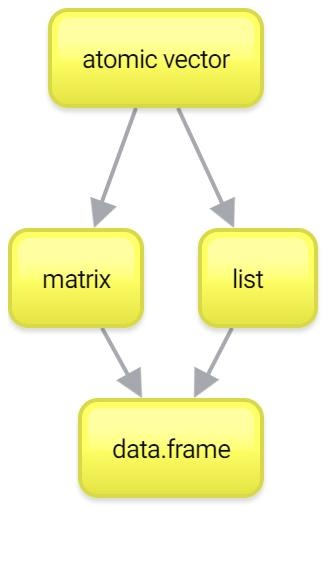
\includegraphics{images/New-Mind-Map.jpg}

\hypertarget{tidy_dplyr}{%
\chapter{\texorpdfstring{\texttt{tidyverse}: Загрузка и трансформация данных}{tidyverse: Загрузка и трансформация данных}}\label{tidy_dplyr}}

\href{https://www.tidyverse.org}{\emph{tidyverse}} --- это набор пакетов:

\begin{itemize}
\tightlist
\item
  \emph{ggplot2}, для визуализации
\item
  \emph{tibble}, для работы с тибблами, современный вариант датафрейма
\item
  \emph{tidyr}, для формата tidy data
\item
  \emph{readr}, для чтения файлов в R
\item
  \emph{purrr}, для функционального программирования
\item
  \emph{dplyr}, для преобразованиия данных
\item
  \emph{stringr}, для работы со строковыми переменными
\item
  \emph{forcats}, для работы с переменными-факторами
\end{itemize}

Полезно также знать о следующих:

\begin{itemize}
\tightlist
\item
  \emph{readxl}, для чтения .xls и .xlsx
\item
  \emph{jsonlite}, для работы с JSON
\item
  \emph{rvest}, для веб-скреппинга
\item
  \emph{lubridate}, для работы с временем
\item
  \emph{tidytext}, для работы с текстами и корпусами
\item
  \emph{broom}, для перевода в tidy формат статистические модели
\end{itemize}

\begin{Shaded}
\begin{Highlighting}[]
\KeywordTok{library}\NormalTok{(}\StringTok{"tidyverse"}\NormalTok{)}
\end{Highlighting}
\end{Shaded}

\hypertarget{section-3}{%
\section{Загрузка данных}\label{section-3}}

\hypertarget{section-4}{%
\subsection{Рабочая директория}\label{section-4}}

Все в R происходит где-то. Нужно загружать файлы с данными, нужно их куда-то сохранять. Желательно иметь для каждого проекта некоторую отдельную папку на компьютере, куда складывать все, отнсящееся к этому проекту. Две команды позволят опредить текущую рабочую дерикторию (\texttt{getwd()}) и (\texttt{setwd(.../path/to/your/directory)}).

\hypertarget{csv}{%
\subsection{\texorpdfstring{Форматы данных: \texttt{.csv}}{Форматы данных: .csv}}\label{csv}}

Существет много форматов данных, которые придумали люди. Большинство из них можно загрузить в R. Так как центральный объект в R -- таблица \(n \times k\), то и работать мы большую часть времени будем с таблицами. Наиболее распространенные способы хранить данные сейчас это \texttt{.csv} (разберем в данном разделе) и \texttt{.json} (разберем в разделе \citet{ref}\{dplyr\_purr\}).

\texttt{.csv} (comma separated values) -- является обычным текстовым файлом, в котором перечислены значения с некоторым фиксированным разделителем: запятой, табуляцией, точка с запятой, пробел и др. Такие файлы обычно легко открывает LibreOffice, а в \href{https://superuser.com/questions/291445/how-do-you-change-default-delimiter-in-the-text-import-in-excel}{Microsoft Excel нужны некоторые трюки}.

\hypertarget{readr-readxl}{%
\subsection{Загрузка данных: readr, readxl}\label{readr-readxl}}

Стандартной функцией для чтения \texttt{.csv} файлов в R является функция \texttt{read.csv()}, но мы будем использовать функцию \texttt{read\_csv()} из пакета \texttt{readr}.

\begin{Shaded}
\begin{Highlighting}[]
\KeywordTok{read_csv}\NormalTok{(}\StringTok{"..."}\NormalTok{)}
\end{Highlighting}
\end{Shaded}

Вместо многоточия может стоять:

\begin{itemize}
\tightlist
\item
  название файла (если он, есть в текущей рабочей дериктории)
\end{itemize}

\begin{Shaded}
\begin{Highlighting}[]
\KeywordTok{read_csv}\NormalTok{(}\StringTok{"my_file.csv"}\NormalTok{)}
\end{Highlighting}
\end{Shaded}

\begin{itemize}
\tightlist
\item
  относительный путь к файлу (если он, верен для текущей рабочей дериктории)
\end{itemize}

\begin{Shaded}
\begin{Highlighting}[]
\KeywordTok{read_csv}\NormalTok{(}\StringTok{"data/my_file.csv"}\NormalTok{)}
\end{Highlighting}
\end{Shaded}

\begin{itemize}
\tightlist
\item
  полный путь к файлу (если он, верен для текущей рабочей дериктории)
\end{itemize}

\begin{Shaded}
\begin{Highlighting}[]
\KeywordTok{read_csv}\NormalTok{(}\StringTok{"/home/user_name/work/data/my_file.csv"}\NormalTok{)}
\end{Highlighting}
\end{Shaded}

\begin{itemize}
\tightlist
\item
  интернет ссылка (тогда, компьютер должен быть подключен к интернету)
\end{itemize}

\begin{Shaded}
\begin{Highlighting}[]
\KeywordTok{read_csv}\NormalTok{(}\StringTok{"https://my_host/my_file.csv"}\NormalTok{)}
\end{Highlighting}
\end{Shaded}

Для чтения других форматов \texttt{.csv} файлов используются другие функции:

\begin{itemize}
\tightlist
\item
  \texttt{read\_tsv()} -- для файлов с табуляцией в качестве разделителя
\item
  \texttt{read\_csv2()} -- для файлов с точкой с запятой в качестве разделителя
\item
  \texttt{read\_delim(file\ =\ "...",\ delim\ =\ "...")} -- для файлов с любым разделителем, задаваемым аргументом \texttt{delim}
\end{itemize}

Стандартной практикой является создавать первой строкой \texttt{.csv} файлов названия столбцов, поэтому по умолчанию функции \texttt{read\_...()} будут создавать таблицу, считая первую строку названием столбцов. Чтобы изменить это поведение следует использовать аргумент \texttt{col\_names\ =\ FALSE}.

Другая проблема при чтении файлов -- кодировка и локаль. На разных компьютерах разные локали и дефолтные кодировки, так что имеет смысл знать про аргумент \texttt{locale("en\_US",\ encoding\ =\ "UTF-8")}.

\begin{quote}
Попробуйте корректно считать в R файл \href{https://raw.githubusercontent.com/agricolamz/DS_for_DH/master/data/scary_letters.csv}{по этой ссылке}.
\end{quote}

\begin{verbatim}
## # A tibble: 3 x 3
##   cyrillic ipa_symbols greek
##   <chr>    <chr>       <chr>
## 1 а        ʁ           α    
## 2 б        ʔ           β    
## 3 в        ʃ           γ
\end{verbatim}

Благодаря \texttt{readxl} пакету Также данные можно скачать напрямую из файлов \texttt{.xls} (функция \texttt{read\_xls}) и \texttt{.xlsx} (функция \texttt{read\_xlsx}), однако эти функции не умеют читать из интернета.

\begin{Shaded}
\begin{Highlighting}[]
\KeywordTok{library}\NormalTok{(}\StringTok{"readxl"}\NormalTok{)}
\NormalTok{xlsx_example <-}\StringTok{ }\KeywordTok{read_xlsx}\NormalTok{(}\StringTok{"..."}\NormalTok{)}
\end{Highlighting}
\end{Shaded}

Существует еще один экстравагантный способ хранить данные: это формат файлов R \texttt{.RData}. Создадим data.frame:

\begin{Shaded}
\begin{Highlighting}[]
\NormalTok{df <-}\StringTok{ }\KeywordTok{data.frame}\NormalTok{(}\DataTypeTok{letters =} \KeywordTok{c}\NormalTok{(}\StringTok{"a"}\NormalTok{, }\StringTok{"b"}\NormalTok{),}
                 \DataTypeTok{numbers =} \DecValTok{1}\OperatorTok{:}\DecValTok{2}\NormalTok{)}
\NormalTok{df}
\end{Highlighting}
\end{Shaded}

\begin{verbatim}
##   letters numbers
## 1       a       1
## 2       b       2
\end{verbatim}

Теперь можно сохранить файл\ldots{}

\begin{Shaded}
\begin{Highlighting}[]
\KeywordTok{save}\NormalTok{(df, }\DataTypeTok{file =} \StringTok{"data/my_df.RData"}\NormalTok{)}
\end{Highlighting}
\end{Shaded}

удалить переменную\ldots{}

\begin{Shaded}
\begin{Highlighting}[]
\KeywordTok{rm}\NormalTok{(df)}
\NormalTok{df}
\end{Highlighting}
\end{Shaded}

\begin{verbatim}
## function (x, df1, df2, ncp, log = FALSE) 
## {
##     if (missing(ncp)) 
##         .Call(C_df, x, df1, df2, log)
##     else .Call(C_dnf, x, df1, df2, ncp, log)
## }
## <bytecode: 0x5d386dbff538>
## <environment: namespace:stats>
\end{verbatim}

и загрузить все снова:

\begin{Shaded}
\begin{Highlighting}[]
\KeywordTok{load}\NormalTok{(}\StringTok{"data/my_df.RData"}\NormalTok{)}
\end{Highlighting}
\end{Shaded}

\hypertarget{misspelling-dataset}{%
\subsubsection{Misspelling dataset}\label{misspelling-dataset}}

Этот датасет я переработал из данных, собранных для статьи \href{https://pudding.cool/2019/02/gyllenhaal/}{The Gyllenhaal Experiment}, написанной Расселом Гольденбергом и Мэттом Дэниэлсом для издания \href{https://pudding.cool}{pudding}. Они анализировали ошибки в правописании при поиске имен и фамилий звезд.

\begin{Shaded}
\begin{Highlighting}[]
\NormalTok{misspellings <-}\StringTok{ }\KeywordTok{read_csv}\NormalTok{(}\StringTok{"https://raw.githubusercontent.com/agricolamz/DS_for_DH/master/data/misspelling_dataset.csv"}\NormalTok{)}
\end{Highlighting}
\end{Shaded}

\begin{verbatim}
## Parsed with column specification:
## cols(
##   correct = col_character(),
##   spelling = col_character(),
##   count = col_double()
## )
\end{verbatim}

\begin{Shaded}
\begin{Highlighting}[]
\NormalTok{misspellings}
\end{Highlighting}
\end{Shaded}

\begin{verbatim}
## # A tibble: 15,477 x 3
##    correct   spelling    count
##    <chr>     <chr>       <dbl>
##  1 deschanel deschanel   18338
##  2 deschanel dechanel     1550
##  3 deschanel deschannel    934
##  4 deschanel deschenel     404
##  5 deschanel deshanel      364
##  6 deschanel dechannel     359
##  7 deschanel deschanelle   316
##  8 deschanel dechanelle    192
##  9 deschanel deschanell    174
## 10 deschanel deschenal     165
## # ... with 15,467 more rows
\end{verbatim}

В датасете следующие переменные:

\begin{itemize}
\tightlist
\item
  \texttt{correct} -- корректное написание фамилии
\item
  \texttt{spelling} -- написание, которое сделали пользователи
\item
  \texttt{count} -- количество случаев такого написания
\end{itemize}

\hypertarget{diamonds}{%
\subsubsection{\texorpdfstring{\texttt{diamonds}}{diamonds}}\label{diamonds}}

\begin{Shaded}
\begin{Highlighting}[]
\NormalTok{diamonds}
\end{Highlighting}
\end{Shaded}

\begin{verbatim}
## # A tibble: 53,940 x 10
##    carat cut       color clarity depth table price     x     y     z
##    <dbl> <ord>     <ord> <ord>   <dbl> <dbl> <int> <dbl> <dbl> <dbl>
##  1 0.23  Ideal     E     SI2      61.5    55   326  3.95  3.98  2.43
##  2 0.21  Premium   E     SI1      59.8    61   326  3.89  3.84  2.31
##  3 0.23  Good      E     VS1      56.9    65   327  4.05  4.07  2.31
##  4 0.290 Premium   I     VS2      62.4    58   334  4.2   4.23  2.63
##  5 0.31  Good      J     SI2      63.3    58   335  4.34  4.35  2.75
##  6 0.24  Very Good J     VVS2     62.8    57   336  3.94  3.96  2.48
##  7 0.24  Very Good I     VVS1     62.3    57   336  3.95  3.98  2.47
##  8 0.26  Very Good H     SI1      61.9    55   337  4.07  4.11  2.53
##  9 0.22  Fair      E     VS2      65.1    61   337  3.87  3.78  2.49
## 10 0.23  Very Good H     VS1      59.4    61   338  4     4.05  2.39
## # ... with 53,930 more rows
\end{verbatim}

\begin{Shaded}
\begin{Highlighting}[]
\NormalTok{?diamonds}
\end{Highlighting}
\end{Shaded}

\hypertarget{tibble}{%
\section{\texorpdfstring{\texttt{tibble}}{tibble}}\label{tibble}}

Пакет \texttt{tibble} -- является альтернативой штатного датафрейма в R. Существует встроенная переменная \texttt{month.name}:

\begin{Shaded}
\begin{Highlighting}[]
\NormalTok{month.name}
\end{Highlighting}
\end{Shaded}

\begin{verbatim}
##  [1] "January"   "February"  "March"     "April"     "May"      
##  [6] "June"      "July"      "August"    "September" "October"  
## [11] "November"  "December"
\end{verbatim}

Можно создать датафрейм таким образом:

\begin{Shaded}
\begin{Highlighting}[]
\KeywordTok{data.frame}\NormalTok{(}\DataTypeTok{id =} \DecValTok{1}\OperatorTok{:}\DecValTok{12}\NormalTok{,}
           \DataTypeTok{months =}\NormalTok{ month.name,}
           \DataTypeTok{n_letters =} \KeywordTok{nchar}\NormalTok{(months))}
\end{Highlighting}
\end{Shaded}

\begin{verbatim}
## Error in nchar(months): cannot coerce type 'closure' to vector of type 'character'
\end{verbatim}

Однако переменная \texttt{months} не создана пользователем, так что данный код выдает ошибку. Корректный способ сделать это базовыми средствами:

\begin{Shaded}
\begin{Highlighting}[]
\KeywordTok{data.frame}\NormalTok{(}\DataTypeTok{id =} \DecValTok{1}\OperatorTok{:}\DecValTok{12}\NormalTok{,}
           \DataTypeTok{months =}\NormalTok{ month.name,}
           \DataTypeTok{n_letters =} \KeywordTok{nchar}\NormalTok{(month.name))}
\end{Highlighting}
\end{Shaded}

\begin{verbatim}
##    id    months n_letters
## 1   1   January         7
## 2   2  February         8
## 3   3     March         5
## 4   4     April         5
## 5   5       May         3
## 6   6      June         4
## 7   7      July         4
## 8   8    August         6
## 9   9 September         9
## 10 10   October         7
## 11 11  November         8
## 12 12  December         8
\end{verbatim}

Одно из отличий \texttt{tibble} от базового датафрейма -- возможность использовать создаваемые ``по ходу пьесы переменные''

\begin{Shaded}
\begin{Highlighting}[]
\KeywordTok{tibble}\NormalTok{(}\DataTypeTok{id =} \DecValTok{1}\OperatorTok{:}\DecValTok{12}\NormalTok{,}
       \DataTypeTok{months =}\NormalTok{ month.name,}
       \DataTypeTok{n_letters =} \KeywordTok{nchar}\NormalTok{(months))}
\end{Highlighting}
\end{Shaded}

\begin{verbatim}
## # A tibble: 12 x 3
##       id months    n_letters
##    <int> <chr>         <int>
##  1     1 January           7
##  2     2 February          8
##  3     3 March             5
##  4     4 April             5
##  5     5 May               3
##  6     6 June              4
##  7     7 July              4
##  8     8 August            6
##  9     9 September         9
## 10    10 October           7
## 11    11 November          8
## 12    12 December          8
\end{verbatim}

Если в окружении пользователя уже есть переменная с датафреймом, его легко можно переделать в \texttt{tibble} при помощи функции \texttt{as\_tibble()}:

\begin{Shaded}
\begin{Highlighting}[]
\NormalTok{df <-}\StringTok{ }\KeywordTok{data.frame}\NormalTok{(}\DataTypeTok{id =} \DecValTok{1}\OperatorTok{:}\DecValTok{12}\NormalTok{,}
                 \DataTypeTok{months =}\NormalTok{ month.name)}

\NormalTok{df}
\end{Highlighting}
\end{Shaded}

\begin{verbatim}
##    id    months
## 1   1   January
## 2   2  February
## 3   3     March
## 4   4     April
## 5   5       May
## 6   6      June
## 7   7      July
## 8   8    August
## 9   9 September
## 10 10   October
## 11 11  November
## 12 12  December
\end{verbatim}

\begin{Shaded}
\begin{Highlighting}[]
\KeywordTok{as_tibble}\NormalTok{(df)}
\end{Highlighting}
\end{Shaded}

\begin{verbatim}
## # A tibble: 12 x 2
##       id months   
##    <int> <fct>    
##  1     1 January  
##  2     2 February 
##  3     3 March    
##  4     4 April    
##  5     5 May      
##  6     6 June     
##  7     7 July     
##  8     8 August   
##  9     9 September
## 10    10 October  
## 11    11 November 
## 12    12 December
\end{verbatim}

Функицонально \texttt{tibble} от \texttt{data.frame} ничем не отличается, однако существует ряд несущественных отличий. Кроме того стоит помнить, что многие функции из \texttt{tidyverse} возвращают именно \texttt{tibble}, а не \texttt{data.frame}.

\hypertarget{dplyr}{%
\section{\texorpdfstring{\texttt{dplyr}}{dplyr}}\label{dplyr}}

\hypertarget{dplyrfilter}{%
\subsection{\texorpdfstring{\texttt{dplyr::filter()}}{dplyr::filter()}}\label{dplyrfilter}}

Сколько неправильных произношений, которые написали меньше 10 юзеров?

\begin{Shaded}
\begin{Highlighting}[]
\NormalTok{misspellings }\OperatorTok
\StringTok{  }\KeywordTok{filter}\NormalTok{(count }\OperatorTok{<}\StringTok{ }\DecValTok{10}\NormalTok{)}
\end{Highlighting}
\end{Shaded}

\begin{verbatim}
## # A tibble: 14,279 x 3
##    correct   spelling    count
##    <chr>     <chr>       <dbl>
##  1 deschanel deshanael       9
##  2 deschanel daychanel       9
##  3 deschanel deschaneles     9
##  4 deschanel dashenel        9
##  5 deschanel deschenael      9
##  6 deschanel deechanel       9
##  7 deschanel deichanel       9
##  8 deschanel dechantel       9
##  9 deschanel deychanel       9
## 10 deschanel daschenell      9
## # ... with 14,269 more rows
\end{verbatim}

\texttt{\%\textgreater{}\%} --- конвеер (pipe) отправляет результат работы одной функции в другую.

\begin{Shaded}
\begin{Highlighting}[]
\KeywordTok{sort}\NormalTok{(}\KeywordTok{sqrt}\NormalTok{(}\KeywordTok{abs}\NormalTok{(}\KeywordTok{sin}\NormalTok{(}\DecValTok{1}\OperatorTok{:}\DecValTok{22}\NormalTok{))), }\DataTypeTok{decreasing =} \OtherTok{TRUE}\NormalTok{)}
\end{Highlighting}
\end{Shaded}

\begin{verbatim}
##  [1] 0.9999951 0.9952926 0.9946649 0.9805088 0.9792468 0.9554817 0.9535709
##  [8] 0.9173173 0.9146888 0.8699440 0.8665952 0.8105471 0.8064043 0.7375779
## [15] 0.7325114 0.6482029 0.6419646 0.5365662 0.5285977 0.3871398 0.3756594
## [22] 0.0940814
\end{verbatim}

\begin{Shaded}
\begin{Highlighting}[]
\DecValTok{1}\OperatorTok{:}\DecValTok{22} \OperatorTok\StringTok{ }
\StringTok{  }\KeywordTok{sin}\NormalTok{() }\OperatorTok\StringTok{ }
\StringTok{  }\KeywordTok{abs}\NormalTok{() }\OperatorTok\StringTok{ }
\StringTok{  }\KeywordTok{sqrt}\NormalTok{() }\OperatorTok\StringTok{ }
\StringTok{  }\KeywordTok{sort}\NormalTok{(., }\DataTypeTok{decreasing =} \OtherTok{TRUE}\NormalTok{) }\CommentTok{# зачем здесь точка?}
\end{Highlighting}
\end{Shaded}

\begin{verbatim}
##  [1] 0.9999951 0.9952926 0.9946649 0.9805088 0.9792468 0.9554817 0.9535709
##  [8] 0.9173173 0.9146888 0.8699440 0.8665952 0.8105471 0.8064043 0.7375779
## [15] 0.7325114 0.6482029 0.6419646 0.5365662 0.5285977 0.3871398 0.3756594
## [22] 0.0940814
\end{verbatim}

Конвееры в \emph{tidyverse} пришли из пакета \emph{magrittr}. Иногда они работают не корректно с функциями не из \emph{tidyverse}.

\includegraphics{https://magrittr.tidyverse.org/logo.png}

\hypertarget{dplyrslice}{%
\subsection{\texorpdfstring{\texttt{dplyr::slice()}}{dplyr::slice()}}\label{dplyrslice}}

\begin{Shaded}
\begin{Highlighting}[]
\NormalTok{misspellings }\OperatorTok
\StringTok{  }\KeywordTok{slice}\NormalTok{(}\DecValTok{3}\OperatorTok{:}\DecValTok{7}\NormalTok{)}
\end{Highlighting}
\end{Shaded}

\begin{verbatim}
## # A tibble: 5 x 3
##   correct   spelling    count
##   <chr>     <chr>       <dbl>
## 1 deschanel deschannel    934
## 2 deschanel deschenel     404
## 3 deschanel deshanel      364
## 4 deschanel dechannel     359
## 5 deschanel deschanelle   316
\end{verbatim}

\hypertarget{dplyrselect}{%
\subsection{\texorpdfstring{\texttt{dplyr::select()}}{dplyr::select()}}\label{dplyrselect}}

\begin{Shaded}
\begin{Highlighting}[]
\NormalTok{diamonds }\OperatorTok
\StringTok{  }\KeywordTok{select}\NormalTok{(}\DecValTok{8}\OperatorTok{:}\DecValTok{10}\NormalTok{)}
\end{Highlighting}
\end{Shaded}

\begin{verbatim}
## # A tibble: 53,940 x 3
##        x     y     z
##    <dbl> <dbl> <dbl>
##  1  3.95  3.98  2.43
##  2  3.89  3.84  2.31
##  3  4.05  4.07  2.31
##  4  4.2   4.23  2.63
##  5  4.34  4.35  2.75
##  6  3.94  3.96  2.48
##  7  3.95  3.98  2.47
##  8  4.07  4.11  2.53
##  9  3.87  3.78  2.49
## 10  4     4.05  2.39
## # ... with 53,930 more rows
\end{verbatim}

\begin{Shaded}
\begin{Highlighting}[]
\NormalTok{diamonds }\OperatorTok
\StringTok{  }\KeywordTok{select}\NormalTok{(color}\OperatorTok{:}\NormalTok{price)}
\end{Highlighting}
\end{Shaded}

\begin{verbatim}
## # A tibble: 53,940 x 5
##    color clarity depth table price
##    <ord> <ord>   <dbl> <dbl> <int>
##  1 E     SI2      61.5    55   326
##  2 E     SI1      59.8    61   326
##  3 E     VS1      56.9    65   327
##  4 I     VS2      62.4    58   334
##  5 J     SI2      63.3    58   335
##  6 J     VVS2     62.8    57   336
##  7 I     VVS1     62.3    57   336
##  8 H     SI1      61.9    55   337
##  9 E     VS2      65.1    61   337
## 10 H     VS1      59.4    61   338
## # ... with 53,930 more rows
\end{verbatim}

\begin{Shaded}
\begin{Highlighting}[]
\NormalTok{diamonds }\OperatorTok
\StringTok{  }\KeywordTok{select}\NormalTok{(}\OperatorTok{-}\NormalTok{carat)}
\end{Highlighting}
\end{Shaded}

\begin{verbatim}
## # A tibble: 53,940 x 9
##    cut       color clarity depth table price     x     y     z
##    <ord>     <ord> <ord>   <dbl> <dbl> <int> <dbl> <dbl> <dbl>
##  1 Ideal     E     SI2      61.5    55   326  3.95  3.98  2.43
##  2 Premium   E     SI1      59.8    61   326  3.89  3.84  2.31
##  3 Good      E     VS1      56.9    65   327  4.05  4.07  2.31
##  4 Premium   I     VS2      62.4    58   334  4.2   4.23  2.63
##  5 Good      J     SI2      63.3    58   335  4.34  4.35  2.75
##  6 Very Good J     VVS2     62.8    57   336  3.94  3.96  2.48
##  7 Very Good I     VVS1     62.3    57   336  3.95  3.98  2.47
##  8 Very Good H     SI1      61.9    55   337  4.07  4.11  2.53
##  9 Fair      E     VS2      65.1    61   337  3.87  3.78  2.49
## 10 Very Good H     VS1      59.4    61   338  4     4.05  2.39
## # ... with 53,930 more rows
\end{verbatim}

\begin{Shaded}
\begin{Highlighting}[]
\NormalTok{diamonds }\OperatorTok
\StringTok{  }\KeywordTok{select}\NormalTok{(}\OperatorTok{-}\KeywordTok{c}\NormalTok{(carat, cut, x, y, z))}
\end{Highlighting}
\end{Shaded}

\begin{verbatim}
## # A tibble: 53,940 x 5
##    color clarity depth table price
##    <ord> <ord>   <dbl> <dbl> <int>
##  1 E     SI2      61.5    55   326
##  2 E     SI1      59.8    61   326
##  3 E     VS1      56.9    65   327
##  4 I     VS2      62.4    58   334
##  5 J     SI2      63.3    58   335
##  6 J     VVS2     62.8    57   336
##  7 I     VVS1     62.3    57   336
##  8 H     SI1      61.9    55   337
##  9 E     VS2      65.1    61   337
## 10 H     VS1      59.4    61   338
## # ... with 53,930 more rows
\end{verbatim}

\begin{Shaded}
\begin{Highlighting}[]
\NormalTok{diamonds }\OperatorTok
\StringTok{  }\KeywordTok{select}\NormalTok{(cut, depth, price)}
\end{Highlighting}
\end{Shaded}

\begin{verbatim}
## # A tibble: 53,940 x 3
##    cut       depth price
##    <ord>     <dbl> <int>
##  1 Ideal      61.5   326
##  2 Premium    59.8   326
##  3 Good       56.9   327
##  4 Premium    62.4   334
##  5 Good       63.3   335
##  6 Very Good  62.8   336
##  7 Very Good  62.3   336
##  8 Very Good  61.9   337
##  9 Fair       65.1   337
## 10 Very Good  59.4   338
## # ... with 53,930 more rows
\end{verbatim}

\hypertarget{dplyrarrange}{%
\subsection{\texorpdfstring{\texttt{dplyr::arrange()}}{dplyr::arrange()}}\label{dplyrarrange}}

\begin{Shaded}
\begin{Highlighting}[]
\NormalTok{misspellings }\OperatorTok
\StringTok{  }\KeywordTok{arrange}\NormalTok{(count)}
\end{Highlighting}
\end{Shaded}

\begin{verbatim}
## # A tibble: 15,477 x 3
##    correct   spelling   count
##    <chr>     <chr>      <dbl>
##  1 deschanel deschil        1
##  2 deschanel deshauneil     1
##  3 deschanel deschmuel      1
##  4 deschanel deshannle      1
##  5 deschanel deslanges      1
##  6 deschanel deshoenel      1
##  7 deschanel dechadel       1
##  8 deschanel dooschaney     1
##  9 deschanel dishana        1
## 10 deschanel deshaneil      1
## # ... with 15,467 more rows
\end{verbatim}

\begin{Shaded}
\begin{Highlighting}[]
\NormalTok{diamonds }\OperatorTok
\StringTok{  }\KeywordTok{arrange}\NormalTok{(}\KeywordTok{desc}\NormalTok{(carat), price)}
\end{Highlighting}
\end{Shaded}

\begin{verbatim}
## # A tibble: 53,940 x 10
##    carat cut       color clarity depth table price     x     y     z
##    <dbl> <ord>     <ord> <ord>   <dbl> <dbl> <int> <dbl> <dbl> <dbl>
##  1  5.01 Fair      J     I1       65.5    59 18018 10.7  10.5   6.98
##  2  4.5  Fair      J     I1       65.8    58 18531 10.2  10.2   6.72
##  3  4.13 Fair      H     I1       64.8    61 17329 10     9.85  6.43
##  4  4.01 Premium   I     I1       61      61 15223 10.1  10.1   6.17
##  5  4.01 Premium   J     I1       62.5    62 15223 10.0   9.94  6.24
##  6  4    Very Good I     I1       63.3    58 15984 10.0   9.94  6.31
##  7  3.67 Premium   I     I1       62.4    56 16193  9.86  9.81  6.13
##  8  3.65 Fair      H     I1       67.1    53 11668  9.53  9.48  6.38
##  9  3.51 Premium   J     VS2      62.5    59 18701  9.66  9.63  6.03
## 10  3.5  Ideal     H     I1       62.8    57 12587  9.65  9.59  6.03
## # ... with 53,930 more rows
\end{verbatim}

\hypertarget{dplyrdistinct}{%
\subsection{\texorpdfstring{\texttt{dplyr::distinct()}}{dplyr::distinct()}}\label{dplyrdistinct}}

\begin{Shaded}
\begin{Highlighting}[]
\NormalTok{misspellings }\OperatorTok
\StringTok{  }\KeywordTok{distinct}\NormalTok{(correct)}
\end{Highlighting}
\end{Shaded}

\begin{verbatim}
## # A tibble: 15 x 1
##    correct     
##    <chr>       
##  1 deschanel   
##  2 mclachlan   
##  3 galifianakis
##  4 labeouf     
##  5 macaulay    
##  6 mcconaughey 
##  7 minaj       
##  8 morissette  
##  9 poehler     
## 10 shyamalan   
## 11 kaepernick  
## 12 mcgwire     
## 13 palahniuk   
## 14 picabo      
## 15 johansson
\end{verbatim}

\begin{Shaded}
\begin{Highlighting}[]
\NormalTok{misspellings }\OperatorTok
\StringTok{  }\KeywordTok{distinct}\NormalTok{(spelling)}
\end{Highlighting}
\end{Shaded}

\begin{verbatim}
## # A tibble: 15,462 x 1
##    spelling   
##    <chr>      
##  1 deschanel  
##  2 dechanel   
##  3 deschannel 
##  4 deschenel  
##  5 deshanel   
##  6 dechannel  
##  7 deschanelle
##  8 dechanelle 
##  9 deschanell 
## 10 deschenal  
## # ... with 15,452 more rows
\end{verbatim}

\begin{Shaded}
\begin{Highlighting}[]
\NormalTok{diamonds }\OperatorTok
\StringTok{  }\KeywordTok{distinct}\NormalTok{(color, cut)}
\end{Highlighting}
\end{Shaded}

\begin{verbatim}
## # A tibble: 35 x 2
##    color cut      
##    <ord> <ord>    
##  1 E     Ideal    
##  2 E     Premium  
##  3 E     Good     
##  4 I     Premium  
##  5 J     Good     
##  6 J     Very Good
##  7 I     Very Good
##  8 H     Very Good
##  9 E     Fair     
## 10 J     Ideal    
## # ... with 25 more rows
\end{verbatim}

\hypertarget{dplyrmutate}{%
\subsection{\texorpdfstring{\texttt{dplyr::mutate()}}{dplyr::mutate()}}\label{dplyrmutate}}

\begin{Shaded}
\begin{Highlighting}[]
\NormalTok{misspellings }\OperatorTok
\StringTok{  }\KeywordTok{mutate}\NormalTok{(}\DataTypeTok{misspelling_length =} \KeywordTok{nchar}\NormalTok{(spelling))}
\end{Highlighting}
\end{Shaded}

\begin{verbatim}
## # A tibble: 15,477 x 4
##    correct   spelling    count misspelling_length
##    <chr>     <chr>       <dbl>              <int>
##  1 deschanel deschanel   18338                  9
##  2 deschanel dechanel     1550                  8
##  3 deschanel deschannel    934                 10
##  4 deschanel deschenel     404                  9
##  5 deschanel deshanel      364                  8
##  6 deschanel dechannel     359                  9
##  7 deschanel deschanelle   316                 11
##  8 deschanel dechanelle    192                 10
##  9 deschanel deschanell    174                 10
## 10 deschanel deschenal     165                  9
## # ... with 15,467 more rows
\end{verbatim}

\hypertarget{dplyrgroup_by...-summarise...}{%
\subsection{\texorpdfstring{\texttt{dplyr::group\_by(...)\ \%\textgreater{}\%\ summarise(...)}}{dplyr::group\_by(...) \%\textgreater\% summarise(...)}}\label{dplyrgroup_by...-summarise...}}

\begin{Shaded}
\begin{Highlighting}[]
\NormalTok{misspellings }\OperatorTok
\StringTok{  }\KeywordTok{summarise}\NormalTok{(}\KeywordTok{min}\NormalTok{(count), }\KeywordTok{mean}\NormalTok{(count))}
\end{Highlighting}
\end{Shaded}

\begin{verbatim}
## # A tibble: 1 x 2
##   `min(count)` `mean(count)`
##          <dbl>         <dbl>
## 1            1          21.8
\end{verbatim}

\begin{Shaded}
\begin{Highlighting}[]
\NormalTok{misspellings }\OperatorTok
\StringTok{  }\KeywordTok{group_by}\NormalTok{(correct) }\OperatorTok\StringTok{ }
\StringTok{  }\KeywordTok{summarise}\NormalTok{(}\KeywordTok{mean}\NormalTok{(count))}
\end{Highlighting}
\end{Shaded}

\begin{verbatim}
## # A tibble: 15 x 2
##    correct      `mean(count)`
##    <chr>                <dbl>
##  1 deschanel            25.9 
##  2 galifianakis          8.64
##  3 johansson            74.8 
##  4 kaepernick           29.1 
##  5 labeouf              61.2 
##  6 macaulay             17.6 
##  7 mcconaughey           7.74
##  8 mcgwire              55.3 
##  9 mclachlan            14.8 
## 10 minaj               140.  
## 11 morissette           55.2 
## 12 palahniuk            10.2 
## 13 picabo               23.2 
## 14 poehler              65.3 
## 15 shyamalan            16.9
\end{verbatim}

\begin{Shaded}
\begin{Highlighting}[]
\NormalTok{misspellings }\OperatorTok
\StringTok{  }\KeywordTok{group_by}\NormalTok{(correct) }\OperatorTok\StringTok{ }
\StringTok{  }\KeywordTok{summarise}\NormalTok{(}\DataTypeTok{my_mean =} \KeywordTok{mean}\NormalTok{(count))}
\end{Highlighting}
\end{Shaded}

\begin{verbatim}
## # A tibble: 15 x 2
##    correct      my_mean
##    <chr>          <dbl>
##  1 deschanel      25.9 
##  2 galifianakis    8.64
##  3 johansson      74.8 
##  4 kaepernick     29.1 
##  5 labeouf        61.2 
##  6 macaulay       17.6 
##  7 mcconaughey     7.74
##  8 mcgwire        55.3 
##  9 mclachlan      14.8 
## 10 minaj         140.  
## 11 morissette     55.2 
## 12 palahniuk      10.2 
## 13 picabo         23.2 
## 14 poehler        65.3 
## 15 shyamalan      16.9
\end{verbatim}

Если нужно посчитать количество вхождений, то можно использовать функцию \texttt{n()} в \texttt{summarise()} или же функцию \texttt{count()}:

\begin{Shaded}
\begin{Highlighting}[]
\NormalTok{misspellings }\OperatorTok
\StringTok{  }\KeywordTok{group_by}\NormalTok{(correct) }\OperatorTok\StringTok{ }
\StringTok{  }\KeywordTok{summarise}\NormalTok{(}\DataTypeTok{n =} \KeywordTok{n}\NormalTok{())}
\end{Highlighting}
\end{Shaded}

\begin{verbatim}
## # A tibble: 15 x 2
##    correct          n
##    <chr>        <int>
##  1 deschanel     1015
##  2 galifianakis  2633
##  3 johansson      392
##  4 kaepernick     779
##  5 labeouf        449
##  6 macaulay      1458
##  7 mcconaughey   2897
##  8 mcgwire        262
##  9 mclachlan     1054
## 10 minaj          200
## 11 morissette     478
## 12 palahniuk     1541
## 13 picabo         460
## 14 poehler        386
## 15 shyamalan     1473
\end{verbatim}

\begin{Shaded}
\begin{Highlighting}[]
\NormalTok{misspellings }\OperatorTok
\StringTok{  }\KeywordTok{count}\NormalTok{(correct)}
\end{Highlighting}
\end{Shaded}

\begin{verbatim}
## # A tibble: 15 x 2
##    correct          n
##    <chr>        <int>
##  1 deschanel     1015
##  2 galifianakis  2633
##  3 johansson      392
##  4 kaepernick     779
##  5 labeouf        449
##  6 macaulay      1458
##  7 mcconaughey   2897
##  8 mcgwire        262
##  9 mclachlan     1054
## 10 minaj          200
## 11 morissette     478
## 12 palahniuk     1541
## 13 picabo         460
## 14 poehler        386
## 15 shyamalan     1473
\end{verbatim}

Можно даже отсортировать результат:

\begin{Shaded}
\begin{Highlighting}[]
\NormalTok{misspellings }\OperatorTok
\StringTok{  }\KeywordTok{count}\NormalTok{(correct, }\DataTypeTok{sort =} \OtherTok{TRUE}\NormalTok{)}
\end{Highlighting}
\end{Shaded}

\begin{verbatim}
## # A tibble: 15 x 2
##    correct          n
##    <chr>        <int>
##  1 mcconaughey   2897
##  2 galifianakis  2633
##  3 palahniuk     1541
##  4 shyamalan     1473
##  5 macaulay      1458
##  6 mclachlan     1054
##  7 deschanel     1015
##  8 kaepernick     779
##  9 morissette     478
## 10 picabo         460
## 11 labeouf        449
## 12 johansson      392
## 13 poehler        386
## 14 mcgwire        262
## 15 minaj          200
\end{verbatim}

Если вы хотите создать не какое-то саммари, а целый дополнительный столбец с этим саммари вместо функции \texttt{summarise()} нужно использовать функцию \texttt{mutate()}:

\begin{Shaded}
\begin{Highlighting}[]
\NormalTok{misspellings }\OperatorTok
\StringTok{  }\KeywordTok{group_by}\NormalTok{(correct) }\OperatorTok\StringTok{ }
\StringTok{  }\KeywordTok{mutate}\NormalTok{(}\DataTypeTok{my_mean =} \KeywordTok{mean}\NormalTok{(count))}
\end{Highlighting}
\end{Shaded}

\begin{verbatim}
## # A tibble: 15,477 x 4
## # Groups:   correct [15]
##    correct   spelling    count my_mean
##    <chr>     <chr>       <dbl>   <dbl>
##  1 deschanel deschanel   18338    25.9
##  2 deschanel dechanel     1550    25.9
##  3 deschanel deschannel    934    25.9
##  4 deschanel deschenel     404    25.9
##  5 deschanel deshanel      364    25.9
##  6 deschanel dechannel     359    25.9
##  7 deschanel deschanelle   316    25.9
##  8 deschanel dechanelle    192    25.9
##  9 deschanel deschanell    174    25.9
## 10 deschanel deschenal     165    25.9
## # ... with 15,467 more rows
\end{verbatim}

\hypertarget{dplyr.._join}{%
\subsection{\texorpdfstring{\texttt{dplyr::..\_join()}}{dplyr::..\_join()}}\label{dplyr.._join}}

\begin{Shaded}
\begin{Highlighting}[]
\NormalTok{languages <-}\StringTok{ }\KeywordTok{data_frame}\NormalTok{(}
  \DataTypeTok{languages =} \KeywordTok{c}\NormalTok{(}\StringTok{"Selkup"}\NormalTok{, }\StringTok{"French"}\NormalTok{, }\StringTok{"Chukchi"}\NormalTok{, }\StringTok{"Polish"}\NormalTok{),}
  \DataTypeTok{countries =} \KeywordTok{c}\NormalTok{(}\StringTok{"Russia"}\NormalTok{, }\StringTok{"France"}\NormalTok{, }\StringTok{"Russia"}\NormalTok{, }\StringTok{"Poland"}\NormalTok{),}
  \DataTypeTok{iso =} \KeywordTok{c}\NormalTok{(}\StringTok{"sel"}\NormalTok{, }\StringTok{"fra"}\NormalTok{, }\StringTok{"ckt"}\NormalTok{, }\StringTok{"pol"}\NormalTok{)}
\NormalTok{  )}
\NormalTok{languages}
\end{Highlighting}
\end{Shaded}

\begin{verbatim}
## # A tibble: 4 x 3
##   languages countries iso  
##   <chr>     <chr>     <chr>
## 1 Selkup    Russia    sel  
## 2 French    France    fra  
## 3 Chukchi   Russia    ckt  
## 4 Polish    Poland    pol
\end{verbatim}

\begin{Shaded}
\begin{Highlighting}[]
\NormalTok{country_population <-}\StringTok{ }\KeywordTok{data_frame}\NormalTok{(}
  \DataTypeTok{countries =} \KeywordTok{c}\NormalTok{(}\StringTok{"Russia"}\NormalTok{, }\StringTok{"Poland"}\NormalTok{, }\StringTok{"Finland"}\NormalTok{),}
  \DataTypeTok{population_mln =} \KeywordTok{c}\NormalTok{(}\DecValTok{143}\NormalTok{, }\DecValTok{38}\NormalTok{, }\DecValTok{5}\NormalTok{))}
\NormalTok{country_population}
\end{Highlighting}
\end{Shaded}

\begin{verbatim}
## # A tibble: 3 x 2
##   countries population_mln
##   <chr>              <dbl>
## 1 Russia               143
## 2 Poland                38
## 3 Finland                5
\end{verbatim}

\begin{Shaded}
\begin{Highlighting}[]
\KeywordTok{inner_join}\NormalTok{(languages, country_population)}
\end{Highlighting}
\end{Shaded}

\begin{verbatim}
## Joining, by = "countries"
\end{verbatim}

\begin{verbatim}
## # A tibble: 3 x 4
##   languages countries iso   population_mln
##   <chr>     <chr>     <chr>          <dbl>
## 1 Selkup    Russia    sel              143
## 2 Chukchi   Russia    ckt              143
## 3 Polish    Poland    pol               38
\end{verbatim}

\begin{Shaded}
\begin{Highlighting}[]
\KeywordTok{left_join}\NormalTok{(languages, country_population)}
\end{Highlighting}
\end{Shaded}

\begin{verbatim}
## Joining, by = "countries"
\end{verbatim}

\begin{verbatim}
## # A tibble: 4 x 4
##   languages countries iso   population_mln
##   <chr>     <chr>     <chr>          <dbl>
## 1 Selkup    Russia    sel              143
## 2 French    France    fra               NA
## 3 Chukchi   Russia    ckt              143
## 4 Polish    Poland    pol               38
\end{verbatim}

\begin{Shaded}
\begin{Highlighting}[]
\KeywordTok{right_join}\NormalTok{(languages, country_population)}
\end{Highlighting}
\end{Shaded}

\begin{verbatim}
## Joining, by = "countries"
\end{verbatim}

\begin{verbatim}
## # A tibble: 4 x 4
##   languages countries iso   population_mln
##   <chr>     <chr>     <chr>          <dbl>
## 1 Selkup    Russia    sel              143
## 2 Chukchi   Russia    ckt              143
## 3 Polish    Poland    pol               38
## 4 <NA>      Finland   <NA>               5
\end{verbatim}

\begin{Shaded}
\begin{Highlighting}[]
\KeywordTok{anti_join}\NormalTok{(languages, country_population)}
\end{Highlighting}
\end{Shaded}

\begin{verbatim}
## Joining, by = "countries"
\end{verbatim}

\begin{verbatim}
## # A tibble: 1 x 3
##   languages countries iso  
##   <chr>     <chr>     <chr>
## 1 French    France    fra
\end{verbatim}

\begin{Shaded}
\begin{Highlighting}[]
\KeywordTok{anti_join}\NormalTok{(country_population, languages)}
\end{Highlighting}
\end{Shaded}

\begin{verbatim}
## Joining, by = "countries"
\end{verbatim}

\begin{verbatim}
## # A tibble: 1 x 2
##   countries population_mln
##   <chr>              <dbl>
## 1 Finland                5
\end{verbatim}

\begin{Shaded}
\begin{Highlighting}[]
\KeywordTok{full_join}\NormalTok{(country_population, languages)}
\end{Highlighting}
\end{Shaded}

\begin{verbatim}
## Joining, by = "countries"
\end{verbatim}

\begin{verbatim}
## # A tibble: 5 x 4
##   countries population_mln languages iso  
##   <chr>              <dbl> <chr>     <chr>
## 1 Russia               143 Selkup    sel  
## 2 Russia               143 Chukchi   ckt  
## 3 Poland                38 Polish    pol  
## 4 Finland                5 <NA>      <NA> 
## 5 France                NA French    fra
\end{verbatim}

\hypertarget{tidyr-package}{%
\section{\texorpdfstring{\texttt{tidyr} package}{tidyr package}}\label{tidyr-package}}

\begin{itemize}
\tightlist
\item
  Short format
\end{itemize}

\begin{Shaded}
\begin{Highlighting}[]
\NormalTok{df.short <-}\StringTok{ }\KeywordTok{tibble}\NormalTok{(}\DataTypeTok{consonant =} \KeywordTok{c}\NormalTok{(}\StringTok{"stops"}\NormalTok{, }\StringTok{"fricatives"}\NormalTok{, }\StringTok{"affricates"}\NormalTok{, }\StringTok{"nasals"}\NormalTok{),}
                   \DataTypeTok{initial =} \KeywordTok{c}\NormalTok{(}\DecValTok{123}\NormalTok{, }\DecValTok{87}\NormalTok{, }\DecValTok{73}\NormalTok{, }\DecValTok{7}\NormalTok{),}
                   \DataTypeTok{intervocal =} \KeywordTok{c}\NormalTok{(}\DecValTok{57}\NormalTok{, }\DecValTok{77}\NormalTok{, }\DecValTok{82}\NormalTok{, }\DecValTok{78}\NormalTok{),}
                   \DataTypeTok{final =} \KeywordTok{c}\NormalTok{(}\DecValTok{30}\NormalTok{, }\DecValTok{69}\NormalTok{, }\DecValTok{12}\NormalTok{, }\DecValTok{104}\NormalTok{))}
\NormalTok{df.short}
\end{Highlighting}
\end{Shaded}

\begin{verbatim}
## # A tibble: 4 x 4
##   consonant  initial intervocal final
##   <chr>        <dbl>      <dbl> <dbl>
## 1 stops          123         57    30
## 2 fricatives      87         77    69
## 3 affricates      73         82    12
## 4 nasals           7         78   104
\end{verbatim}

\begin{itemize}
\tightlist
\item
  Long format
\end{itemize}

\begin{verbatim}
## # A tibble: 12 x 3
##    consonant  position   number
##    <chr>      <chr>       <dbl>
##  1 stops      initial       123
##  2 stops      intervocal     57
##  3 stops      final          30
##  4 fricatives initial        87
##  5 fricatives intervocal     77
##  6 fricatives final          69
##  7 affricates initial        73
##  8 affricates intervocal     82
##  9 affricates final          12
## 10 nasals     initial         7
## 11 nasals     intervocal     78
## 12 nasals     final         104
\end{verbatim}

\begin{itemize}
\tightlist
\item
  Short format → Long format: \texttt{tidyr::gather()}
\end{itemize}

\begin{Shaded}
\begin{Highlighting}[]
\NormalTok{df.short <-}\StringTok{ }\KeywordTok{tibble}\NormalTok{(}\DataTypeTok{consonant =} \KeywordTok{c}\NormalTok{(}\StringTok{"stops"}\NormalTok{, }\StringTok{"fricatives"}\NormalTok{, }\StringTok{"affricates"}\NormalTok{, }\StringTok{"nasals"}\NormalTok{),}
                   \DataTypeTok{initial =} \KeywordTok{c}\NormalTok{(}\DecValTok{123}\NormalTok{, }\DecValTok{87}\NormalTok{, }\DecValTok{73}\NormalTok{, }\DecValTok{7}\NormalTok{),}
                   \DataTypeTok{intervocal =} \KeywordTok{c}\NormalTok{(}\DecValTok{57}\NormalTok{, }\DecValTok{77}\NormalTok{, }\DecValTok{82}\NormalTok{, }\DecValTok{78}\NormalTok{),}
                   \DataTypeTok{final =} \KeywordTok{c}\NormalTok{(}\DecValTok{30}\NormalTok{, }\DecValTok{69}\NormalTok{, }\DecValTok{12}\NormalTok{, }\DecValTok{104}\NormalTok{))}
\NormalTok{df.short}
\end{Highlighting}
\end{Shaded}

\begin{verbatim}
## # A tibble: 4 x 4
##   consonant  initial intervocal final
##   <chr>        <dbl>      <dbl> <dbl>
## 1 stops          123         57    30
## 2 fricatives      87         77    69
## 3 affricates      73         82    12
## 4 nasals           7         78   104
\end{verbatim}

\begin{Shaded}
\begin{Highlighting}[]
\NormalTok{df.short }\OperatorTok\StringTok{ }
\StringTok{  }\KeywordTok{gather}\NormalTok{(position, number, initial}\OperatorTok{:}\NormalTok{final) ->}
\StringTok{  }\NormalTok{df.long}

\NormalTok{df.long}
\end{Highlighting}
\end{Shaded}

\begin{verbatim}
## # A tibble: 12 x 3
##    consonant  position   number
##    <chr>      <chr>       <dbl>
##  1 stops      initial       123
##  2 fricatives initial        87
##  3 affricates initial        73
##  4 nasals     initial         7
##  5 stops      intervocal     57
##  6 fricatives intervocal     77
##  7 affricates intervocal     82
##  8 nasals     intervocal     78
##  9 stops      final          30
## 10 fricatives final          69
## 11 affricates final          12
## 12 nasals     final         104
\end{verbatim}

Аналогично:

\begin{Shaded}
\begin{Highlighting}[]
\NormalTok{df.short }\OperatorTok\StringTok{ }
\StringTok{  }\KeywordTok{pivot_longer}\NormalTok{(}\DataTypeTok{names_to =} \StringTok{"position"}\NormalTok{, }\DataTypeTok{values_to =} \StringTok{"number"}\NormalTok{, }\OperatorTok{-}\NormalTok{consonant) ->}
\StringTok{  }\NormalTok{df.long}

\NormalTok{df.long}
\end{Highlighting}
\end{Shaded}

\begin{verbatim}
## # A tibble: 12 x 3
##    consonant  position   number
##    <chr>      <chr>       <dbl>
##  1 stops      initial       123
##  2 stops      intervocal     57
##  3 stops      final          30
##  4 fricatives initial        87
##  5 fricatives intervocal     77
##  6 fricatives final          69
##  7 affricates initial        73
##  8 affricates intervocal     82
##  9 affricates final          12
## 10 nasals     initial         7
## 11 nasals     intervocal     78
## 12 nasals     final         104
\end{verbatim}

\begin{itemize}
\tightlist
\item
  Long format → Short format: \texttt{tidyr::spread()}
\end{itemize}

\begin{Shaded}
\begin{Highlighting}[]
\NormalTok{df.long }\OperatorTok\StringTok{ }
\StringTok{  }\KeywordTok{pivot_wider}\NormalTok{(}\DataTypeTok{names_from =}\NormalTok{ position, }\DataTypeTok{values_from =}\NormalTok{ number)->}
\StringTok{  }\NormalTok{df.short}
\NormalTok{df.short}
\end{Highlighting}
\end{Shaded}

\begin{verbatim}
## # A tibble: 4 x 4
##   consonant  initial intervocal final
##   <chr>        <dbl>      <dbl> <dbl>
## 1 stops          123         57    30
## 2 fricatives      87         77    69
## 3 affricates      73         82    12
## 4 nasals           7         78   104
\end{verbatim}

\hypertarget{viz_1}{%
\chapter{Визуализация данных}\label{viz_1}}

\hypertarget{dplyr_purr}{%
\chapter{Условия и работа со списками}\label{dplyr_purr}}

\hypertarget{data_presentation}{%
\chapter{Представление данных: rmarkdown, github, shiny}\label{data_presentation}}

\hypertarget{strings}{%
\chapter{Работа со строками}\label{strings}}

\hypertarget{tidytext}{%
\chapter{Работа с текстами: tidytext, udpipe}\label{tidytext}}

\hypertarget{rvest}{%
\chapter{Сбор данных из интернета: rvest}\label{rvest}}

\hypertarget{non_standard_data}{%
\chapter{Нестандартные данные: время, OCR, карты}\label{non_standard_data}}

\hypertarget{tasks}{%
\chapter{Задания}\label{tasks}}

\hypertarget{vec_task_1}{%
\section{Вектор}\label{vec_task_1}}

\begin{itemize}
\tightlist
\item
  Посчитайте логарифм от 8912162342 по основанию 6
\end{itemize}

\begin{verbatim}
## [1] 12.7867
\end{verbatim}

\begin{itemize}
\tightlist
\item
  Теперь натуральный логарифм 10 и умножьте его на 5
\end{itemize}

\begin{verbatim}
## [1] 11.51293
\end{verbatim}

\begin{itemize}
\tightlist
\item
  Создайте вектор от 1 до 20
\end{itemize}

\begin{verbatim}
##  [1]  1  2  3  4  5  6  7  8  9 10 11 12 13 14 15 16 17 18 19 20
\end{verbatim}

\begin{itemize}
\tightlist
\item
  Создайте вектор от 20 до 1
\end{itemize}

\begin{verbatim}
##  [1] 20 19 18 17 16 15 14 13 12 11 10  9  8  7  6  5  4  3  2  1
\end{verbatim}

\begin{itemize}
\tightlist
\item
  Создайте вектор от 1 до 20 и снова до 1. Число 20 должно присутствовать только один раз!
\end{itemize}

\begin{verbatim}
##  [1]  1  2  3  4  5  6  7  8  9 10 11 12 13 14 15 16 17 18 19 20 19 18 17
## [24] 16 15 14 13 12 11 10  9  8  7  6  5  4  3  2  1
\end{verbatim}

\begin{itemize}
\tightlist
\item
  Создайте вектор 2, 4, 6, \ldots{} , 18, 20
\end{itemize}

\begin{verbatim}
##  [1]  2  4  6  8 10 12 14 16 18 20
\end{verbatim}

\begin{itemize}
\tightlist
\item
  Создайте вектор из одной единицы, двух двоек, трех троек, \ldots. , девяти девяток
\end{itemize}

\begin{verbatim}
##  [1] 1 2 2 3 3 3 4 4 4 4 5 5 5 5 5 6 6 6 6 6 6 7 7 7 7 7 7 7 8 8 8 8 8 8 8
## [36] 8 9 9 9 9 9 9 9 9 9
\end{verbatim}

\begin{itemize}
\tightlist
\item
  Сделайте вектор vec, в котором соедините \texttt{3}, а также значения \texttt{"Мой"} и \texttt{"вектор"}.
\end{itemize}

\begin{verbatim}
## [1] "3"      "Мой"    "вектор"
\end{verbatim}

\begin{itemize}
\tightlist
\item
  Вычесть \texttt{TRUE} из 10
\end{itemize}

\begin{verbatim}
## [1] 9
\end{verbatim}

\begin{itemize}
\tightlist
\item
  Соедините значение \texttt{10} и \texttt{TRUE} в вектор \texttt{vec}
\end{itemize}

\begin{verbatim}
## [1] 10  1
\end{verbatim}

\begin{itemize}
\tightlist
\item
  Соедините вектор \texttt{vec} и значение \texttt{"r"}:
\end{itemize}

\begin{verbatim}
## [1] "10" "1"  "r"
\end{verbatim}

\begin{itemize}
\tightlist
\item
  Соедините значения \texttt{10}, \texttt{TRUE}, \texttt{"r"} в вектор.
\end{itemize}

\begin{verbatim}
## [1] "10"   "TRUE" "r"
\end{verbatim}

\hypertarget{vec_op}{%
\section{Вектор. Операции с векторами}\label{vec_op}}

Создайте вектор \texttt{p}, состоящий из значений 4, 5, 6, 7, и вектор \texttt{q}, состоящий из 0, 1, 2, 3.

\begin{verbatim}
## [1] 4 5 6 7
\end{verbatim}

\begin{verbatim}
## [1] 0 1 2 3
\end{verbatim}

Посчитайте поэлементную сумму векторов \texttt{p} и \texttt{q}:

\begin{verbatim}
## [1]  4  6  8 10
\end{verbatim}

Посчитайте поэлементную разницу \texttt{p} и \texttt{q}:

\begin{verbatim}
## [1] 4 4 4 4
\end{verbatim}

Поделите каждый элемент вектора \texttt{p} на соответствующий ему элемент вектора \texttt{q}:

\begin{quote}
О, да, Вам нужно делить на 0!
\end{quote}

\begin{verbatim}
## [1]      Inf 5.000000 3.000000 2.333333
\end{verbatim}

Возведите каждый элемент вектора \texttt{p} в степень соответствующего ему элемента вектора \texttt{q}:

\begin{verbatim}
## [1]   1   5  36 343
\end{verbatim}

Создайте вектор квадратов чисел от 1 до 10:

\begin{verbatim}
##  [1]   1   4   9  16  25  36  49  64  81 100
\end{verbatim}

Создайте вектор 0, 2, 0, 4, \ldots{} , 18, 0, 20

\begin{verbatim}
##  [1]  0  2  0  4  0  6  0  8  0 10  0 12  0 14  0 16  0 18  0 20
\end{verbatim}

\hypertarget{vec_task_2}{%
\section{Вектор. Индексирование}\label{vec_task_2}}

Создайте вектор \texttt{vec1}:

\begin{Shaded}
\begin{Highlighting}[]
\NormalTok{vec1 <-}\StringTok{ }\KeywordTok{c}\NormalTok{(}\DecValTok{3}\NormalTok{, }\DecValTok{5}\NormalTok{, }\DecValTok{2}\NormalTok{, }\DecValTok{1}\NormalTok{, }\DecValTok{8}\NormalTok{, }\DecValTok{4}\NormalTok{, }\DecValTok{9}\NormalTok{, }\DecValTok{10}\NormalTok{, }\DecValTok{3}\NormalTok{, }\DecValTok{15}\NormalTok{, }\DecValTok{1}\NormalTok{, }\DecValTok{11}\NormalTok{)}
\end{Highlighting}
\end{Shaded}

\begin{itemize}
\tightlist
\item
  Найдите второй элемент вектора \texttt{vec1}:
\end{itemize}

\begin{verbatim}
## [1] 5
\end{verbatim}

\begin{itemize}
\tightlist
\item
  Найдите последний элемент вектора \texttt{vec1}
\end{itemize}

\begin{verbatim}
## [1] 11
\end{verbatim}

\begin{itemize}
\tightlist
\item
  Найдите все значения вектора \texttt{vec1}, которые больше 4
\end{itemize}

\begin{verbatim}
## [1]  5  8  9 10 15 11
\end{verbatim}

\begin{itemize}
\tightlist
\item
  Найдите все значения вектора vec1, которые больше 4, но меньше 10
\end{itemize}

\begin{verbatim}
## [1] 5 8 9
\end{verbatim}

\begin{itemize}
\tightlist
\item
  Возведите в квадрат каждое значение вектора \texttt{vec1}
\end{itemize}

\begin{verbatim}
##  [1]   9  25   4   1  64  16  81 100   9 225   1 121
\end{verbatim}

\begin{itemize}
\tightlist
\item
  Возведите в квадрат каждое нечетное значение вектора и извлеките корень каждого четного значения \texttt{vec1}
\end{itemize}

\begin{verbatim}
##  [1]  9.000000  2.236068  4.000000  1.000000 64.000000  2.000000 81.000000
##  [8]  3.162278  9.000000  3.872983  1.000000  3.316625
\end{verbatim}

\begin{itemize}
\tightlist
\item
  Создайте вектор \texttt{vec2}, в котором будут значения все значения \texttt{vec1}, которые меньше 10 будут заменены на \texttt{NA}.
\end{itemize}

\begin{verbatim}
##  [1] NA NA NA NA NA NA NA 10 NA 15 NA 11
\end{verbatim}

\begin{itemize}
\tightlist
\item
  Посчитайте сумму \texttt{vec2} с помощью функции \texttt{sum()}. Ответ \texttt{NA} не считается!
\end{itemize}

\begin{verbatim}
## [1] 36
\end{verbatim}

\begin{itemize}
\tightlist
\item
  Создайте вектор 2, 4, 6, \ldots{} , 18, 20 как минимум 2 новыми способами
\end{itemize}

\begin{quote}
Знаю, это задание может показаться бессмысленным, но это очень базовая операция, с помощью которой можно, например, разделить данные на две части. Чем больше способов Вы знаете, тем лучше!
\end{quote}

\begin{verbatim}
## integer(0)
\end{verbatim}

\hypertarget{list_ta}{%
\section{Списки}\label{list_ta}}

Дан список \texttt{list\_1}:

\begin{Shaded}
\begin{Highlighting}[]
\NormalTok{list_}\DecValTok{1}\NormalTok{ =}\StringTok{ }\KeywordTok{list}\NormalTok{(}\DataTypeTok{numbers =} \DecValTok{1}\OperatorTok{:}\DecValTok{5}\NormalTok{, }\DataTypeTok{letters =}\NormalTok{ letters, }\DataTypeTok{logic =} \OtherTok{TRUE}\NormalTok{)}
\NormalTok{list_}\DecValTok{1}
\end{Highlighting}
\end{Shaded}

\begin{verbatim}
## $numbers
## [1] 1 2 3 4 5
## 
## $letters
##  [1] "a" "b" "c" "d" "e" "f" "g" "h" "i" "j" "k" "l" "m" "n" "o" "p" "q"
## [18] "r" "s" "t" "u" "v" "w" "x" "y" "z"
## 
## $logic
## [1] TRUE
\end{verbatim}

\begin{itemize}
\tightlist
\item
  Найдите первый элемент списка. Ответ должен быть списком.
\end{itemize}

\begin{verbatim}
## $numbers
## [1] 1 2 3 4 5
\end{verbatim}

\begin{itemize}
\tightlist
\item
  Теперь найдите содержание первого элемента списка двумя разными способами. Ответ должен быть вектором.
\end{itemize}

\begin{verbatim}
## [1] 1 2 3 4 5
\end{verbatim}

\begin{verbatim}
## [1] 1 2 3 4 5
\end{verbatim}

Теперь возьмите первый элемент содержания первого элемента списка. Ответ должен быть вектором.

\begin{verbatim}
## [1] 1
\end{verbatim}

Создайте список \texttt{list\_2}, содержащий в себе два списка \texttt{list\_1} с именами \texttt{pupa} и \texttt{lupa}.

\begin{verbatim}
## $pupa
## $pupa$numbers
## [1] 1 2 3 4 5
## 
## $pupa$letters
##  [1] "a" "b" "c" "d" "e" "f" "g" "h" "i" "j" "k" "l" "m" "n" "o" "p" "q"
## [18] "r" "s" "t" "u" "v" "w" "x" "y" "z"
## 
## $pupa$logic
## [1] TRUE
## 
## 
## $lupa
## $lupa$numbers
## [1] 1 2 3 4 5
## 
## $lupa$letters
##  [1] "a" "b" "c" "d" "e" "f" "g" "h" "i" "j" "k" "l" "m" "n" "o" "p" "q"
## [18] "r" "s" "t" "u" "v" "w" "x" "y" "z"
## 
## $lupa$logic
## [1] TRUE
\end{verbatim}

Извлеките первый элемент списка, из него - второй полэлемент, а из него - третье значение

\begin{verbatim}
## [1] "c"
\end{verbatim}

\hypertarget{t}{%
\section{Матрицы}\label{t}}

\begin{itemize}
\tightlist
\item
  Создайте матрицу 4х4, состоящую из единиц. Назовите ее \texttt{M}
\end{itemize}

\begin{verbatim}
##      [,1] [,2] [,3] [,4]
## [1,]    1    1    1    1
## [2,]    1    1    1    1
## [3,]    1    1    1    1
## [4,]    1    1    1    1
\end{verbatim}

\begin{itemize}
\tightlist
\item
  Поменяйте все некрайние значения матрицы \texttt{M} (то есть значения на позициях {[}2,2{]}, {[}2,3{]}, {[}3,2{]} и {[}3,3{]}) на число 2.
\end{itemize}

\begin{verbatim}
##      [,1] [,2] [,3] [,4]
## [1,]    1    1    1    1
## [2,]    1    2    2    1
## [3,]    1    2    2    1
## [4,]    1    1    1    1
\end{verbatim}

\begin{itemize}
\tightlist
\item
  Выделите второй и третий столбик из матрицы \texttt{M}
\end{itemize}

\begin{verbatim}
##      [,1] [,2]
## [1,]    1    1
## [2,]    2    2
## [3,]    2    2
## [4,]    1    1
\end{verbatim}

\begin{itemize}
\tightlist
\item
  Сравните (\texttt{==}) вторую колонку и вторую строчку матрицы \texttt{M}
\end{itemize}

\begin{verbatim}
## [1] TRUE TRUE TRUE TRUE
\end{verbatim}

\begin{itemize}
\tightlist
\item
  Создайте таблицу умножения (9х9) в виде матрицы. Сохраните ее в переменную \texttt{tab}:
\end{itemize}

\begin{verbatim}
##       [,1] [,2] [,3] [,4] [,5] [,6] [,7] [,8] [,9]
##  [1,]    1    2    3    4    5    6    7    8    9
##  [2,]    2    4    6    8   10   12   14   16   18
##  [3,]    3    6    9   12   15   18   21   24   27
##  [4,]    4    8   12   16   20   24   28   32   36
##  [5,]    5   10   15   20   25   30   35   40   45
##  [6,]    6   12   18   24   30   36   42   48   54
##  [7,]    7   14   21   28   35   42   49   56   63
##  [8,]    8   16   24   32   40   48   56   64   72
##  [9,]    9   18   27   36   45   54   63   72   81
\end{verbatim}

\begin{itemize}
\tightlist
\item
  Из матрицы \texttt{tab} выделите подматрицу, включающую в себя только строчки с 6 по 8 и столбцы с 3 по 7.
\end{itemize}

\begin{verbatim}
##      [,1] [,2] [,3] [,4] [,5]
## [1,]   18   24   30   36   42
## [2,]   21   28   35   42   49
## [3,]   24   32   40   48   56
\end{verbatim}

\begin{itemize}
\tightlist
\item
  Создайте матрицу с логическими значениями, где \texttt{TRUE}, если в этом месте в таблице умножения (\texttt{tab}) двузначное число и \texttt{FALSE}, если однозначное.
\end{itemize}

\begin{quote}
Матрица - это почти вектор. К нему можно обращаться с единственным индексом.
\end{quote}

\begin{verbatim}
##        [,1]  [,2]  [,3]  [,4]  [,5]  [,6]  [,7]  [,8]  [,9]
##  [1,] FALSE FALSE FALSE FALSE FALSE FALSE FALSE FALSE FALSE
##  [2,] FALSE FALSE FALSE FALSE  TRUE  TRUE  TRUE  TRUE  TRUE
##  [3,] FALSE FALSE FALSE  TRUE  TRUE  TRUE  TRUE  TRUE  TRUE
##  [4,] FALSE FALSE  TRUE  TRUE  TRUE  TRUE  TRUE  TRUE  TRUE
##  [5,] FALSE  TRUE  TRUE  TRUE  TRUE  TRUE  TRUE  TRUE  TRUE
##  [6,] FALSE  TRUE  TRUE  TRUE  TRUE  TRUE  TRUE  TRUE  TRUE
##  [7,] FALSE  TRUE  TRUE  TRUE  TRUE  TRUE  TRUE  TRUE  TRUE
##  [8,] FALSE  TRUE  TRUE  TRUE  TRUE  TRUE  TRUE  TRUE  TRUE
##  [9,] FALSE  TRUE  TRUE  TRUE  TRUE  TRUE  TRUE  TRUE  TRUE
\end{verbatim}

\begin{itemize}
\tightlist
\item
  Создайте матрицу \texttt{tab2}, в которой все значения \texttt{tab} меньше 10 заменены на 0.
\end{itemize}

\begin{verbatim}
##       [,1] [,2] [,3] [,4] [,5] [,6] [,7] [,8] [,9]
##  [1,]    0    0    0    0    0    0    0    0    0
##  [2,]    0    0    0    0   10   12   14   16   18
##  [3,]    0    0    0   12   15   18   21   24   27
##  [4,]    0    0   12   16   20   24   28   32   36
##  [5,]    0   10   15   20   25   30   35   40   45
##  [6,]    0   12   18   24   30   36   42   48   54
##  [7,]    0   14   21   28   35   42   49   56   63
##  [8,]    0   16   24   32   40   48   56   64   72
##  [9,]    0   18   27   36   45   54   63   72   81
\end{verbatim}

\hypertarget{df_task}{%
\section{Датафрейм}\label{df_task}}

\begin{itemize}
\tightlist
\item
  Кто является 274ым персонажем в \texttt{got} датафрейме? Из какого он дома?
\end{itemize}

\begin{verbatim}
##       Name Allegiances
## 274 Gendry        None
\end{verbatim}

\begin{itemize}
\tightlist
\item
  Найдите имена всех персонажей из дома (\texttt{Allegiances}) \texttt{"Tyrell"} и \texttt{"House\ Tyrell"}.
\end{itemize}

\begin{verbatim}
##  [1] "Alerie Hightower"  "Alla Tyrell"       "Alyn Ambrose"     
##  [4] "Arryk (Guard)"     "Arwyn Oakheart"    "Bayard Norcross"  
##  [7] "Blue Bard"         "Butterbumps"       "Elinor Tyrell"    
## [10] "Erryk (Guard)"     "Garlan Tyrell"     "Hobber Redwyne"   
## [13] "Horas Redwyne"     "Janna Tyrell"      "Kerwin"           
## [16] "Leo Tyrell"        "Leonette Fossoway" "Loras Tyrell"     
## [19] "Mace Tyrell"       "Margaery Tyrell"   "Megga Tyrell"     
## [22] "Meredyth Crane"    "Olenna Redwyne"    "Paxter Redwyne"   
## [25] "Randyll Tarly"     "Talbert Serry"
\end{verbatim}

\begin{itemize}
\tightlist
\item
  Создайте новый датафрейм \texttt{greyjoy\_women}, который будет включать в себя только женщин Грейджоев (\texttt{"Greyjoy"}, \texttt{"House\ Greyjoy"})
\end{itemize}

\begin{verbatim}
##                    Name   Allegiances Death.Year Book.of.Death
## 58         Asha Greyjoy House Greyjoy         NA            NA
## 248       Falia Flowers       Greyjoy         NA            NA
## 313    Gwin Goodbrother       Greyjoy         NA            NA
## 319 Gysella Goodbrother       Greyjoy         NA            NA
## 806         Three-Tooth       Greyjoy         NA            NA
##     Death.Chapter Book.Intro.Chapter Gender Nobility GoT CoK SoS FfC DwD
## 58             NA                 11      0        1   0   1   0   1   1
## 248            NA                 29      0        0   0   0   0   1   0
## 313            NA                  1      0        1   0   0   0   1   0
## 319            NA                  1      0        1   0   0   0   1   0
## 806            NA                 11      0        0   0   0   0   1   0
##     Is.Alive
## 58      TRUE
## 248     TRUE
## 313     TRUE
## 319     TRUE
## 806     TRUE
\end{verbatim}

\begin{itemize}
\tightlist
\item
  Сколько всего женских персонажей в книгах ``Песни льда и пламени''?
\end{itemize}

\begin{verbatim}
## [1] 157
\end{verbatim}

\begin{itemize}
\tightlist
\item
  Сколько всего женских персонажей дворянского происхождения в книгах ``Песни льда и пламени''?
\end{itemize}

\begin{verbatim}
## [1] 84
\end{verbatim}

\begin{itemize}
\tightlist
\item
  Поcчитатйе процентную (!) долю знати от общего числа персонажей (\texttt{Nobility}) в \texttt{Night\textquotesingle{}s\ Watch}.
\end{itemize}

\begin{verbatim}
## [1] 9.482759
\end{verbatim}

\begin{itemize}
\tightlist
\item
  Поcчитатйе процентную (!) долю знати от общего числа персонажей (\texttt{Nobility}) у \texttt{Lannister}.
\end{itemize}

\begin{verbatim}
## [1] 71.60494
\end{verbatim}

\begin{itemize}
\tightlist
\item
  Какая из книг цикла самая кровавая? Для ответа на этот вопрос подсчитайте таблицу частот для колонки \texttt{got\$Book.of.Death}:
\end{itemize}

\begin{quote}
Это можно сделать с помощью функции \texttt{table()}, но в дальнейшем Вы узнаете и другие способы - подобная задача возникает достаточно часто.
\end{quote}

\begin{verbatim}
## 
##  1  2  3  4  5 
## 49 73 97 27 61
\end{verbatim}

\hypertarget{solutions}{%
\chapter{Решения\_заданий}\label{solutions}}

\hypertarget{solvvec_task_1}{%
\section{Вектор}\label{solvvec_task_1}}

\begin{itemize}
\tightlist
\item
  Посчитайте логарифм от 8912162342 по основанию 6
\end{itemize}

\begin{Shaded}
\begin{Highlighting}[]
\KeywordTok{log}\NormalTok{(}\DecValTok{8912162342}\NormalTok{, }\DecValTok{6}\NormalTok{)}
\end{Highlighting}
\end{Shaded}

\begin{verbatim}
## [1] 12.7867
\end{verbatim}

\begin{itemize}
\tightlist
\item
  Теперь натуральный логарифм 10 и умножьте его на 5
\end{itemize}

\begin{Shaded}
\begin{Highlighting}[]
\KeywordTok{log}\NormalTok{(}\DecValTok{10}\NormalTok{)}\OperatorTok{*}\DecValTok{5}
\end{Highlighting}
\end{Shaded}

\begin{verbatim}
## [1] 11.51293
\end{verbatim}

\begin{itemize}
\tightlist
\item
  Создайте вектор от 1 до 20
\end{itemize}

\begin{Shaded}
\begin{Highlighting}[]
\DecValTok{1}\OperatorTok{:}\DecValTok{20}
\end{Highlighting}
\end{Shaded}

\begin{verbatim}
##  [1]  1  2  3  4  5  6  7  8  9 10 11 12 13 14 15 16 17 18 19 20
\end{verbatim}

\begin{itemize}
\tightlist
\item
  Создайте вектор от 20 до 1
\end{itemize}

\begin{Shaded}
\begin{Highlighting}[]
\DecValTok{20}\OperatorTok{:}\DecValTok{1}
\end{Highlighting}
\end{Shaded}

\begin{verbatim}
##  [1] 20 19 18 17 16 15 14 13 12 11 10  9  8  7  6  5  4  3  2  1
\end{verbatim}

\begin{itemize}
\tightlist
\item
  Создайте вектор от 1 до 20 и снова до 1. Число 20 должно присутствовать только один раз!
\end{itemize}

\begin{Shaded}
\begin{Highlighting}[]
\KeywordTok{c}\NormalTok{(}\DecValTok{1}\OperatorTok{:}\DecValTok{20}\NormalTok{, }\DecValTok{19}\OperatorTok{:}\DecValTok{1}\NormalTok{)}
\end{Highlighting}
\end{Shaded}

\begin{verbatim}
##  [1]  1  2  3  4  5  6  7  8  9 10 11 12 13 14 15 16 17 18 19 20 19 18 17
## [24] 16 15 14 13 12 11 10  9  8  7  6  5  4  3  2  1
\end{verbatim}

\begin{itemize}
\tightlist
\item
  Создайте вектор 2, 4, 6, \ldots{} , 18, 20
\end{itemize}

\begin{Shaded}
\begin{Highlighting}[]
\KeywordTok{seq}\NormalTok{(}\DecValTok{2}\NormalTok{,}\DecValTok{20}\NormalTok{, }\DecValTok{2}\NormalTok{)}
\end{Highlighting}
\end{Shaded}

\begin{verbatim}
##  [1]  2  4  6  8 10 12 14 16 18 20
\end{verbatim}

\begin{itemize}
\tightlist
\item
  Создайте вектор из одной единицы, двух двоек, трех троек, \ldots. , девяти девяток
\end{itemize}

\begin{Shaded}
\begin{Highlighting}[]
\KeywordTok{rep}\NormalTok{(}\DecValTok{1}\OperatorTok{:}\DecValTok{9}\NormalTok{, }\DecValTok{1}\OperatorTok{:}\DecValTok{9}\NormalTok{)}
\end{Highlighting}
\end{Shaded}

\begin{verbatim}
##  [1] 1 2 2 3 3 3 4 4 4 4 5 5 5 5 5 6 6 6 6 6 6 7 7 7 7 7 7 7 8 8 8 8 8 8 8
## [36] 8 9 9 9 9 9 9 9 9 9
\end{verbatim}

\begin{itemize}
\tightlist
\item
  Сделайте вектор vec, в котором соедините \texttt{3}, а также значения \texttt{"Мой"} и \texttt{"вектор"}.
\end{itemize}

\begin{Shaded}
\begin{Highlighting}[]
\NormalTok{vec <-}\StringTok{ }\KeywordTok{c}\NormalTok{(}\DecValTok{3}\NormalTok{, }\StringTok{"Мой"}\NormalTok{, }\StringTok{"вектор"}\NormalTok{)}
\NormalTok{vec}
\end{Highlighting}
\end{Shaded}

\begin{verbatim}
## [1] "3"      "Мой"    "вектор"
\end{verbatim}

\begin{itemize}
\tightlist
\item
  Вычесть \texttt{TRUE} из 10
\end{itemize}

\begin{Shaded}
\begin{Highlighting}[]
\DecValTok{10} \OperatorTok{-}\StringTok{ }\OtherTok{TRUE}
\end{Highlighting}
\end{Shaded}

\begin{verbatim}
## [1] 9
\end{verbatim}

\begin{itemize}
\tightlist
\item
  Соедините значение \texttt{10} и \texttt{TRUE} в вектор \texttt{vec}
\end{itemize}

\begin{Shaded}
\begin{Highlighting}[]
\NormalTok{vec <-}\StringTok{ }\KeywordTok{c}\NormalTok{(}\DecValTok{10}\NormalTok{, }\OtherTok{TRUE}\NormalTok{)}
\NormalTok{vec}
\end{Highlighting}
\end{Shaded}

\begin{verbatim}
## [1] 10  1
\end{verbatim}

\begin{itemize}
\tightlist
\item
  Соедините вектор \texttt{vec} и значение \texttt{"r"}:
\end{itemize}

\begin{Shaded}
\begin{Highlighting}[]
\KeywordTok{c}\NormalTok{(vec, }\StringTok{"r"}\NormalTok{)}
\end{Highlighting}
\end{Shaded}

\begin{verbatim}
## [1] "10" "1"  "r"
\end{verbatim}

\begin{itemize}
\tightlist
\item
  Соедините значения \texttt{10}, \texttt{TRUE}, \texttt{"r"} в вектор.
\end{itemize}

\begin{Shaded}
\begin{Highlighting}[]
\KeywordTok{c}\NormalTok{(}\DecValTok{10}\NormalTok{, }\OtherTok{TRUE}\NormalTok{, }\StringTok{"r"}\NormalTok{)}
\end{Highlighting}
\end{Shaded}

\begin{verbatim}
## [1] "10"   "TRUE" "r"
\end{verbatim}

\hypertarget{solvvec_op}{%
\section{Вектор. Операции с векторами}\label{solvvec_op}}

Создайте вектор \texttt{p}, состоящий из значений 4, 5, 6, 7, и вектор \texttt{q}, состоящий из 0, 1, 2, 3.

\begin{Shaded}
\begin{Highlighting}[]
\NormalTok{p <-}\StringTok{ }\DecValTok{4}\OperatorTok{:}\DecValTok{7}
\NormalTok{p}
\end{Highlighting}
\end{Shaded}

\begin{verbatim}
## [1] 4 5 6 7
\end{verbatim}

\begin{Shaded}
\begin{Highlighting}[]
\NormalTok{q <-}\StringTok{ }\DecValTok{0}\OperatorTok{:}\DecValTok{3}
\NormalTok{q}
\end{Highlighting}
\end{Shaded}

\begin{verbatim}
## [1] 0 1 2 3
\end{verbatim}

Посчитайте поэлементную сумму векторов \texttt{p} и \texttt{q}:

\begin{Shaded}
\begin{Highlighting}[]
\NormalTok{p }\OperatorTok{+}\StringTok{ }\NormalTok{q}
\end{Highlighting}
\end{Shaded}

\begin{verbatim}
## [1]  4  6  8 10
\end{verbatim}

Посчитайте поэлементную разницу \texttt{p} и \texttt{q}:

\begin{Shaded}
\begin{Highlighting}[]
\NormalTok{p }\OperatorTok{-}\StringTok{ }\NormalTok{q}
\end{Highlighting}
\end{Shaded}

\begin{verbatim}
## [1] 4 4 4 4
\end{verbatim}

Поделите каждый элемент вектора \texttt{p} на соответствующий ему элемент вектора \texttt{q}:

\begin{quote}
О, да, Вам нужно делить на 0!
\end{quote}

\begin{Shaded}
\begin{Highlighting}[]
\NormalTok{p}\OperatorTok{/}\NormalTok{q}
\end{Highlighting}
\end{Shaded}

\begin{verbatim}
## [1]      Inf 5.000000 3.000000 2.333333
\end{verbatim}

Возведите каждый элемент вектора \texttt{p} в степень соответствующего ему элемента вектора \texttt{q}:

\begin{Shaded}
\begin{Highlighting}[]
\NormalTok{p}\OperatorTok{^}\NormalTok{q}
\end{Highlighting}
\end{Shaded}

\begin{verbatim}
## [1]   1   5  36 343
\end{verbatim}

Создайте вектор квадратов чисел от 1 до 10:

\begin{Shaded}
\begin{Highlighting}[]
\NormalTok{(}\DecValTok{1}\OperatorTok{:}\DecValTok{10}\NormalTok{)}\OperatorTok{^}\DecValTok{2}
\end{Highlighting}
\end{Shaded}

\begin{verbatim}
##  [1]   1   4   9  16  25  36  49  64  81 100
\end{verbatim}

Создайте вектор 0, 2, 0, 4, \ldots{} , 18, 0, 20

\begin{Shaded}
\begin{Highlighting}[]
\DecValTok{1}\OperatorTok{:}\DecValTok{20} \OperatorTok{*}\StringTok{ }\DecValTok{0}\OperatorTok{:}\DecValTok{1}
\end{Highlighting}
\end{Shaded}

\begin{verbatim}
##  [1]  0  2  0  4  0  6  0  8  0 10  0 12  0 14  0 16  0 18  0 20
\end{verbatim}

\hypertarget{solvvec_task_2}{%
\section{Вектор. Индексирование}\label{solvvec_task_2}}

Создайте вектор \texttt{vec1}:

\begin{Shaded}
\begin{Highlighting}[]
\NormalTok{vec1 <-}\StringTok{ }\KeywordTok{c}\NormalTok{(}\DecValTok{3}\NormalTok{, }\DecValTok{5}\NormalTok{, }\DecValTok{2}\NormalTok{, }\DecValTok{1}\NormalTok{, }\DecValTok{8}\NormalTok{, }\DecValTok{4}\NormalTok{, }\DecValTok{9}\NormalTok{, }\DecValTok{10}\NormalTok{, }\DecValTok{3}\NormalTok{, }\DecValTok{15}\NormalTok{, }\DecValTok{1}\NormalTok{, }\DecValTok{11}\NormalTok{)}
\end{Highlighting}
\end{Shaded}

\begin{itemize}
\tightlist
\item
  Найдите второй элемент вектора \texttt{vec1}:
\end{itemize}

\begin{Shaded}
\begin{Highlighting}[]
\NormalTok{vec1[}\DecValTok{2}\NormalTok{]}
\end{Highlighting}
\end{Shaded}

\begin{verbatim}
## [1] 5
\end{verbatim}

\begin{itemize}
\tightlist
\item
  Найдите последний элемент вектора \texttt{vec1}
\end{itemize}

\begin{Shaded}
\begin{Highlighting}[]
\NormalTok{vec1[}\KeywordTok{length}\NormalTok{(vec1)]}
\end{Highlighting}
\end{Shaded}

\begin{verbatim}
## [1] 11
\end{verbatim}

\begin{itemize}
\tightlist
\item
  Найдите все значения вектора \texttt{vec1}, которые больше 4
\end{itemize}

\begin{Shaded}
\begin{Highlighting}[]
\NormalTok{vec1[vec1}\OperatorTok{>}\DecValTok{4}\NormalTok{]}
\end{Highlighting}
\end{Shaded}

\begin{verbatim}
## [1]  5  8  9 10 15 11
\end{verbatim}

\begin{itemize}
\tightlist
\item
  Найдите все значения вектора vec1, которые больше 4, но меньше 10
\end{itemize}

\begin{Shaded}
\begin{Highlighting}[]
\NormalTok{vec1[vec1}\OperatorTok{>}\DecValTok{4} \OperatorTok{&}\StringTok{ }\NormalTok{vec1}\OperatorTok{<}\DecValTok{10}\NormalTok{]}
\end{Highlighting}
\end{Shaded}

\begin{verbatim}
## [1] 5 8 9
\end{verbatim}

\begin{itemize}
\tightlist
\item
  Возведите в квадрат каждое значение вектора \texttt{vec1}
\end{itemize}

\begin{Shaded}
\begin{Highlighting}[]
\NormalTok{vec1}\OperatorTok{^}\DecValTok{2}
\end{Highlighting}
\end{Shaded}

\begin{verbatim}
##  [1]   9  25   4   1  64  16  81 100   9 225   1 121
\end{verbatim}

\begin{itemize}
\tightlist
\item
  Возведите в квадрат каждое нечетное значение вектора и извлеките корень каждого четного значения \texttt{vec1}
\end{itemize}

\begin{Shaded}
\begin{Highlighting}[]
\NormalTok{vec1 }\OperatorTok{^}\StringTok{ }\KeywordTok{c}\NormalTok{(}\DecValTok{2}\NormalTok{, }\FloatTok{0.5}\NormalTok{)}
\end{Highlighting}
\end{Shaded}

\begin{verbatim}
##  [1]  9.000000  2.236068  4.000000  1.000000 64.000000  2.000000 81.000000
##  [8]  3.162278  9.000000  3.872983  1.000000  3.316625
\end{verbatim}

\begin{itemize}
\tightlist
\item
  Создайте вектор \texttt{vec2}, в котором будут значения все значения \texttt{vec1}, которые меньше 10 будут заменены на \texttt{NA}.
\end{itemize}

\begin{Shaded}
\begin{Highlighting}[]
\NormalTok{vec2 <-}\StringTok{ }\NormalTok{vec1}
\NormalTok{vec2[vec2}\OperatorTok{<}\DecValTok{10}\NormalTok{] <-}\StringTok{ }\OtherTok{NA}
\NormalTok{vec2}
\end{Highlighting}
\end{Shaded}

\begin{verbatim}
##  [1] NA NA NA NA NA NA NA 10 NA 15 NA 11
\end{verbatim}

\begin{itemize}
\tightlist
\item
  Посчитайте сумму \texttt{vec2} с помощью функции \texttt{sum()}. Ответ \texttt{NA} не считается!
\end{itemize}

\begin{Shaded}
\begin{Highlighting}[]
\KeywordTok{sum}\NormalTok{(vec2, }\DataTypeTok{na.rm =} \OtherTok{TRUE}\NormalTok{)}
\end{Highlighting}
\end{Shaded}

\begin{verbatim}
## [1] 36
\end{verbatim}

\begin{itemize}
\tightlist
\item
  Создайте вектор 2, 4, 6, \ldots{} , 18, 20 как минимум 2 новыми способами
\end{itemize}

\begin{quote}
Знаю, это задание может показаться бессмысленным, но это очень базовая операция, с помощью которой можно, например, разделить данные на две части. Чем больше способов Вы знаете, тем лучше!
\end{quote}

\begin{Shaded}
\begin{Highlighting}[]
\NormalTok{(}\DecValTok{1}\OperatorTok{:}\DecValTok{20}\NormalTok{)[}\KeywordTok{c}\NormalTok{(F,T)]}
\end{Highlighting}
\end{Shaded}

\begin{verbatim}
## integer(0)
\end{verbatim}

\begin{Shaded}
\begin{Highlighting}[]
\CommentTok{#(1:10)*2}
\end{Highlighting}
\end{Shaded}

\hypertarget{solvlist_ta}{%
\section{Списки}\label{solvlist_ta}}

Дан список \texttt{list\_1}:

\begin{Shaded}
\begin{Highlighting}[]
\NormalTok{list_}\DecValTok{1}\NormalTok{ =}\StringTok{ }\KeywordTok{list}\NormalTok{(}\DataTypeTok{numbers =} \DecValTok{1}\OperatorTok{:}\DecValTok{5}\NormalTok{, }\DataTypeTok{letters =}\NormalTok{ letters, }\DataTypeTok{logic =} \OtherTok{TRUE}\NormalTok{)}
\NormalTok{list_}\DecValTok{1}
\end{Highlighting}
\end{Shaded}

\begin{verbatim}
## $numbers
## [1] 1 2 3 4 5
## 
## $letters
##  [1] "a" "b" "c" "d" "e" "f" "g" "h" "i" "j" "k" "l" "m" "n" "o" "p" "q"
## [18] "r" "s" "t" "u" "v" "w" "x" "y" "z"
## 
## $logic
## [1] TRUE
\end{verbatim}

\begin{itemize}
\tightlist
\item
  Найдите первый элемент списка. Ответ должен быть списком.
\end{itemize}

\begin{Shaded}
\begin{Highlighting}[]
\NormalTok{list_}\DecValTok{1}\NormalTok{[}\DecValTok{1}\NormalTok{]}
\end{Highlighting}
\end{Shaded}

\begin{verbatim}
## $numbers
## [1] 1 2 3 4 5
\end{verbatim}

\begin{itemize}
\tightlist
\item
  Теперь найдите содержание первого элемента списка двумя разными способами. Ответ должен быть вектором.
\end{itemize}

\begin{Shaded}
\begin{Highlighting}[]
\NormalTok{list_}\DecValTok{1}\NormalTok{[[}\DecValTok{1}\NormalTok{]]}
\end{Highlighting}
\end{Shaded}

\begin{verbatim}
## [1] 1 2 3 4 5
\end{verbatim}

\begin{Shaded}
\begin{Highlighting}[]
\NormalTok{list_}\DecValTok{1}\OperatorTok{$}\NormalTok{numbers}
\end{Highlighting}
\end{Shaded}

\begin{verbatim}
## [1] 1 2 3 4 5
\end{verbatim}

Теперь возьмите первый элемент содержания первого элемента списка. Ответ должен быть вектором.

\begin{Shaded}
\begin{Highlighting}[]
\NormalTok{list_}\DecValTok{1}\NormalTok{[[}\DecValTok{1}\NormalTok{]][}\DecValTok{1}\NormalTok{]}
\end{Highlighting}
\end{Shaded}

\begin{verbatim}
## [1] 1
\end{verbatim}

Создайте список \texttt{list\_2}, содержащий в себе два списка \texttt{list\_1} с именами \texttt{pupa} и \texttt{lupa}.

\begin{Shaded}
\begin{Highlighting}[]
\NormalTok{list_}\DecValTok{2}\NormalTok{ =}\StringTok{ }\KeywordTok{list}\NormalTok{(}\DataTypeTok{pupa =}\NormalTok{ list_}\DecValTok{1}\NormalTok{, }\DataTypeTok{lupa =}\NormalTok{ list_}\DecValTok{1}\NormalTok{)}
\NormalTok{list_}\DecValTok{2}
\end{Highlighting}
\end{Shaded}

\begin{verbatim}
## $pupa
## $pupa$numbers
## [1] 1 2 3 4 5
## 
## $pupa$letters
##  [1] "a" "b" "c" "d" "e" "f" "g" "h" "i" "j" "k" "l" "m" "n" "o" "p" "q"
## [18] "r" "s" "t" "u" "v" "w" "x" "y" "z"
## 
## $pupa$logic
## [1] TRUE
## 
## 
## $lupa
## $lupa$numbers
## [1] 1 2 3 4 5
## 
## $lupa$letters
##  [1] "a" "b" "c" "d" "e" "f" "g" "h" "i" "j" "k" "l" "m" "n" "o" "p" "q"
## [18] "r" "s" "t" "u" "v" "w" "x" "y" "z"
## 
## $lupa$logic
## [1] TRUE
\end{verbatim}

Извлеките первый элемент списка, из него - второй полэлемент, а из него - третье значение

\begin{Shaded}
\begin{Highlighting}[]
\NormalTok{list_}\DecValTok{2}\NormalTok{[[}\DecValTok{1}\NormalTok{]][[}\DecValTok{2}\NormalTok{]][}\DecValTok{3}\NormalTok{]}
\end{Highlighting}
\end{Shaded}

\begin{verbatim}
## [1] "c"
\end{verbatim}

\hypertarget{solvt}{%
\section{Матрицы}\label{solvt}}

\begin{itemize}
\tightlist
\item
  Создайте матрицу 4х4, состоящую из единиц. Назовите ее \texttt{M}
\end{itemize}

\begin{Shaded}
\begin{Highlighting}[]
\NormalTok{M <-}\StringTok{ }\KeywordTok{matrix}\NormalTok{(}\KeywordTok{rep}\NormalTok{(}\DecValTok{1}\NormalTok{, }\DecValTok{16}\NormalTok{), }\DataTypeTok{ncol =} \DecValTok{4}\NormalTok{)}
\NormalTok{M}
\end{Highlighting}
\end{Shaded}

\begin{verbatim}
##      [,1] [,2] [,3] [,4]
## [1,]    1    1    1    1
## [2,]    1    1    1    1
## [3,]    1    1    1    1
## [4,]    1    1    1    1
\end{verbatim}

\begin{itemize}
\tightlist
\item
  Поменяйте все некрайние значения матрицы \texttt{M} (то есть значения на позициях {[}2,2{]}, {[}2,3{]}, {[}3,2{]} и {[}3,3{]}) на число 2.
\end{itemize}

\begin{Shaded}
\begin{Highlighting}[]
\NormalTok{M[}\DecValTok{2}\OperatorTok{:}\DecValTok{3}\NormalTok{, }\DecValTok{2}\OperatorTok{:}\DecValTok{3}\NormalTok{] <-}\StringTok{ }\DecValTok{2}
\NormalTok{M}
\end{Highlighting}
\end{Shaded}

\begin{verbatim}
##      [,1] [,2] [,3] [,4]
## [1,]    1    1    1    1
## [2,]    1    2    2    1
## [3,]    1    2    2    1
## [4,]    1    1    1    1
\end{verbatim}

\begin{itemize}
\tightlist
\item
  Выделите второй и третий столбик из матрицы \texttt{M}
\end{itemize}

\begin{Shaded}
\begin{Highlighting}[]
\NormalTok{M[,}\DecValTok{2}\OperatorTok{:}\DecValTok{3}\NormalTok{]}
\end{Highlighting}
\end{Shaded}

\begin{verbatim}
##      [,1] [,2]
## [1,]    1    1
## [2,]    2    2
## [3,]    2    2
## [4,]    1    1
\end{verbatim}

\begin{itemize}
\tightlist
\item
  Сравните (\texttt{==}) вторую колонку и вторую строчку матрицы \texttt{M}
\end{itemize}

\begin{Shaded}
\begin{Highlighting}[]
\NormalTok{M[,}\DecValTok{2}\NormalTok{] }\OperatorTok{==}\StringTok{ }\NormalTok{M[}\DecValTok{2}\NormalTok{,]}
\end{Highlighting}
\end{Shaded}

\begin{verbatim}
## [1] TRUE TRUE TRUE TRUE
\end{verbatim}

\begin{itemize}
\tightlist
\item
  Создайте таблицу умножения (9х9) в виде матрицы. Сохраните ее в переменную \texttt{tab}:
\end{itemize}

\begin{Shaded}
\begin{Highlighting}[]
\NormalTok{tab <-}\StringTok{ }\KeywordTok{matrix}\NormalTok{(}\KeywordTok{rep}\NormalTok{(}\DecValTok{1}\OperatorTok{:}\DecValTok{9}\NormalTok{, }\KeywordTok{rep}\NormalTok{(}\DecValTok{9}\NormalTok{,}\DecValTok{9}\NormalTok{))}\OperatorTok{*}\NormalTok{(}\DecValTok{1}\OperatorTok{:}\DecValTok{9}\NormalTok{), }\DataTypeTok{nrow =} \DecValTok{9}\NormalTok{)}
\NormalTok{tab}
\end{Highlighting}
\end{Shaded}

\begin{verbatim}
##       [,1] [,2] [,3] [,4] [,5] [,6] [,7] [,8] [,9]
##  [1,]    1    2    3    4    5    6    7    8    9
##  [2,]    2    4    6    8   10   12   14   16   18
##  [3,]    3    6    9   12   15   18   21   24   27
##  [4,]    4    8   12   16   20   24   28   32   36
##  [5,]    5   10   15   20   25   30   35   40   45
##  [6,]    6   12   18   24   30   36   42   48   54
##  [7,]    7   14   21   28   35   42   49   56   63
##  [8,]    8   16   24   32   40   48   56   64   72
##  [9,]    9   18   27   36   45   54   63   72   81
\end{verbatim}

\begin{Shaded}
\begin{Highlighting}[]
\CommentTok{#Еще}
\CommentTok{#outer(1:9, 1:9, "*")}
\CommentTok{#1:9 %o% 1:9}
\end{Highlighting}
\end{Shaded}

\begin{itemize}
\tightlist
\item
  Из матрицы \texttt{tab} выделите подматрицу, включающую в себя только строчки с 6 по 8 и столбцы с 3 по 7.
\end{itemize}

\begin{Shaded}
\begin{Highlighting}[]
\NormalTok{tab[}\DecValTok{6}\OperatorTok{:}\DecValTok{8}\NormalTok{, }\DecValTok{3}\OperatorTok{:}\DecValTok{7}\NormalTok{]}
\end{Highlighting}
\end{Shaded}

\begin{verbatim}
##      [,1] [,2] [,3] [,4] [,5]
## [1,]   18   24   30   36   42
## [2,]   21   28   35   42   49
## [3,]   24   32   40   48   56
\end{verbatim}

\begin{itemize}
\tightlist
\item
  Создайте матрицу с логическими значениями, где \texttt{TRUE}, если в этом месте в таблице умножения (\texttt{tab}) двузначное число и \texttt{FALSE}, если однозначное.
\end{itemize}

\begin{quote}
Матрица - это почти вектор. К нему можно обращаться с единственным индексом.
\end{quote}

\begin{Shaded}
\begin{Highlighting}[]
\NormalTok{tab}\OperatorTok{>=}\DecValTok{10}
\end{Highlighting}
\end{Shaded}

\begin{verbatim}
##        [,1]  [,2]  [,3]  [,4]  [,5]  [,6]  [,7]  [,8]  [,9]
##  [1,] FALSE FALSE FALSE FALSE FALSE FALSE FALSE FALSE FALSE
##  [2,] FALSE FALSE FALSE FALSE  TRUE  TRUE  TRUE  TRUE  TRUE
##  [3,] FALSE FALSE FALSE  TRUE  TRUE  TRUE  TRUE  TRUE  TRUE
##  [4,] FALSE FALSE  TRUE  TRUE  TRUE  TRUE  TRUE  TRUE  TRUE
##  [5,] FALSE  TRUE  TRUE  TRUE  TRUE  TRUE  TRUE  TRUE  TRUE
##  [6,] FALSE  TRUE  TRUE  TRUE  TRUE  TRUE  TRUE  TRUE  TRUE
##  [7,] FALSE  TRUE  TRUE  TRUE  TRUE  TRUE  TRUE  TRUE  TRUE
##  [8,] FALSE  TRUE  TRUE  TRUE  TRUE  TRUE  TRUE  TRUE  TRUE
##  [9,] FALSE  TRUE  TRUE  TRUE  TRUE  TRUE  TRUE  TRUE  TRUE
\end{verbatim}

\begin{itemize}
\tightlist
\item
  Создайте матрицу \texttt{tab2}, в которой все значения \texttt{tab} меньше 10 заменены на 0.
\end{itemize}

\begin{Shaded}
\begin{Highlighting}[]
\NormalTok{tab2 <-}\StringTok{ }\NormalTok{tab}
\NormalTok{tab2[tab}\OperatorTok{<}\DecValTok{10}\NormalTok{] <-}\StringTok{ }\DecValTok{0}
\NormalTok{tab2}
\end{Highlighting}
\end{Shaded}

\begin{verbatim}
##       [,1] [,2] [,3] [,4] [,5] [,6] [,7] [,8] [,9]
##  [1,]    0    0    0    0    0    0    0    0    0
##  [2,]    0    0    0    0   10   12   14   16   18
##  [3,]    0    0    0   12   15   18   21   24   27
##  [4,]    0    0   12   16   20   24   28   32   36
##  [5,]    0   10   15   20   25   30   35   40   45
##  [6,]    0   12   18   24   30   36   42   48   54
##  [7,]    0   14   21   28   35   42   49   56   63
##  [8,]    0   16   24   32   40   48   56   64   72
##  [9,]    0   18   27   36   45   54   63   72   81
\end{verbatim}

\hypertarget{solvdf_task}{%
\section{Датафрейм}\label{solvdf_task}}

\begin{itemize}
\tightlist
\item
  Кто является 274ым персонажем в \texttt{got} датафрейме? Из какого он дома?
\end{itemize}

\begin{Shaded}
\begin{Highlighting}[]
\NormalTok{got[}\DecValTok{274}\NormalTok{, }\DecValTok{1}\OperatorTok{:}\DecValTok{2}\NormalTok{]}
\end{Highlighting}
\end{Shaded}

\begin{verbatim}
##       Name Allegiances
## 274 Gendry        None
\end{verbatim}

\begin{itemize}
\tightlist
\item
  Найдите имена всех персонажей из дома (\texttt{Allegiances}) \texttt{"Tyrell"} и \texttt{"House\ Tyrell"}.
\end{itemize}

\begin{Shaded}
\begin{Highlighting}[]
\NormalTok{got[got}\OperatorTok{$}\NormalTok{Allegiances }\OperatorTok\StringTok{ }\KeywordTok{c}\NormalTok{(}\StringTok{"Tyrell"}\NormalTok{, }\StringTok{"House Tyrell"}\NormalTok{), }\StringTok{"Name"}\NormalTok{]}
\end{Highlighting}
\end{Shaded}

\begin{verbatim}
##  [1] "Alerie Hightower"  "Alla Tyrell"       "Alyn Ambrose"     
##  [4] "Arryk (Guard)"     "Arwyn Oakheart"    "Bayard Norcross"  
##  [7] "Blue Bard"         "Butterbumps"       "Elinor Tyrell"    
## [10] "Erryk (Guard)"     "Garlan Tyrell"     "Hobber Redwyne"   
## [13] "Horas Redwyne"     "Janna Tyrell"      "Kerwin"           
## [16] "Leo Tyrell"        "Leonette Fossoway" "Loras Tyrell"     
## [19] "Mace Tyrell"       "Margaery Tyrell"   "Megga Tyrell"     
## [22] "Meredyth Crane"    "Olenna Redwyne"    "Paxter Redwyne"   
## [25] "Randyll Tarly"     "Talbert Serry"
\end{verbatim}

\begin{itemize}
\tightlist
\item
  Создайте новый датафрейм \texttt{greyjoy\_women}, который будет включать в себя только женщин Грейджоев (\texttt{"Greyjoy"}, \texttt{"House\ Greyjoy"})
\end{itemize}

\begin{Shaded}
\begin{Highlighting}[]
\NormalTok{greyjoy_women <-}\StringTok{ }\NormalTok{got[got}\OperatorTok{$}\NormalTok{Allegiances }\OperatorTok\StringTok{ }\KeywordTok{c}\NormalTok{(}\StringTok{"Greyjoy"}\NormalTok{, }\StringTok{"House Greyjoy"}\NormalTok{) }\OperatorTok{&}\StringTok{ }\NormalTok{got}\OperatorTok{$}\NormalTok{Gender }\OperatorTok{==}\StringTok{ }\DecValTok{0}\NormalTok{, ]}
\NormalTok{greyjoy_women}
\end{Highlighting}
\end{Shaded}

\begin{verbatim}
##                    Name   Allegiances Death.Year Book.of.Death
## 58         Asha Greyjoy House Greyjoy         NA            NA
## 248       Falia Flowers       Greyjoy         NA            NA
## 313    Gwin Goodbrother       Greyjoy         NA            NA
## 319 Gysella Goodbrother       Greyjoy         NA            NA
## 806         Three-Tooth       Greyjoy         NA            NA
##     Death.Chapter Book.Intro.Chapter Gender Nobility GoT CoK SoS FfC DwD
## 58             NA                 11      0        1   0   1   0   1   1
## 248            NA                 29      0        0   0   0   0   1   0
## 313            NA                  1      0        1   0   0   0   1   0
## 319            NA                  1      0        1   0   0   0   1   0
## 806            NA                 11      0        0   0   0   0   1   0
##     Is.Alive
## 58      TRUE
## 248     TRUE
## 313     TRUE
## 319     TRUE
## 806     TRUE
\end{verbatim}

\begin{itemize}
\tightlist
\item
  Сколько всего женских персонажей в книгах ``Песни льда и пламени''?
\end{itemize}

\begin{Shaded}
\begin{Highlighting}[]
\KeywordTok{sum}\NormalTok{(got}\OperatorTok{$}\NormalTok{Gender }\OperatorTok{==}\StringTok{ }\DecValTok{0}\NormalTok{)}
\end{Highlighting}
\end{Shaded}

\begin{verbatim}
## [1] 157
\end{verbatim}

\begin{itemize}
\tightlist
\item
  Сколько всего женских персонажей дворянского происхождения в книгах ``Песни льда и пламени''?
\end{itemize}

\begin{Shaded}
\begin{Highlighting}[]
\KeywordTok{sum}\NormalTok{((got}\OperatorTok{$}\NormalTok{Gender }\OperatorTok{==}\StringTok{ }\DecValTok{0}\NormalTok{) }\OperatorTok{&}\StringTok{ }\NormalTok{(got}\OperatorTok{$}\NormalTok{Nobility }\OperatorTok{==}\StringTok{ }\DecValTok{1}\NormalTok{))}
\end{Highlighting}
\end{Shaded}

\begin{verbatim}
## [1] 84
\end{verbatim}

\begin{itemize}
\tightlist
\item
  Поcчитатйе процентную (!) долю знати от общего числа персонажей (\texttt{Nobility}) в \texttt{Night\textquotesingle{}s\ Watch}.
\end{itemize}

\begin{Shaded}
\begin{Highlighting}[]
\KeywordTok{mean}\NormalTok{(got[got}\OperatorTok{$}\NormalTok{Allegiances }\OperatorTok{==}\StringTok{ "Night's Watch"}\NormalTok{, }\StringTok{"Nobility"}\NormalTok{])}\OperatorTok{*}\DecValTok{100}
\end{Highlighting}
\end{Shaded}

\begin{verbatim}
## [1] 9.482759
\end{verbatim}

\begin{itemize}
\tightlist
\item
  Поcчитатйе процентную (!) долю знати от общего числа персонажей (\texttt{Nobility}) у \texttt{Lannister}.
\end{itemize}

\begin{Shaded}
\begin{Highlighting}[]
\KeywordTok{mean}\NormalTok{(got[got}\OperatorTok{$}\NormalTok{Allegiances }\OperatorTok{==}\StringTok{ "Lannister"}\NormalTok{, }\StringTok{"Nobility"}\NormalTok{])}\OperatorTok{*}\DecValTok{100}
\end{Highlighting}
\end{Shaded}

\begin{verbatim}
## [1] 71.60494
\end{verbatim}

\begin{itemize}
\tightlist
\item
  Какая из книг цикла самая кровавая? Для ответа на этот вопрос подсчитайте таблицу частот для колонки \texttt{got\$Book.of.Death}:
\end{itemize}

\begin{quote}
Это можно сделать с помощью функции \texttt{table()}, но в дальнейшем Вы узнаете и другие способы - подобная задача возникает достаточно часто.
\end{quote}

\begin{Shaded}
\begin{Highlighting}[]
\KeywordTok{table}\NormalTok{(got}\OperatorTok{$}\NormalTok{Book.of.Death)}
\end{Highlighting}
\end{Shaded}

\begin{verbatim}
## 
##  1  2  3  4  5 
## 49 73 97 27 61
\end{verbatim}

\bibliography{bibliography.bib}


\end{document}
